\documentclass[11pt,a4paper]{article}

% ─── Packages ────────────────────────────────────────────────────────────────
\usepackage[utf8]{inputenc}
\usepackage[T1]{fontenc}
\usepackage{lmodern}
\usepackage{microtype}
\usepackage{geometry}
\usepackage{amsmath,amssymb,amsthm}
\usepackage{listings}
\usepackage{xcolor}
\usepackage{booktabs}
\usepackage{tabularx}
\usepackage{array}
\usepackage{graphicx}
\usepackage{fancyhdr}
\usepackage{tikz}
\usepackage{pgfplots}
\pgfplotsset{compat=1.18}
\usetikzlibrary{arrows.meta,positioning,fit,backgrounds,calc,shapes.geometric,shapes.symbols,decorations.pathmorphing,decorations.pathreplacing}
\usepackage{float}
\usepackage{caption}
\usepackage{enumitem}
\usepackage[backref=page]{hyperref}
\captionsetup{font=small,labelfont=bf}

\geometry{margin=2.5cm}

\definecolor{codebg}{RGB}{248,248,248}
\definecolor{codeframe}{RGB}{200,200,200}
\definecolor{hhsand}{HTML}{E9DCC4}
\definecolor{hhsanddeep}{HTML}{D8C7A6}
\definecolor{hhebony}{HTML}{121212}
\definecolor{hhink}{HTML}{1B1712}
\definecolor{hhcobalt}{HTML}{003FB8}
\definecolor{hhamber}{HTML}{6B4500}
\definecolor{hhteal}{HTML}{00564C}
\definecolor{hhpaper}{HTML}{FBF7EF}
\definecolor{hhgray}{HTML}{5C5650}
% The Book's semantic color system: palette v2, light values. One hue, one meaning.
% Source of record for every hex: website-v2/src/styles/tokens.semantic.css (light
% theme); website-v2/scripts/check-figure-palette.mjs fails the build if this file
% and the tokens disagree. Twin copy under whitepaper/figures/ (byte-identical).
%
% Separation: contrast says an ink is READABLE on the cream; it says nothing about
% whether two inks are TELLABLE APART, and until now only the first was checked.
% check-figure-palette-separation.mjs measures all 21 pairs in OKLab with protanopia
% and deuteranopia simulated. indigo and violet are re-stepped (deeper, on their own
% hues, both gaining contrast) because they were the pairs with room: cobalt/indigo
% was dE 9.1 and is 15.1; cobalt/violet collapsed to 4.8 under protanopia and is 8.6.
% Three pairs CANNOT be fixed -- teal/health, gold/health and teal/gold have ceilings
% of 12.2, 13.9 and 14.3 against a floor of 15, because sRGB has no chroma to spend
% on the 112-182 degree arc this dark. Only ONE of gold, health and teal may carry a
% series by colour alone; the others need a label, a gap, or a texture.
%
% Discipline: story colors are accents (rules, fills, marks, display text); body
% pages stay cream and ink. Amber is stripes, dots, and display only, never small
% text (3.71:1 on cream). Violet and gold are AA as text; use them at display size
% or on rules and fills. Line weights: 1px texture, 1.5px linework, 2px enclosure.
\definecolor{pdcobalt}{HTML}{003FB8}      % kernel / truth            --brand-primary
\definecolor{pdteal}{HTML}{006B5F}        % legibility                --brand-accent
\definecolor{pdhealth}{HTML}{1F7A4D}      % ready / coordinated       --story-health
\definecolor{pdindigo}{HTML}{312865}      % protocol / federation     --story-indigo
\definecolor{pdviolet}{HTML}{822586}      % identity / continuity     --story-violet
\definecolor{pdrust}{HTML}{7A4514}        % reputation / trust earned --story-rust
\definecolor{pdgold}{HTML}{666A00}        % economy / value           --story-gold
\definecolor{pderror}{HTML}{BF2F2F}       % breach / correction       --status-error
\definecolor{pdamber}{HTML}{A66F00}       % warning (display only)    --status-warning
\definecolor{pdlime}{HTML}{CAD900}        % highlight fill, ink text  --chart-yellow
\definecolor{pdink}{HTML}{121212}         % ink                       --text-primary
\definecolor{pdinkmuted}{HTML}{403B34}    % links, secondary text     --text-secondary
\definecolor{pdcream}{HTML}{F2EEE6}       % page ground               --surface-base
\definecolor{pdcreamraised}{HTML}{F7F3EB} % panels                    --surface-raised
\definecolor{pdcreamstrong}{HTML}{E9E2D5} % inset wells               --surface-strong
% Print inks for the Swiss edition of the Book (SWISS-BRIEF, B); print only.
\definecolor{pdswissblue}{HTML}{001489}
\definecolor{pdswissviolet}{HTML}{582C83}
\definecolor{pdswissred}{HTML}{DA291C}
% And the maritime edition's fourth ink: antique gold, the trim of the engraved
% plates carried onto the page (opener rules, part-title ornament, fillets round
% framed matter). Flat stand-in for a metallic pass; print only.
\definecolor{pdmaritimegold}{HTML}{805A14}

\newcommand{\pdchapterprefix}{none}% Chapter 0: Prerequisites (prefix none before numbered chapters)
% GENERATED FILE. Do not edit by hand.
% Source of record: whitepaper/textbook.json (chapter order, numbers, parts, edition).
% Regenerate both committed copies: node scripts/generate-mega-whitepaper.mjs --sync-shared
% Drift check (CI): node --test scripts/generate-mega-whitepaper.test.mjs
% Twin copies: whitepaper/figures/pd-textbook-map.tex and
%              website-v2/public/whitepaper/figures/pd-textbook-map.tex (byte-identical).
%
% Every standalone chapter preamble defines \pdchapterprefix before inputting
% this file; the Book redefines it at every \pdchapter. Everything else derives.

\providecommand{\pdeditiontitle}{The Harbor, the Person, and the Economy}
\providecommand{\pdeditionsubtitle}{A textbook of accountable autonomous work}
\providecommand{\pdeditionversion}{4.0 (Textbook Edition)}
\providecommand{\pdeditiondate}{September 2026}
\providecommand{\pdeditionclaim}{Autonomy scales only when authority, evidence, and consequence remain coupled at every effect boundary.}
\providecommand{\pdbooktitle}{\emph{\pdeditiontitle}}
\providecommand{\pdchaptercount}{8}
\providecommand{\pdchaptercountword}{eight}
\providecommand{\pdpartcount}{4}
\providecommand{\pdchapterprefix}{none}
\expandafter\providecommand\csname pdchapternumberofnone\endcsname{0}
\expandafter\providecommand\csname pdchaptertitleofnone\endcsname{\pdeditiontitle}
\expandafter\providecommand\csname pdchaptercolorofnone\endcsname{pdcobalt}
\expandafter\providecommand\csname pdchapternumberofswk\endcsname{1}
\expandafter\providecommand\csname pdchaptertitleofswk\endcsname{The Single-Writer Kernel}
\expandafter\providecommand\csname pdchaptercolorofswk\endcsname{pdcobalt}
\expandafter\providecommand\csname pdchapterformerofswk\endcsname{II}
\expandafter\providecommand\csname pdchapterpartindexofswk\endcsname{1}
\expandafter\providecommand\csname pdchapterpartlabelofswk\endcsname{Part I \textperiodcentered\ Ground Truth}
\expandafter\providecommand\csname pdchapterquestionofswk\endcsname{Where can a rule be made real?}
\expandafter\providecommand\csname pdchapteronelineofswk\endcsname{One writer, one durable file, decides what is true so nothing above it has to guess.}
\expandafter\providecommand\csname pdchapterepigraphofswk\endcsname{A distributed system is one in which the failure of a computer you didn't even know existed can render your own computer unusable.}
\expandafter\providecommand\csname pdchapterepigraphsourceofswk\endcsname{Leslie Lamport, message to a DEC SRC bulletin board, 28 May 1987}
\expandafter\providecommand\csname pdchapternumberofanchor\endcsname{2}
\expandafter\providecommand\csname pdchaptertitleofanchor\endcsname{The Anchor Protocol}
\expandafter\providecommand\csname pdchaptercolorofanchor\endcsname{pdcobalt}
\expandafter\providecommand\csname pdchapterformerofanchor\endcsname{V}
\expandafter\providecommand\csname pdchapterpartindexofanchor\endcsname{1}
\expandafter\providecommand\csname pdchapterpartlabelofanchor\endcsname{Part I \textperiodcentered\ Ground Truth}
\expandafter\providecommand\csname pdchapterquestionofanchor\endcsname{How may authority travel without silently growing?}
\expandafter\providecommand\csname pdchapteronelineofanchor\endcsname{Delegated capability only narrows: every child is a subset of its parent, at every hop, and the verifier checks the whole chain.}
\expandafter\providecommand\csname pdchapterepigraphofanchor\endcsname{Every program and every user of the system should operate using the least set of privileges necessary to complete the job.}
\expandafter\providecommand\csname pdchapterepigraphsourceofanchor\endcsname{Jerome Saltzer and Michael Schroeder, The Protection of Information in Computer Systems, 1975}
\expandafter\providecommand\csname pdchapternumberofsealed\endcsname{3}
\expandafter\providecommand\csname pdchaptertitleofsealed\endcsname{The Sealed Harbor}
\expandafter\providecommand\csname pdchaptercolorofsealed\endcsname{pdcobalt}
\expandafter\providecommand\csname pdchapterformerofsealed\endcsname{}
\expandafter\providecommand\csname pdchapterpartindexofsealed\endcsname{1}
\expandafter\providecommand\csname pdchapterpartlabelofsealed\endcsname{Part I \textperiodcentered\ Ground Truth}
\expandafter\providecommand\csname pdchapterquestionofsealed\endcsname{What can a sealed agent leak, and how would we know?}
\expandafter\providecommand\csname pdchapteronelineofsealed\endcsname{A work order runs in a room with two fences and two gates, the only thing that leaves is what the slot lets out, and the budget of what can leak is a ledger that conserves.}
\expandafter\providecommand\csname pdchapterepigraphofsealed\endcsname{Whereof one cannot speak, thereof one must be silent.}
\expandafter\providecommand\csname pdchapterepigraphsourceofsealed\endcsname{Ludwig Wittgenstein, Tractatus Logico-Philosophicus, proposition 7, 1921 (Ogden translation, 1922)}
\expandafter\providecommand\csname pdchapternumberofls\endcsname{4}
\expandafter\providecommand\csname pdchaptertitleofls\endcsname{The Legible Swarm}
\expandafter\providecommand\csname pdchaptercolorofls\endcsname{pdteal}
\expandafter\providecommand\csname pdchapterformerofls\endcsname{I}
\expandafter\providecommand\csname pdchapterpartindexofls\endcsname{2}
\expandafter\providecommand\csname pdchapterpartlabelofls\endcsname{Part II \textperiodcentered\ The Cost of Seeing}
\expandafter\providecommand\csname pdchapterquestionofls\endcsname{What must remain visible, and what does seeing cost?}
\expandafter\providecommand\csname pdchapteronelineofls\endcsname{The operator's problem is blindness, not collision; supervision has an information cost you can price in bits.}
\expandafter\providecommand\csname pdchapterepigraphofls\endcsname{Certain forms of knowledge and control require a narrowing of vision. The great advantage of such tunnel vision is that it brings into sharp focus certain limited aspects of an otherwise far more complex and unwieldy reality.}
\expandafter\providecommand\csname pdchapterepigraphsourceofls\endcsname{James C. Scott, Seeing Like a State, 1998}
\expandafter\providecommand\csname pdchapternumberofstp\endcsname{5}
\expandafter\providecommand\csname pdchaptertitleofstp\endcsname{From Spawn to Person}
\expandafter\providecommand\csname pdchaptercolorofstp\endcsname{pdviolet}
\expandafter\providecommand\csname pdchapterformerofstp\endcsname{III}
\expandafter\providecommand\csname pdchapterpartindexofstp\endcsname{3}
\expandafter\providecommand\csname pdchapterpartlabelofstp\endcsname{Part III \textperiodcentered\ What Survives the Restart}
\expandafter\providecommand\csname pdchapterquestionofstp\endcsname{What remains long enough to owe anything?}
\expandafter\providecommand\csname pdchapteronelineofstp\endcsname{Continuity turns an anonymous spawn into a ledger position with a witnessed record; reputation is what that record is worth.}
\expandafter\providecommand\csname pdchapterepigraphofstp\endcsname{Person, as I take it, is the name for this self. It is a forensic term, appropriating actions and their merit; and so belongs only to intelligent agents, capable of a law, and happiness, and misery.}
\expandafter\providecommand\csname pdchapterepigraphsourceofstp\endcsname{John Locke, An Essay Concerning Human Understanding, II.xxvii.26, 1690}
\expandafter\providecommand\csname pdchapternumberofhe\endcsname{6}
\expandafter\providecommand\csname pdchaptertitleofhe\endcsname{The Harbor Economy}
\expandafter\providecommand\csname pdchaptercolorofhe\endcsname{pdgold}
\expandafter\providecommand\csname pdchapterformerofhe\endcsname{IV}
\expandafter\providecommand\csname pdchapterpartindexofhe\endcsname{4}
\expandafter\providecommand\csname pdchapterpartlabelofhe\endcsname{Part IV \textperiodcentered\ Trade Between Strangers}
\expandafter\providecommand\csname pdchapterquestionofhe\endcsname{What makes cooperation rational without making loss unbounded?}
\expandafter\providecommand\csname pdchapteronelineofhe\endcsname{Once records cannot be minted, trust can be rented between operators who never met: a three-sided market on one conserving ledger.}
\expandafter\providecommand\csname pdchapterepigraphofhe\endcsname{Virtually every commercial transaction has within itself an element of trust, certainly any transaction conducted over a period of time.}
\expandafter\providecommand\csname pdchapterepigraphsourceofhe\endcsname{Kenneth J. Arrow, Gifts and Exchanges, 1972}
\expandafter\providecommand\csname pdchapternumberofbonded\endcsname{7}
\expandafter\providecommand\csname pdchaptertitleofbonded\endcsname{The Bonded Commons}
\expandafter\providecommand\csname pdchaptercolorofbonded\endcsname{pdgold}
\expandafter\providecommand\csname pdchapterformerofbonded\endcsname{VI}
\expandafter\providecommand\csname pdchapterpartindexofbonded\endcsname{4}
\expandafter\providecommand\csname pdchapterpartlabelofbonded\endcsname{Part IV \textperiodcentered\ Trade Between Strangers}
\expandafter\providecommand\csname pdchapterquestionofbonded\endcsname{Who may decide, on what evidence, with what consequence?}
\expandafter\providecommand\csname pdchapteronelineofbonded\endcsname{Bonds, witnesses, audits and appeals turn residual uncertainty into an institution; the ledger's conservation law is mechanically checked.}
\expandafter\providecommand\csname pdchapterepigraphofbonded\endcsname{If men were angels, no government would be necessary. If angels were to govern men, neither external nor internal controls on government would be necessary.}
\expandafter\providecommand\csname pdchapterepigraphsourceofbonded\endcsname{James Madison, Federalist No. 51, 1788}
\expandafter\providecommand\csname pdchapternumberoffh\endcsname{8}
\expandafter\providecommand\csname pdchaptertitleoffh\endcsname{The Federated Harbor}
\expandafter\providecommand\csname pdchaptercoloroffh\endcsname{pdgold}
\expandafter\providecommand\csname pdchapterformeroffh\endcsname{VII}
\expandafter\providecommand\csname pdchapterpartindexoffh\endcsname{4}
\expandafter\providecommand\csname pdchapterpartlabeloffh\endcsname{Part IV \textperiodcentered\ Trade Between Strangers}
\expandafter\providecommand\csname pdchapterquestionoffh\endcsname{What can cross a trust boundary without moving the authority itself?}
\expandafter\providecommand\csname pdchapteronelineoffh\endcsname{Mutually distrustful machines relay evidence, not sovereignty: what may gossip, what needs an authority point, and how a grant crosses a boundary.}
\expandafter\providecommand\csname pdchapterepigraphoffh\endcsname{Good fences make good neighbours.}
\expandafter\providecommand\csname pdchapterepigraphsourceoffh\endcsname{Robert Frost, Mending Wall, 1914}
\providecommand{\pdchapternumber}{\csname pdchapternumberof\pdchapterprefix\endcsname}
\providecommand{\pdchaptertitle}{\csname pdchaptertitleof\pdchapterprefix\endcsname}
\providecommand{\pdchaptercolor}{\csname pdchaptercolorof\pdchapterprefix\endcsname}
\providecommand{\pdchapterpartindex}{\csname pdchapterpartindexof\pdchapterprefix\endcsname}
\providecommand{\pdchapterpartlabel}{\csname pdchapterpartlabelof\pdchapterprefix\endcsname}
\providecommand{\pdchapterquestion}{\csname pdchapterquestionof\pdchapterprefix\endcsname}
\providecommand{\pdchapteroneline}{\csname pdchapteronelineof\pdchapterprefix\endcsname}
\providecommand{\pdchapterepigraph}{\csname pdchapterepigraphof\pdchapterprefix\endcsname}
\providecommand{\pdchapterepigraphsource}{\csname pdchapterepigraphsourceof\pdchapterprefix\endcsname}

% Parts, for the weighted four-hue rule: numeral, hue, the label that ends the
% part (the next part, or the appendices), and the chapter count used as the
% weight until page references exist. \pdweightrule (Book preamble) consumes it.
\providecommand{\pdfirstpartnumeral}{I}
\providecommand{\pdweightsegmentslist}{%
  \pdweightsegment{I}{pdcobalt}{part:II}{3}%
  \pdweightsegment{II}{pdteal}{part:III}{1}%
  \pdweightsegment{III}{pdviolet}{part:IV}{1}%
  \pdweightsegment{IV}{pdgold}{book:appendices}{3}%
}
\expandafter\providecommand\csname pdpartindexofI\endcsname{1}
\expandafter\providecommand\csname pdpartindexofII\endcsname{2}
\expandafter\providecommand\csname pdpartindexofIII\endcsname{3}
\expandafter\providecommand\csname pdpartindexofIV\endcsname{4}
\expandafter\providecommand\csname pdparttitleofI\endcsname{Ground Truth}
\expandafter\providecommand\csname pdparttitleofII\endcsname{The Cost of Seeing}
\expandafter\providecommand\csname pdparttitleofIII\endcsname{What Survives the Restart}
\expandafter\providecommand\csname pdparttitleofIV\endcsname{Trade Between Strangers}

% Locator map: every part and chapter of the Book, the current chapter marked.
% \pdchaplink is provided by figures/pd-hyperlinks.tex (a live link inside the
% Book, plain text in a standalone chapter).
\providecommand{\pdmapchapter}[3]{%
  \ifnum#1=\pdchapternumber\relax
    \textbf{\pdchaplink{#2}{#1.~#3}}~\textnormal{(this chapter)}%
  \else
    \pdchaplink{#2}{#1.~#3}%
  \fi}
\providecommand{\pdtextbookmap}{%
  \begin{tabular}{@{}l@{\quad}p{\dimexpr\linewidth-12em\relax}@{}}
  \textsc{\textbf{Part I}}\ Ground Truth & \raggedright \pdmapchapter{1}{swk}{The Single-Writer Kernel} \textperiodcentered\ \pdmapchapter{2}{anchor}{The Anchor Protocol} \textperiodcentered\ \pdmapchapter{3}{sealed}{The Sealed Harbor}\tabularnewline[2pt]
  \textsc{\textbf{Part II}}\ The Cost of Seeing & \raggedright \pdmapchapter{4}{ls}{The Legible Swarm}\tabularnewline[2pt]
  \textsc{\textbf{Part III}}\ What Survives the Restart & \raggedright \pdmapchapter{5}{stp}{From Spawn to Person}\tabularnewline[2pt]
  \textsc{\textbf{Part IV}}\ Trade Between Strangers & \raggedright \pdmapchapter{6}{he}{The Harbor Economy} \textperiodcentered\ \pdmapchapter{7}{bonded}{The Bonded Commons} \textperiodcentered\ \pdmapchapter{8}{fh}{The Federated Harbor}\tabularnewline[2pt]
  \end{tabular}}

% Shared pedagogic apparatus for the Book and every standalone chapter: boxed
% claims, honest boundaries, worked examples, retrieval prompts, numbered
% exercises, and their deferred solutions.
% Twin copy under whitepaper/figures/ (byte-identical; checked by
% scripts/generate-mega-whitepaper.test.mjs).
%
% \input this immediately after figures/pd-textbook-map (so \pdchapterprefix
% and \pdchapternumber already resolve) and before figures/pd-hyperlinks.
%
% Page grammar (Wave 12): a content kind is signalled by typography and the
% margin, never by a tinted rectangle. Claims: a hairline above, a small-caps
% run-in head, a short hairline below. Worked examples: two hairlines and an
% italic head. Boundaries: a plain ink bar at the left, no fill. Recitation:
% margin prompts in the Book, a compact list in a standalone chapter.
% Exercises: a numbered hanging paragraph with kind and stars in small caps,
% the solution page in the margin. Nothing here paints a background.
%
% \ifpdmargincolumn is false by default (standalone A4 chapters have no margin
% column); the Book's preamble sets \pdmargincolumntrue after its geometry.
% mdframed is used only for the bars (leftline) and hairlines (top/bottom),
% with the DEFAULT frame method -- never framemethod=tikz.
%
% Key-value parsing for \pdexercise uses pgfkeys: pgf ships as part of tikz,
% which every preamble already loads, so this adds no new dependency (keyval
% would have meant one). The closed kind/rating vocabularies are enforced with
% the LaTeX kernel's own \in@/\ifin@ comma-list test -- always available,
% no package of its own -- wrapped in an \edef that expands both sides first:
% \in@ does not expand its own arguments, so hunting for a *macro* (rather
% than literal text) requires pre-expanding it, or every kind reads as absent.
\makeatletter
\@ifpackageloaded{mdframed}{}{\usepackage{mdframed}}
\@ifpackageloaded{answers}{}{\usepackage{answers}}
\@ifpackageloaded{marginnote}{}{\usepackage{marginnote}}
\@ifpackageloaded{environ}{}{\usepackage{environ}}
\@ifpackageloaded{etoolbox}{}{\usepackage{etoolbox}}
\@ifpackageloaded{listings}{}{\usepackage{listings}}
\@ifpackageloaded{caption}{}{\usepackage{caption}}
\@ifpackageloaded{tcolorbox}{}{\usepackage[skins,breakable,listings]{tcolorbox}}

% ---------------------------------------------------------------------------
% Shared helpers: the margin-column switch, the margin head, the margin glyph.
% ---------------------------------------------------------------------------
% The Book defines \pdcurrentchaptercolor (per part) AFTER this file; a
% standalone chapter never does. Resolve it lazily, falling back to cobalt.
\newcommand{\pd@chaptercolor}{\ifdefined\pdcurrentchaptercolor\pdcurrentchaptercolor\else pdcobalt\fi}
% The eight standalone chapter PDFs this false branch exists for are retired
% as of this change (the chapters no longer build or publish an A4 edition of
% themselves). Every \ifpdmargincolumn false branch below is now dead weight
% kept alive only by the chapters' .tex sources still being independently
% compilable; do NOT delete it in this change -- the margin apparatus work is
% in flight on another branch and this would collide with it. Removing the
% false branch (and, eventually, the conditional itself) is that wave's job.
\newif\ifpdmargincolumn
\pdmargincolumnfalse
% The Book overrides this with an unnumbered, baseline-aligned margin aside.
% Keep chapter sources independently compilable without duplicating prose.
\providecommand{\pdsourceaside}[1]{\footnote{#1}}
% An intentional body boundary: flush pending figures before a new margin
% discussion. The generator strips legacy literal chapter-opening breaks,
% but preserves this explicit editorial instruction. Never use it in frames.
\newcommand{\pdmarginpagebreak}{\clearpage}
\renewcommand*{\marginfont}{\footnotesize\raggedright\color{pdinkmuted}}
% A small-caps head: set in the margin when the Book has a margin column,
% otherwise run in at the start of the paragraph.
% A head stays a \marginnote, and the reason is worth keeping. It was set as
% a \marginpar for one build (2026-09-08), so the page builder would keep the
% Recall block clear of it, and the build died with "Float(s) lost" at the end
% of chapter 1. \ifinner is true inside a minipage or mdframed only BETWEEN
% paragraphs; the moment a paragraph starts it is ordinary horizontal mode,
% \ifinner is false, and a \marginpar issued there -- a \keyidea inside a
% pdexample -- has no page to be shipped to. The heads are one line each and
% are never what runs into something; the Recall block was, and it is now a
% \marginpar issued in vertical mode, where the test is honest.
% Each head records the page and the page-height at which it was issued, so a
% Recall block raised later on the same page can stop short of it. A head is
% issued at the start of its paragraph, where \pagetotal is the page above the
% paragraph -- the head's own position, to within a line.
% Margin occupancy is tracked both ways. A head records where it was issued
% so a Recall block raised later on the page stops short of it; a Recall block
% records where its foot came to rest so a head issued later on the same page
% (the next section's first Key idea) steps down below it instead of printing
% inside it. \pagetotal at a head lags by the current paragraph, which puts
% every error on the safe side: the block is capped a little low, the head
% steps a little far.
\def\pd@lastheadpage{0}\newlength{\pd@lastheadbottom}
\def\pd@blockpage{0}\newlength{\pd@blockbottom}\newlength{\pd@headshift}
\newsavebox{\pd@headbox}\newsavebox{\pd@ptrbox}\newsavebox{\pd@sidebox}
% Run the page builder so \pagetotal counts the paragraph that just ended.
% Without it \pagetotal is the page above the LAST paragraph the builder saw,
% which under-reads by however much prose has since been set -- and every
% device here decides where it may sit from that number. A Boundary head read
% a stale \pagetotal and recorded its foot a paragraph too high, and the Recall
% block that followed cleared that phantom and printed on the head itself
% (0.1 pt apart on p. 253 of the technical edition). \penalty\@M contributes
% without opening a breakpoint. Outer vertical mode only: inside a box the
% penalty lands on the box's own list and settles nothing.
\newcommand{\pd@settle}{\ifvmode\ifinner\else\penalty\@M\vskip\z@\fi\fi}
% ---------------------------------------------------------------------------
% Figure-band tracking, for vertical CENTERING of a margin device against the
% main-column figure it accompanies (2026-09). \pd@figtop/\pd@figbot/\pd@figpage
% are declared here but SET in the Book preamble's \pgfsys@typesetpicturebox
% hook (coordination-papers-mega-volume-preamble.tex), not by an
% \AtBeginEnvironment{figure}/\AtEndEnvironment{figure} pair on \pagetotal --
% that was the first attempt and it does not work: for a \begin{figure}[H]
% float, the `float' package defers inserting the box into the main vertical
% list past \end{figure} itself, so \pagetotal read there under-reads by the
% whole figure and \pd@figbot always came out equal to \pd@figtop (measured:
% every firing in the built Book). The pgf hook that already intercepts every
% TikZ picture on its way into the page knows the box's own \ht+\dp directly,
% which is exact regardless of page-builder timing, so that is where the span
% is recorded now. \pd@figpage guards against reading a stale span left over
% from a figure several pages back: \pd@placemargin only trusts the span when
% \pd@figpage still equals the numeric page counter. Only one span is kept -- the most
% recently drawn picture on this page -- which is deliberately the figure a
% margin device issued shortly afterward is almost always about; a page with
% two unrelated figures and one margin device between them is not a case this
% file has seen.
\newlength{\pd@figtop}\newlength{\pd@figbot}\def\pd@figpage{0}
% Does OFFSET (already sitting in \pd@blockoff) sit inside the room this page
% actually has for it, without moving? \pd@reqmin/\pd@reqmax are computed by
% \pd@marginbounds below, from exactly the three collision facts \pd@placemargin
% already knew about (page top, the last margin head, the last margin block) --
% this is a read of the same facts, not a new rule. A candidate that fits
% clean is preferred over one merely clamped INTO range, because a clamped
% value is a collision this page already had; a candidate the bounds do not
% touch is one that was never in anyone's way.
\newlength{\pd@reqmin}\newlength{\pd@reqmax}\newif\ifpd@havemax\newif\ifpd@fits
\newcommand{\pd@marginbounds}[1]{%
  \setlength{\pd@reqmin}{-\pagetotal}%
  \ifnum\pd@lastheadpage=\value{page}\relax
    \ifdim\pd@reqmin<\dimexpr\pd@lastheadbottom-\pagetotal\relax
      \setlength{\pd@reqmin}{\dimexpr\pd@lastheadbottom-\pagetotal\relax}\fi\fi
  \ifnum\pd@blockpage=\value{page}\relax
    \ifdim\pd@reqmin<\dimexpr\pd@blockbottom-\pagetotal+2pt\relax
      \setlength{\pd@reqmin}{\dimexpr\pd@blockbottom-\pagetotal+2pt\relax}\fi\fi
  \ifdim\pagegoal<\maxdimen
    \pd@havemaxtrue
    \setlength{\pd@reqmax}{\dimexpr\pagegoal-\pagetotal-\ht#1-\dp#1\relax}%
  \else\pd@havemaxfalse\fi}
\newcommand{\pd@tryoffset}{%
  \pd@fitstrue
  \ifdim\pd@blockoff<\pd@reqmin\pd@fitsfalse\fi
  \ifpd@fits\ifpd@havemax\ifdim\pd@blockoff>\pd@reqmax\pd@fitsfalse\fi\fi\fi}
\newcommand{\pd@marginhead}[1]{%
  \ifpdmargincolumn
    % Settle before the first \pagetotal read, unlike this macro's earlier
    % form. Every OTHER margin device in this file settles first (the
    % comment two macros up even says why: "\pagetotal is the page above
    % the LAST paragraph the builder saw"), but this one read \pagetotal
    % raw at the head's own issuing point and called the resulting slop
    % "to within a line" -- acceptable when a block follows a head closely,
    % not when many lines of prose come between them and a margin block
    % later clamps to \pd@lastheadbottom expecting it exact. Measured: a
    % \pdboundary head ("Where this stops") 14 lines above its section's
    % \end{pdrecitation}, recorded 2.35 pt short, so the Recall block's
    % clamp (aimed at a 3 pt gap under the head) landed 2.35 pt INSIDE it
    % instead -- built and measured overlapping, PDF p. 244.
    \pd@settle
    \setlength{\pd@headshift}{0pt}%
    \ifnum\pd@blockpage=\value{page}\relax
      \ifdim\pagetotal<\pd@blockbottom
        \setlength{\pd@headshift}{\dimexpr\pd@blockbottom-\pagetotal+3pt\relax}\fi
    \fi
    % And around the last HEAD on this page, which this macro recorded below
    % and then never read. Blocks stepped around heads, heads stepped around
    % blocks, and two heads walked straight through each other: a Pitfall head
    % printed 1.0 pt from a Recall head at the top of p. 306 of the maritime
    % edition, inside the 10.4 pt leading the collision check measures. The
    % rule is the same one \pd@placemargin already obeys three lines at a
    % time -- never above what is already in the column -- so it is applied
    % here in the same shape, after the block cap so whichever foot sits
    % lower wins.
    \ifnum\pd@lastheadpage=\value{page}\relax
      \ifdim\dimexpr\pagetotal+\pd@headshift\relax<\pd@lastheadbottom
        \setlength{\pd@headshift}{\dimexpr\pd@lastheadbottom-\pagetotal+3pt\relax}\fi
    \fi
    % A twin of the head, set at the margin's width and font, measured but
    % never shipped: a head of three or four words wraps to two lines there,
    % and a block raised later on the page has to clear the head's real foot.
    % Assuming one line put "RECALL" 0.1 pt under "WHERE THIS STOPS" in the
    % Swiss and technical editions, whose pagination differs from the
    % maritime edition's by a page.
    \sbox{\pd@headbox}{\begin{minipage}{\marginparwidth}\marginfont\scshape #1\end{minipage}}%
    \marginnote{\scshape #1}[\pd@headshift]%
    \xdef\pd@lastheadpage{\number\value{page}}%
    % +8pt, not +3pt: \pd@headbox measures the head's own text, but the
    % marginnote package sets every note's content behind a \strut (its
    % \marginfont\raggedrightmarginnote\strut...) whose height+depth come
    % from \marginfont's normal font metrics, not from \scshape "Where this
    % stops" alone -- the strut is measurably taller, so \ht+\dp here
    % under-reads the head's true rendered bottom. +3pt covered one 0.1pt
    % case (comment above); it did not cover this one -- built and measured
    % a Recall block clamped to +3pt still overlapping "Where this stops" by
    % 2.35 pt (PDF p. 244, pdboundary fourteen lines above its section's
    % \end{pdrecitation}). +8pt re-measured clear on that page and does not
    % reopen the "1.3 pt under" case the \newpage reservation above already
    % handles (a different mechanism -- a migrated page, not a short strut).
    \global\pd@lastheadbottom=\dimexpr\pagetotal+\pd@headshift
      +\ht\pd@headbox+\dp\pd@headbox+8pt\relax
  \else{\scshape\bfseries #1.}\enspace\fi}
% A small square in the chapter's hue, in the margin, marking a worked example
% so a reader flipping through finds every one.
\newlength{\pd@blockoff}
% Place a measured margin block so its LAST line sits on the line that issues
% it -- the block occupies the page above its anchor rather than hanging below
% it, which is what keeps a note issued near the foot on the paper at all.
% Three caps, in order: never above the page top; never above the last margin
% head on this page (measured to that head's own foot); never above the last
% block on this page. Then the block records where its foot came to rest, so a
% head issued later steps down below it. \pagetotal is the shared clock for all
% of this, which is why every device that can settles the page builder first.
% Every margin device goes through here, including the three the margin
% apparatus added (\pdcite, \pdprov, \pdprovedon): a device that places its
% own note without asking what is already in the column is how the Book got
% seven collisions and a portrait below the paper, and there are now several
% hundred short notes in the column where there were dozens.
% Place a margin block with its TOP on the issuing line rather than its foot.
% Same occupancy bookkeeping as \pd@placemargin -- it must, or a later block
% would be told the column is free where this one sits -- but it never raises,
% so it cannot leave the page above. Clamped both ways: the offset is never
% negative (nothing above the text block) and, where \pagegoal is a real
% dimension, never so large that the block's foot passes the bottom of the
% text block. \pagegoal is \maxdimen on an empty page, which is room for
% anything; a block already taller than its page is left alone rather than
% shoved, because moving it cannot make it fit.
\newlength{\pd@blockfloor}
\newcommand{\pd@placemargintop}[1]{%
  \setlength{\pd@blockoff}{0pt}%
  \ifnum\pd@lastheadpage=\value{page}\relax
    \ifdim\pd@blockoff<\dimexpr\pd@lastheadbottom-\pagetotal\relax
      \setlength{\pd@blockoff}{\dimexpr\pd@lastheadbottom-\pagetotal\relax}\fi
  \fi
  \ifnum\pd@blockpage=\value{page}\relax
    \ifdim\pd@blockoff<\dimexpr\pd@blockbottom-\pagetotal+2pt\relax
      \setlength{\pd@blockoff}{\dimexpr\pd@blockbottom-\pagetotal+2pt\relax}\fi
  \fi
  \ifdim\pd@blockoff<0pt \setlength{\pd@blockoff}{0pt}\fi
  % The floor the two caps above just established: whatever is already in the
  % column on this page ends here, and nothing may be placed above it.
  \setlength{\pd@blockfloor}{\pd@blockoff}%
  % Pull the block up if its foot would pass the bottom of the text block --
  % but never above that floor. Reducing the offset past it is how the
  % foot-anchored placement used to undo its own downward pushes: a clamp
  % applied last re-collides the block with the head or the note it was just
  % moved clear of, which is the defect this file's other comment records as
  % 132 collisions on one merge. A block too tall to satisfy both is left at
  % the floor and overruns the foot, where page_overflow.py's foot-intrusion
  % and off-the-paper checks will report it -- a visible, measured overrun is
  % worth more than a silent overlap.
  \ifdim\pagegoal<\maxdimen
    \ifdim\dimexpr\pagetotal+\pd@blockoff+\ht#1+\dp#1\relax>\pagegoal
      \setlength{\pd@blockoff}{\dimexpr\pagegoal-\pagetotal-\ht#1-\dp#1\relax}%
      \ifdim\pd@blockoff<\pd@blockfloor \setlength{\pd@blockoff}{\pd@blockfloor}\fi
    \fi
  \fi
  \marginnote{\usebox#1}[\pd@blockoff]%
  \xdef\pd@blockpage{\number\value{page}}%
  \global\pd@blockbottom=\dimexpr\pagetotal+\pd@blockoff+\ht#1+\dp#1\relax}

% Default placement is now CENTERED on the vertical span of the most recently
% closed figure on this page, not anchored to the line that issues the note --
% a Recall block or a gloss discussing a figure reads naturally beside its
% middle, not hanging off one edge. Center only WHEN IT FITS CLEAN: tried
% against \pd@marginbounds's read of the same three collision facts the old
% single anchor already obeyed (page top, the last margin head, the last
% margin block), with no clamping. A center that does not fit clean is not
% clamped into place -- clamping a center is neither center nor top nor
% bottom, it is just wherever the clamp landed, and the point of asking for an
% aligned center was to get one honestly or not at all. Top-of-figure is tried
% next, then bottom-of-figure; the first of the three that needs no clamp
% wins. If none does, this falls through unchanged to the pre-existing
% issuing-line anchor and its own clamps below -- the same fallback this file
% always had, now reached only when no figure-relative placement clears.
\newif\ifpd@figcentered
\newcommand{\pd@placemargin}[1]{%
  \pd@figcenteredfalse
  \ifnum\pd@figpage=\value{page}\relax\ifdim\pd@figbot>\z@
    \pd@marginbounds{#1}%
    \setlength{\pd@blockoff}{\dimexpr(\pd@figtop+\pd@figbot)/2-\pagetotal-(\ht#1+\dp#1)/2\relax}%
    \pd@tryoffset
    \ifpd@fits\pd@figcenteredtrue\else
      \setlength{\pd@blockoff}{\dimexpr\pd@figtop-\pagetotal\relax}%
      \pd@tryoffset
      \ifpd@fits\pd@figcenteredtrue\else
        \setlength{\pd@blockoff}{\dimexpr\pd@figbot-\pagetotal-\ht#1-\dp#1\relax}%
        \pd@tryoffset
        \ifpd@fits\pd@figcenteredtrue\fi
      \fi
    \fi
  \fi\fi
  \ifpd@figcentered
    \marginnote{\usebox#1}[\pd@blockoff]%
    \xdef\pd@blockpage{\number\value{page}}%
    \global\pd@blockbottom=\dimexpr\pagetotal+\pd@blockoff+\ht#1+\dp#1\relax
  \else
  \setlength{\pd@blockoff}{\dimexpr\baselineskip-\ht#1-\dp#1\relax}%
  % A note never starts below the line that issues it -- clamped here, BEFORE
  % the occupancy caps, not after. Clamping last undid every downward push:
  % two \pdcite calls in one paragraph read the same \pagetotal, so the second
  % was told to start below the first's foot and then clamped straight back
  % onto it (132 collisions on the merge, all of them pairs of citations on
  % one line). Below the anchor is exactly where a second note belongs.
  \ifdim\pd@blockoff>0pt \setlength{\pd@blockoff}{0pt}\fi
  \ifdim\pd@blockoff<-\pagetotal
    \setlength{\pd@blockoff}{-\pagetotal}%
    % Headroom at the column top, and the reason is the one hole left in the
    % occupancy model. Every cap below is keyed on the numeric page counter, which is the
    % page the device was ISSUED on -- and a head issued in the last line of
    % a page whose paragraph then breaks prints at the top of the NEXT page
    % while having recorded the page before. That is exactly the Recall-on-
    % Pitfall collision at the top of p. 306 of the maritime edition: the
    % Pitfall head began its paragraph at the foot of p. 305, migrated with
    % the break, and the Recall block clamped flush to p. 306's column top
    % and landed 1.0 pt from a head no cap could see. TeX cannot tell us the
    % shipout page here, so the fix is not a better cap but a reservation:
    % when the top clamp binds, leave two lines for whatever may have come
    % over the break. Two, not one, because a head of three or four words
    % wraps to two lines at the margin's width. Only when there is room --
    % \pagegoal is \maxdimen on an empty page, which is room enough for
    % anything, and a block already too tall for its page is left where the
    % clamp put it rather than pushed off the paper.
    \ifdim\dimexpr\pagetotal+\pd@blockoff+2\baselineskip+\ht#1+\dp#1\relax>\pagegoal
      \ifdim\dimexpr\pagetotal+\pd@blockoff+\baselineskip+\ht#1+\dp#1\relax>\pagegoal
      \else\setlength{\pd@blockoff}{\dimexpr\pd@blockoff+\baselineskip\relax}\fi
    \else\setlength{\pd@blockoff}{\dimexpr\pd@blockoff+2\baselineskip\relax}\fi
  \fi
  \ifnum\pd@lastheadpage=\value{page}\relax
    \ifdim\pd@blockoff<\dimexpr\pd@lastheadbottom-\pagetotal\relax
      \setlength{\pd@blockoff}{\dimexpr\pd@lastheadbottom-\pagetotal\relax}\fi
  \fi
  \ifnum\pd@blockpage=\value{page}\relax
    \ifdim\pd@blockoff<\dimexpr\pd@blockbottom-\pagetotal+2pt\relax
      \setlength{\pd@blockoff}{\dimexpr\pd@blockbottom-\pagetotal+2pt\relax}\fi
  \fi
  \marginnote{\usebox#1}[\pd@blockoff]%
  \xdef\pd@blockpage{\number\value{page}}%
  \global\pd@blockbottom=\dimexpr\pagetotal+\pd@blockoff+\ht#1+\dp#1\relax
  \fi}
% The same placement for a note the page can do without. A Recall block, a
% margin figure and a gloss carry content that is nowhere else, so they are
% always placed. A short-form citation, a provenance note and a discharge
% pointer are second copies: \pdcite has already emitted the \cite, so the
% work is in the text and in the bibliography whatever the margin does. There
% are several hundred of them and on a dense page the column has no room for
% one beside every line that cites -- arithmetic cannot make space that is not
% there. So when placing one would push its foot past the text block's foot,
% it is left out rather than printed over its neighbour or below the paper.
% Nothing is lost that a reader could otherwise have read.
\newcommand{\pd@placemarginopt}[1]{%
  \setlength{\pd@blockoff}{\dimexpr\baselineskip-\ht#1-\dp#1\relax}%
  \ifdim\pd@blockoff>0pt \setlength{\pd@blockoff}{0pt}\fi
  \ifdim\pd@blockoff<-\pagetotal \setlength{\pd@blockoff}{-\pagetotal}\fi
  \ifnum\pd@lastheadpage=\value{page}\relax
    \ifdim\pd@blockoff<\dimexpr\pd@lastheadbottom-\pagetotal\relax
      \setlength{\pd@blockoff}{\dimexpr\pd@lastheadbottom-\pagetotal\relax}\fi
  \fi
  \ifnum\pd@blockpage=\value{page}\relax
    \ifdim\pd@blockoff<\dimexpr\pd@blockbottom-\pagetotal+2pt\relax
      \setlength{\pd@blockoff}{\dimexpr\pd@blockbottom-\pagetotal+2pt\relax}\fi
  \fi
  % Room left on this page, measured to the block's foot, with two lines of
  % slack. \pagegoal is \maxdimen while the page is empty, which is room
  % enough for anything. The slack is there because \pagetotal under-reads
  % mid-paragraph, which is where most of these are called: without it the
  % guard believed there was room and put an Exercises pointer 8.2 pt off the
  % foot of p. 309 of the Swiss edition -- a page that only exists in the CI
  % build's pagination, which is why the local builds were clean and the check
  % running over every edition in CI is what found it.
  \ifdim\dimexpr\pagetotal+\pd@blockoff+\ht#1+\dp#1+2\baselineskip\relax>\pagegoal
  \else
    \marginnote{\usebox#1}[\pd@blockoff]%
    \xdef\pd@blockpage{\number\value{page}}%
    \global\pd@blockbottom=\dimexpr\pagetotal+\pd@blockoff+\ht#1+\dp#1\relax
  \fi}
\newcommand{\pd@marginglyph}{%
  \ifpdmargincolumn\marginnote{\textcolor{\pd@chaptercolor}{\rule[-0.5pt]{4.5pt}{4.5pt}}}\fi}

% \pdgloss{Term}{one-line definition} -- a defined term set bold where it is
% defined, in the running text, the way the Book already sets any term of art
% at its point of definition; the definition itself is carried as a margin
% note rather than left inline, so a reader can recall it from the margin
% without re-parsing the sentence. In the margin column (Book) this reuses
% the small-caps head convention \pd@marginhead sets for \keyidea, \pitfall
% and \xrefbox's own heads, but folds head and body into ONE \marginnote call
% -- calling \pd@marginhead and a separate \marginnote back to back would
% place two independent margin boxes at the same source line and risk them
% colliding, exactly what \pdmarginfigure avoids by building one combined box
% for its image and caption. The margin text renders at \marginfont, the
% same footnotesize sidenote size every other margin note in this file uses.
% Outside the margin column (standalone chapters) the definition folds back
% into the sentence as a parenthetical, so no content is lost. No box, no
% rule -- a bare labelled aside like every other device here. No trailing
% \ignorespaces: unlike \pdboundary/\pdexample (environments whose content
% starts on the next source line), \pdgloss is called mid-sentence and the
% genuine word space that follows it in the prose must survive.
% The note is measured and RAISED so its last line sits on the line that
% issues it, for the same reason the Recall block is: a gloss called in the
% last line or two of a page hung its definition below the paper, where the
% log says nothing and the reader has nothing (Lamport's gloss, 81 pt off the
% foot of p. 68 in the technical edition). Raised, the note occupies the page
% above its anchor, which is page the anchor is on by construction; the only
% cap it needs is the page top. \pagetotal is read mid-sentence here and so
% lags by the lines of the current paragraph -- it under-reads, so the top cap
% fires a little early and the note is raised a little less than it could be,
% which is the harmless direction.
\newsavebox{\pd@glossbox}
\newcommand{\pdgloss}[2]{%
  % The margin box is placed BEFORE the term: the placement machinery
  % consumes the token that follows it, and when the term came first that
  % token was the word space after the term ("fencing epochof its role",
  % found the first time the macro was used, 2026-09-11). Ending the macro
  % on the term leaves the prose's own space where it was.
  \ifpdmargincolumn
    \sbox{\pd@glossbox}{\begin{minipage}[b]{\marginparwidth}\marginfont
      {\scshape #1}\par\nobreak\vspace{1pt plus 1pt}#2\end{minipage}}%
    \pd@placemargin{\pd@glossbox}%
    {\bfseries #1}%
  \else
    {\bfseries #1}\space{\itshape (#2)}%
  \fi}

% Marginalia (Wave 12, 12.2): a duotone portrait or title page in the margin
% column at the point where the person's idea is decisive, with a
% one-sentence caption. Book only: the standalone chapters have no margin
% column and cannot see the plates; each plate has a licence sidecar and is
% listed on the Image credits page. \pdmarginfigure{slug}{caption}
\newsavebox{\pd@mfbox}
\newcommand{\pdmarginfigure}[2]{%
  \ifpdmargincolumn
    \IfFileExists{plates/marginalia/#1.jpg}{%
      \sbox{\pd@mfbox}{\begin{minipage}[b]{\marginparwidth}
        \noindent\includegraphics[width=\marginparwidth]{plates/marginalia/#1.jpg}\par
        \vspace{3pt}{\raggedright\scriptsize\itshape #2\par}\end{minipage}}%
      % This was the file's last \marginpar, on the belief that the page
      % builder moves one up when it would run off the foot. It does not: it
      % moves marginpars DOWN to clear each other and never up, so Lamport's
      % portrait and its caption printed 81 pt below the paper on p. 68 of the
      % technical edition, where no warning and no reader could reach them.
      % Placed like every other margin block instead: measured, raised to sit
      % on its own line, capped by what is already in the column.
      % Top-anchored, unlike every other margin block, and that is the whole
      % fix for a portrait that printed off the top of the paper. The others
      % raise themselves so their LAST line sits on the line that issued them,
      % which is right for a note you read beside its sentence. A figure is
      % tall, and the raise is computed from \pagetotal -- true only for the
      % page TeX is filling now. Ostrom's portrait was issued right after
      % \paragraph{Commons governance.}, whose paragraph then broke to the
      % next page: the offset was measured against the foot of p. 327 and
      % applied at the top of p. 328, putting 88 pt of a 117 pt image above
      % the paper, over the running head, on a page two-thirds empty. Anchored
      % at the top it can only extend downward, where \pd@placemargin's foot
      % and occupancy caps already apply, so no stale \pagetotal can lift it
      % off the page.
      \pd@placemargintop{\pd@mfbox}%
    }{}%
  \fi}

% Every Book caption belongs in the OUTER margin, including long captions.
% Capture it separately and attach it at the exhibit's top. The Book's
% pd-margin-layout override allocates the margin independently at shipout.
% Wide artwork must be recomposed; captions never get a band below the art.
\newsavebox{\pd@captionbox}
\newsavebox{\pd@floatcaptions}
\newif\ifpd@captionfloat
\newif\ifpd@captionwide
\let\pd@inlinecaption\caption
% A preceding Recall block can extend below its issuing line. It is outside
% TeX's vertical list, so finish its occupied band before admitting a float;
% otherwise the new caption would share that same margin space.
\newcommand{\pd@clearcaptionband}{%
  \par\pd@settle
  \ifnum\pd@blockpage=\value{page}\relax
    \ifdim\pd@blockbottom>\pagetotal
      \ifdim\dimexpr\pd@blockbottom+8pt\relax>\pagegoal
        \newpage
      \else\vskip\dimexpr\pd@blockbottom-\pagetotal+8pt\relax\fi
      \pd@settle
    \fi
  \fi}
\newcommand{\pd@begincaptionfloat}{%
  \ifpdmargincolumn
    \pd@clearcaptionband
    \pd@captionfloattrue
    \global\pd@captionwidefalse
    \global\setbox\pd@floatcaptions=\box\voidb@x
  \fi}
\AtBeginEnvironment{figure}{\pd@begincaptionfloat}
\AtBeginEnvironment{figure*}{\pd@begincaptionfloat}
\AtBeginEnvironment{table}{\pd@begincaptionfloat}
\AtBeginEnvironment{table*}{\pd@begincaptionfloat}
\newcommand{\pd@storecaption}[1]{%
  \sbox{\pd@captionbox}{\begin{minipage}{\marginparwidth}\marginfont
    #1\par\end{minipage}}%
  \ifpd@captionfloat
    \global\setbox\pd@floatcaptions=\vbox{%
      \ifvoid\pd@floatcaptions\else
        \unvbox\pd@floatcaptions\vskip6pt
      \fi
      \hbox{\usebox{\pd@captionbox}}}%
  \else
    % Non-floating captionof: preserve the outer-margin contract. The Book's
    % page audit must still check the caller's reserved space.
    \pd@placemargintop{\pd@captionbox}%
  \fi}
\newcommand{\pdmargincaption}[2][]{%
  \ifpdmargincolumn
    \ifx\@captype\@undefined
      \PackageError{pd-pedagogy}{\string\pdmargincaption needs a caption type}%
        {Use figure, table, or captionof.}%
    \else
      \refstepcounter{\@captype}%
      \ifpd@captionfloat
        \xdef\pd@exhibitnumber{\@nameuse{the\@captype}}%
        \xdef\pd@exhibitkind{\@captype}%
      \fi
      \def\@currentlabelname{#2}%
      \def\pd@captionshort{#1}%
      \ifx\pd@captionshort\@empty\def\pd@captionshort{#2}\fi
      \edef\pd@captionext{\@nameuse{ext@\@captype}}%
      \addcontentsline{\pd@captionext}{\@captype}{%
        \protect\numberline{\@nameuse{the\@captype}}{\pd@captionshort}}%
      \pd@storecaption{{\bfseries\@nameuse{fnum@\@captype}.}\par\nobreak #2}%
      \typeout{PD-MARGIN-CAPTION: \@captype\space \@nameuse{the\@captype}}%
    \fi
  \else
    \def\pd@captionshort{#1}%
    \ifx\pd@captionshort\@empty\pd@inlinecaption{#2}\else\pd@inlinecaption[#1]{#2}\fi
  \fi}
% Route by caption TYPE, not the innermost environment: a caption inside a
% minipage or center within a figure is still a figure caption.
\newif\ifpd@routecaption
\newcommand{\pd@captiontype}{%
  \pd@routecaptionfalse
  \ifpdmargincolumn\ifx\@captype\@undefined\else
    \edef\pd@captionenv{\@captype}%
    \def\pd@captiontarget{figure}\ifx\pd@captionenv\pd@captiontarget\pd@routecaptiontrue\fi
    \def\pd@captiontarget{table}\ifx\pd@captionenv\pd@captiontarget\pd@routecaptiontrue\fi
  \fi\fi}
\newcommand{\pd@captiondispatch}[2]{%
  \pd@captiontype
  \ifpd@routecaption
    \pdmargincaption[#1]{#2}%
  \else
    \def\pd@captionshort{#1}%
    \ifx\pd@captionshort\@empty\pd@inlinecaption{#2}\else\pd@inlinecaption[#1]{#2}\fi
  \fi}
\newcommand{\pd@captionstar}[1]{%
  \pd@captiontype
  \ifpd@routecaption\pd@storecaption{#1}\else\pd@inlinecaption*{#1}\fi}
\newcommand{\pd@captionrouter}{\@ifstar\pd@captionstar{\@ifnextchar[\pd@captionrouter@opt\pd@captionrouter@plain}}
\long\def\pd@captionrouter@opt[#1]#2{\pd@captiondispatch{#1}{#2}}
\long\def\pd@captionrouter@plain#1{\pd@captiondispatch{}{#1}}
% Called INSIDE the finished float's box, so strict page checking measures
% the shipped leaf, not the page on which TeX encountered the source.
\newcommand{\pd@floatcaptionedge}{%
  \checkoddpage
  \ifoddpage
    \rlap{\hskip\dimexpr\textwidth+\marginparsep\relax
      \vtop{\vskip0pt\unvbox\pd@floatcaptions}}%
  \else
    \llap{\vtop{\vskip0pt\unvbox\pd@floatcaptions}\hskip\marginparsep}%
  \fi}
\newcommand{\pd@attachfloatcaption}{%
  \ifpdmargincolumn\ifpd@captionfloat\ifvoid\pd@floatcaptions\else
    \ifdim\wd\@currbox>\dimexpr\textwidth+1pt\relax
      \PackageError{pd-pedagogy}{Exhibit exceeds the captioned text column}%
        {Recompose the exhibit; do not shrink labels or put its caption below.}%
    \fi
    \global\setbox\@currbox=\vbox{%
      \hbox to\textwidth{\pd@floatcaptionedge
        \vtop{\vskip0pt\unvbox\@currbox}\hss}\vskip0pt}%
    \ifdim\dimexpr\ht\@currbox+\dp\@currbox\relax>\textheight
      \PackageError{pd-pedagogy}{Exhibit and margin caption exceed a Book page:
        \@captype\space\@nameuse{the\@captype},
        height \the\ht\@currbox}%
        {Shorten the caption or split the exhibit; never shrink its type.}%
    \fi
  \fi\fi\fi}
\AtBeginDocument{%
  \let\caption\pd@captionrouter
  \let\pd@endfloatbox\@endfloatbox
  \def\@endfloatbox{\pd@endfloatbox\pd@attachfloatcaption}}

% Page-breaking tables replace \caption internally, so the ordinary float
% router cannot reach them. Keep longtable's own counters, list entries and
% repeated column heads; change only the first caption cell's visual placement.
% Reserve the measured caption height from the previous pass before the
% table starts. Like page references, this converges with the Book build; a
% fixed fraction of the page cannot protect an arbitrarily long caption.
% Subsequent pages retain just column heads.
\newcounter{pd@captiontable}
\newcommand{\pdtablecaptionheight}[2]{%
  \expandafter\gdef\csname pd@tablecaptionheight@#1\endcsname{#2}}
\newcommand{\pd@begincaptiontable}{%
  \ifpdmargincolumn
    \pd@clearcaptionband
    \stepcounter{pd@captiontable}%
    \edef\pd@tablecaptionkey{\arabic{pd@captiontable}}%
    \ifcsname pd@tablecaptionheight@\pd@tablecaptionkey\endcsname
      \Needspace{\dimexpr\csname pd@tablecaptionheight@\pd@tablecaptionkey\endcsname+24pt\relax}%
    \else\Needspace{.4\textheight}\fi
  \fi}
\AtBeginEnvironment{xltabular}{\pd@begincaptiontable}
\AtBeginEnvironment{longtable}{%
  \ifx\pd@tablecaptionkey\@undefined\pd@begincaptiontable\fi}
\AtBeginDocument{%
  \let\pd@LTmakecaption\LT@makecaption
  \long\def\LT@makecaption#1#2#3{%
    \ifpdmargincolumn
      \LT@mcol\LT@cols{@{}l@{}}{%
        \sbox{\pd@captionbox}{\begin{minipage}{\marginparwidth}\marginfont
          #1{{\bfseries#2.}\endgraf\nobreak}#3\endgraf\end{minipage}}%
        \ifdim\dimexpr\ht\pd@captionbox+\dp\pd@captionbox+24pt\relax>\textheight
          \PackageError{pd-pedagogy}{Page-breaking table caption exceeds a Book page}%
            {Shorten the caption; do not move it inline or shrink its type.}%
        \fi
        \immediate\write\@auxout{\string\pdtablecaptionheight
          {\pd@tablecaptionkey}{\the\dimexpr\ht\pd@captionbox+\dp\pd@captionbox\relax}}%
        \smash{\hbox to0pt{%
          \checkoddpage
          \ifoddpage\hskip\dimexpr\textwidth+\marginparsep\relax
          \else\hskip-\dimexpr\marginparwidth+\marginparsep\relax\fi
          \vtop{\vskip0pt\hbox{\usebox{\pd@captionbox}}}\hss}}}%
    \else\pd@LTmakecaption#1{#2}{#3}\fi}}

% listings has its own caption renderer and can break across pages. Preserve
% its counters/list entries, but force the caption to the first page's margin.
% Reserve the measured caption before the listing begins; after a short listing
% clear its remaining occupied margin band before admitting more exhibits.
\newsavebox{\pd@listingcaptionbox}
\newcommand{\pd@makelistingcaption}[2]{%
  \sbox{\pd@listingcaptionbox}{\begin{minipage}{\marginparwidth}\marginfont
    {\bfseries#1.}\par\nobreak #2\par\end{minipage}}%
  \pd@settle
  \xdef\pd@blockpage{\number\value{page}}%
  \global\pd@blockbottom=\dimexpr\pagetotal+\ht\pd@listingcaptionbox+\dp\pd@listingcaptionbox+8pt\relax
  \nointerlineskip\hbox to\textwidth{%
    \smash{\checkoddpage
      \ifoddpage
        \rlap{\hskip\dimexpr\textwidth+\marginparsep\relax
          \vtop{\vskip0pt\hbox{\usebox{\pd@listingcaptionbox}}}}%
      \else
        \llap{\vtop{\vskip0pt\hbox{\usebox{\pd@listingcaptionbox}}}\hskip\marginparsep}%
      \fi}\hfil}\nobreak}
\AtBeginDocument{%
  \let\pd@lstMakeCaption\lst@MakeCaption
  \let\pd@lstmakecaption\lst@makecaption
  \def\lst@MakeCaption#1{%
    \ifpdmargincolumn
      \ifx#1t%
        \ifpd@captionfloat\else\ifx\lst@caption\@empty\else
          \pd@clearcaptionband
          \sbox{\pd@listingcaptionbox}{\begin{minipage}{\marginparwidth}\marginfont
            {\bfseries Listing.}\par\nobreak\lst@caption\par\end{minipage}}%
          \Needspace{\dimexpr\ht\pd@listingcaptionbox+\dp\pd@listingcaptionbox+24pt\relax}%
        \fi\fi
      \fi
      \def\lst@captionpos{t}%
    \fi
    \pd@lstMakeCaption{#1}}%
  \long\def\lst@makecaption#1#2{%
    \ifpdmargincolumn
      \ifpd@captionfloat
        \pd@storecaption{{\bfseries#1.}\par\nobreak #2}%
      \else\pd@makelistingcaption{#1}{#2}\fi
    \else\pd@lstmakecaption{#1}{#2}\fi}%
  \lst@AddToHook{DeInit}{\ifpdmargincolumn\ifpd@captionfloat\else\pd@clearcaptionband\fi\fi}}


% ---------------------------------------------------------------------------
% Marginalia (Wave 16): citations, provenance, and proved-on pointers at the
% point of use. Three GENERATED data tables carry the per-chapter content
% these three macros look up; the macros themselves are hand-written, here,
% once. \input immediately: \pdcite and \pdprovedon need their tables loaded
% before any chapter body calls them, and no chapter calls them before this
% file returns.
%
%   figures/pd-cite-shortforms.tex   -- scripts/harbor-research/build_cite_shortforms.py
%   figures/pd-discharges.tex        -- scripts/harbor-research/build_discharge_pointers.py
%
% Both are generated, committed, twinned the same way this file is; do not
% hand-edit either.
% ---------------------------------------------------------------------------

% \pdciteshort{key}{short form} -- one row of the citation short-form table,
% stored in a \csname so a chapter's own \bibitem keys (hyphens, digits, and
% all) are safe control-sequence-name fragments. \pd@citeshort@one looks a
% key up and falls back to printing the bare key when the table has no row
% for it (an UNPARSED \bibitem, or a key the Book's citation collation did
% not alias -- see mega-volume-cite-aliases.tex, generated by
% scripts/generate-mega-whitepaper.mjs once per Book build).
\newcommand{\pdciteshort}[2]{\expandafter\gdef\csname pd@citeshort@#1\endcsname{#2}}
\newcommand{\pd@citeshort@one}[1]{%
  \ifcsname pd@citeshort@#1\endcsname\csname pd@citeshort@#1\endcsname\else#1\fi}
% GENERATED by scripts/harbor-research/build_cite_shortforms.py from the
% eight Book chapters' own \bibitem entries -- do not hand-edit. Regenerate
% with: python3 scripts/harbor-research/build_cite_shortforms.py
%
% One \pdciteshort{key}{short form} per parseable \bibitem key, read by
% \pdcite (figures/pd-pedagogy.tex) for its Book-only margin note. A key with
% no row here falls back to printing its own bibliography key.
% Twin copy: whitepaper/figures/pd-cite-shortforms.tex and
% website-v2/public/whitepaper/figures/pd-cite-shortforms.tex are kept
% byte-identical by this script (both preambles \input it via
% figures/pd-pedagogy.tex).

\pdciteshort{aacp11}{Alvim et al. 2011, \textit{On the relation between\ldots}}
\pdciteshort{abdulrahman1997pgp}{Abdul-Rahman 1997, \textit{The PGP Trust Model}}
\pdciteshort{abramsky2011operational}{Abramsky \& Brandenburger 2011}
\pdciteshort{acp2025}{Protocol 2025, \textit{OpenAI \& Stripe}}
\pdciteshort{activitypub2018}{Lemmer-Webber et al. 2018, \textit{ActivityPub}}
\pdciteshort{agache2020firecracker}{Agache et al. 2020}
\pdciteshort{akerlof1970}{Akerlof 1970, \textit{The Market for ``Lemons'':\ldots}}
\pdciteshort{anderson1972}{Anderson 1972, \textit{Computer Security\ldots}}
\pdciteshort{anthropic2025}{Anthropic 2025, \textit{Effective Context\ldots}}
\pdciteshort{ap2mandates2026}{Mandates 2026}
\pdciteshort{aps1990}{Abreu et al. 1990, \textit{Toward a Theory of\ldots}}
\pdciteshort{armstrong2006}{Armstrong 2006, \textit{Competition in Two-Sided\ldots}}
\pdciteshort{aumann1974subjectivity}{Aumann 1974, \textit{Subjectivity and Correlation\ldots}}
\pdciteshort{aws2022kani}{Group 2022, \textit{Kani Rust Verifier}}
\pdciteshort{aws2022s2n}{s2n-tls 2022, \textit{An Implementation of the\ldots}}
\pdciteshort{bach}{Bach 1999, \textit{Sheaf Cohomology is \#P-hard}}
\pdciteshort{bainbridge1983}{Bainbridge 1983, \textit{Ironies of Automation}}
\pdciteshort{barbosa2021sok}{Barbosa et al. 2021, \textit{SoK: Computer-Aided\ldots}}
\pdciteshort{basin2018formal}{Basin et al. 2018, \textit{A Formal Analysis of 5G\ldots}}
\pdciteshort{bdr04}{Barthe et al. 2004, \textit{Secure information\ldots}}
\pdciteshort{becker1968}{Becker 1968, \textit{Crime and Punishment: An\ldots}}
\pdciteshort{bernstein2012high}{Bernstein et al. 2012}
\pdciteshort{bernstein2014orleans}{Bernstein et al. 2014}
\pdciteshort{bhargavan2017everest}{Hawblitzel et al. 2017, \textit{Everest: Towards a\ldots}}
\pdciteshort{birgisson2014macaroons}{Birgisson et al. 2014, \textit{Macaroons: Cookies\ldots}}
\pdciteshort{blanchet2007cryptoverif}{Blanchet 2007, \textit{CryptoVerif: A\ldots}}
\pdciteshort{blanchet2016modeling}{Blanchet 2016, \textit{Modeling and Verifying\ldots}}
\pdciteshort{blanchet2017proverif}{Blanchet et al. 2022, \textit{ProVerif with\ldots}}
\pdciteshort{bradleyterry1952}{Bradley \& Terry 1952, \textit{Rank Analysis of\ldots}}
\pdciteshort{brumley2011remote}{Brumley \& Tuveri 2011, \textit{Remote Timing\ldots}}
\pdciteshort{buchman2016tendermint}{Buchman 2016, \textit{Tendermint: Byzantine Fault\ldots}}
\pdciteshort{burrows2006chubby}{Burrows 2006, \textit{The Chubby Lock Service for\ldots}}
\pdciteshort{buterin2014ethereum}{Buterin 2014, \textit{A Next-Generation Smart\ldots}}
\pdciteshort{buterin2017casper}{Buterin \& Griffith 2017, \textit{Casper the\ldots}}
\pdciteshort{cai2025}{Cai et al. 2025, \textit{Are You Getting What You\ldots}}
\pdciteshort{campbell1979}{Campbell 1979, \textit{Assessing the Impact of\ldots}}
\pdciteshort{caru}{Car\`u 2017, \textit{On the Cohomology of\ldots}}
\pdciteshort{cciso15408}{15408-1:2022 2022, \textit{Information security,\ldots}}
\pdciteshort{chandratoueg1996}{Chandra \& Toueg 1996, \textit{Unreliable Failure\ldots}}
\pdciteshort{chatterjee1983}{Chatterjee \& Samuelson 1983}
\pdciteshort{chengfriedman2005}{Cheng \& Friedman 2005}
\pdciteshort{chiu2025}{Chiu et al. 2025}
\pdciteshort{chiu2025strategic}{Chiu et al. 2025}
\pdciteshort{cohenlevesque1990}{Cohen \& Levesque 1990, \textit{Intention Is\ldots}}
\pdciteshort{cremers2017comprehensive}{Cremers et al. 2017, \textit{A Comprehensive\ldots}}
\pdciteshort{crosby2009tamper}{Crosby \& Wallach 2009, \textit{Efficient Data\ldots}}
\pdciteshort{ctgvb2020}{Tosatto et al. 2020, \textit{Business Process Full\ldots}}
\pdciteshort{ctgvb2021}{Tosatto et al. 2021, \textit{Proving Regulatory\ldots}}
\pdciteshort{cvach2012}{Cvach 2012, \textit{Monitor Alarm Fatigue: An\ldots}}
\pdciteshort{cve20159235}{CVE-2015-9235 2015, \textit{Algorithm Confusion in\ldots}}
\pdciteshort{cve20181000531}{CVE-2018-1000531 2018, \textit{JWT ``none''\ldots}}
\pdciteshort{cve202348238}{CVE-2023-48238 2023, \textit{Algorithm confusion\ldots}}
\pdciteshort{dai2024}{Dai et al. 2024, \textit{Artificial Leviathan:\ldots}}
\pdciteshort{datadome2026}{DataDome 2026, \textit{Agent Trust Management and\ldots}}
\pdciteshort{demers1987}{Demers et al. 1987, \textit{Epidemic Algorithms\ldots}}
\pdciteshort{demers1987epidemic}{Demers et al. 1987, \textit{Epidemic Algorithms\ldots}}
\pdciteshort{denning77}{Denning \& Denning 1977, \textit{Certification of\ldots}}
\pdciteshort{dennis1966programming}{Dennis \& Van Horn 1966}
\pdciteshort{dg84}{Dowling \& Gallier 1984}
\pdciteshort{dls1988}{Dwork et al. 1988, \textit{Consensus in the\ldots}}
\pdciteshort{dmp91}{Dechter et al. 1991, \textit{Temporal Constraint\ldots}}
\pdciteshort{dolev1983security}{Dolev \& Yao 1983, \textit{On the Security of\ldots}}
\pdciteshort{dorfman}{Dorfman 1943, \textit{The Detection of Defective\ldots}}
\pdciteshort{dorigo1999}{Dorigo \& Di Caro 1999, \textit{The Ant Colony\ldots}}
\pdciteshort{douceur2002}{Douceur 2002, \textit{The Sybil Attack}}
\pdciteshort{douceur2002sybil}{Douceur 2002, \textit{The Sybil Attack}}
\pdciteshort{drv}{Dwork et al. 2010, \textit{Boosting and\ldots}}
\pdciteshort{duhwang}{Du \& Hwang 2000, \textit{Combinatorial Group\ldots}}
\pdciteshort{ellison1999spki}{Ellison et al. 1999, \textit{SPKI Certificate\ldots}}
\pdciteshort{elo1978}{Elo 1978, \textit{The Rating of Chessplayers, Past\ldots}}
\pdciteshort{endsley1995}{Endsley 1995, \textit{Toward a Theory of Situation\ldots}}
\pdciteshort{endsleykiris1995}{Endsley \& Kiris 1995, \textit{The Out-of-the-Loop\ldots}}
\pdciteshort{erlang1917}{Erlang 1917, \textit{Solution of some problems in\ldots}}
\pdciteshort{ethereum2spec}{Foundation 2020, \textit{Ethereum 2.0 Phase 0 --\ldots}}
\pdciteshort{expansion}{Si et al. 2013, \textit{Lossy Compression of\ldots}}
\pdciteshort{fan2014cuckoo}{Fan et al. 2014, \textit{Cuckoo Filter:\ldots}}
\pdciteshort{fipa00023}{Agents 2002, \textit{FIPA Agent Management\ldots}}
\pdciteshort{flp1985}{Fischer et al. 1985, \textit{Impossibility of\ldots}}
\pdciteshort{fong2019}{Fong \& Spivak 2019, \textit{Seven Sketches in\ldots}}
\pdciteshort{friedmanresnick2001}{Friedman \& Resnick 2001, \textit{The Social Cost\ldots}}
\pdciteshort{fudenberglevine1989}{Fudenberg \& Levine 1989, \textit{Reputation and\ldots}}
\pdciteshort{garcia1987sagas}{Garcia-Molina \& Salem 1987, \textit{Sagas}}
\pdciteshort{garciamolina1987}{Garcia-Molina \& Salem 1987, \textit{Sagas}}
\pdciteshort{garciamolina1987sagas}{Garcia-Molina \& Salem 1987, \textit{Sagas}}
\pdciteshort{gelernter1985}{Gelernter 1985, \textit{Generative Communication\ldots}}
\pdciteshort{goes2020ibc}{Goes 2020, \textit{The Interblockchain\ldots}}
\pdciteshort{goguen-meseguer-82}{Goguen \& Meseguer 1982, \textit{Security policies\ldots}}
\pdciteshort{goguen-meseguer-84}{Goguen \& Meseguer 1984, \textit{Unwinding and\ldots}}
\pdciteshort{goldwasser2008}{Goldwasser et al. 2008}
\pdciteshort{grasse1959}{Grass\'e 1959, \textit{La reconstruction du nid et\ldots}}
\pdciteshort{gray1993transaction}{Gray \& Reuter 1993}
\pdciteshort{grayreuter1992}{Gray \& Reuter 1992}
\pdciteshort{greenswets1966}{Green \& Swets 1966, \textit{Signal Detection\ldots}}
\pdciteshort{grossman1986}{Grossman \& Hart 1986, \textit{The Costs and\ldots}}
\pdciteshort{grossmanhart1986}{Grossman \& Hart 1986, \textit{The Costs and\ldots}}
\pdciteshort{haberstornetta1991}{Haber \& Stornetta 1991, \textit{How to Time-Stamp\ldots}}
\pdciteshort{hansengrist2019}{Hansen \& Ghrist 2019, \textit{Toward a spectral\ldots}}
\pdciteshort{harborpaper3}{program 2026, \textit{Reputation is Amortized\ldots}}
\pdciteshort{harborpaper5}{program 2026, \textit{Continuity Without\ldots}}
\pdciteshort{hayek1945}{Hayek 1945, \textit{The Use of Knowledge in\ldots}}
\pdciteshort{headscale}{Brackeva et al. 2020}
\pdciteshort{hedberg2024openidfed}{(ed.) et al. 2024, \textit{OpenID Federation 1.0}}
\pdciteshort{heilman2015}{Heilman et al. 2015, \textit{Eclipse Attacks on\ldots}}
\pdciteshort{helland2007distributed}{Helland 2007, \textit{Life beyond Distributed\ldots}}
\pdciteshort{herbrich2007trueskill}{Herbrich et al. 2007, \textit{TrueSkill: A\ldots}}
\pdciteshort{herlihy2018}{Herlihy 2018, \textit{Atomic Cross-Chain Swaps}}
\pdciteshort{herlihy2018atomic}{Herlihy 2018, \textit{Atomic Cross-Chain Swaps}}
\pdciteshort{herlihywing1990}{Herlihy \& Wing 1990, \textit{Linearizability: A\ldots}}
\pdciteshort{hickman2019krakoa}{Hickman 2019, \textit{House of X / Powers of X}}
\pdciteshort{hirschman1970}{Hirschman 1970, \textit{Exit, Voice, and Loyalty:\ldots}}
\pdciteshort{hls2022}{Herlihy et al. 2022, \textit{Cross-Chain Deals and\ldots}}
\pdciteshort{hobbes1651}{Hobbes 1651, \textit{Leviathan, or The Matter,\ldots}}
\pdciteshort{hobbes1651leviathan}{Hobbes 1651, \textit{Leviathan, or The Matter,\ldots}}
\pdciteshort{hume1748}{Hume 1748, \textit{Of the Original Contract}}
\pdciteshort{hwang}{Hwang 1972, \textit{A Method for Detecting All\ldots}}
\pdciteshort{irving2018}{Irving et al. 2018, \textit{AI Safety via Debate}}
\pdciteshort{isa182}{ANSI/ISA 2016, \textit{ANSI/ISA-18.2: Management\ldots}}
\pdciteshort{jonessergot1993}{Jones \& Sergot 1993, \textit{On the\ldots}}
\pdciteshort{jonessergot1993regimentation}{Jones \& Sergot 1993, \textit{On the\ldots}}
\pdciteshort{josefsson2017edwards}{Josefsson \& Liusvaara 2017}
\pdciteshort{jpbb04}{Jung et al. 2004, \textit{Fast portscan detection\ldots}}
\pdciteshort{kamvar2003}{Kamvar et al. 2003, \textit{The EigenTrust\ldots}}
\pdciteshort{kamvar2003eigentrust}{Kamvar et al. 2003, \textit{The EigenTrust\ldots}}
\pdciteshort{kendall1953}{Kendall 1953, \textit{Stochastic processes\ldots}}
\pdciteshort{kephartchess2003}{Kephart \& Chess 2003, \textit{The Vision of\ldots}}
\pdciteshort{klein1998}{Klein 1998, \textit{Sources of Power: How People\ldots}}
\pdciteshort{klein2009sel4}{Klein et al. 2009, \textit{seL4: Formal\ldots}}
\pdciteshort{kleppmann2016locking}{Kleppmann 2017, \textit{How to do distributed\ldots}}
\pdciteshort{kleppmann2017}{Kleppmann 2017, \textit{Designing Data-Intensive\ldots}}
\pdciteshort{kobeissi2017automated}{Kobeissi et al. 2017}
\pdciteshort{kofmanlawarree1993}{Kofman \& Lawarrée 1993, \textit{Collusion in\ldots}}
\pdciteshort{krepswilson1982}{Kreps \& Wilson 1982, \textit{Reputation and\ldots}}
\pdciteshort{lamport1978}{Lamport 1978, \textit{Time, Clocks, and the\ldots}}
\pdciteshort{lamport1998part}{Lamport 1998, \textit{The Part-Time Parliament}}
\pdciteshort{lamport2002specifying}{Lamport 2002, \textit{Specifying Systems: The\ldots}}
\pdciteshort{lampson1974}{Lampson 1974, \textit{Protection}}
\pdciteshort{lattimore2020bandit}{Lattimore \& Szepesv\'ari 2020}
\pdciteshort{laurie2013ct}{Laurie et al. 2013}
\pdciteshort{laurie2014}{Laurie 2014, \textit{Certificate Transparency}}
\pdciteshort{leesee2004}{Lee \& See 2004, \textit{Trust in Automation:\ldots}}
\pdciteshort{leroy2009}{Leroy 2009, \textit{Why Is It So Hard to Do My\ldots}}
\pdciteshort{levien-advogato}{Levien \& Aiken 1999}
\pdciteshort{lin-wonham}{Lin \& Wonham 1988, \textit{On observability of\ldots}}
\pdciteshort{litzkow1997condor}{Litzkow et al. 1997, \textit{Checkpoint and\ldots}}
\pdciteshort{liu2014}{Liu \& Skrzypacz 2014, \textit{Limited Records and\ldots}}
\pdciteshort{liu2024}{Liu et al. 2024, \textit{Lost in the Middle: How\ldots}}
\pdciteshort{liuskrzypacz2014}{Liu \& Skrzypacz 2014, \textit{Limited Records and\ldots}}
\pdciteshort{locke1689}{Locke 1689, \textit{Second Treatise of Government}}
\pdciteshort{locke1689two}{Locke 1689, \textit{Two Treatises of Government}}
\pdciteshort{lowe1997hierarchy}{Lowe 1997, \textit{A Hierarchy of Authentication\ldots}}
\pdciteshort{lw88}{Lin \& Wonham 1988, \textit{On observability of\ldots}}
\pdciteshort{lykouris2018}{Lykouris \& Vassilvitskii 2021}
\pdciteshort{macaroons2014}{Birgisson et al. 2014, \textit{Macaroons: Cookies\ldots}}
\pdciteshort{mackworth1948}{Mackworth 1948, \textit{The Breakdown of Vigilance\ldots}}
\pdciteshort{mailath-samuelson}{Mailath \& Samuelson 2001, \textit{Who Wants a\ldots}}
\pdciteshort{maler2008venn}{Maler \& Reed 2008, \textit{The Venn of Identity:\ldots}}
\pdciteshort{mclean2015critical}{McLean 2015, \textit{Critical Vulnerabilities in\ldots}}
\pdciteshort{meier2013tamarin}{Meier et al. 2013, \textit{The TAMARIN Prover for\ldots}}
\pdciteshort{merkle1987}{Merkle 1987, \textit{A Digital Signature Based on\ldots}}
\pdciteshort{meyer1992}{Meyer 1992, \textit{Applying ``Design by\ldots}}
\pdciteshort{miller1956}{Miller 1956, \textit{The Magical Number Seven,\ldots}}
\pdciteshort{miller2006robust}{Miller 2006, \textit{Robust Composition: Towards a\ldots}}
\pdciteshort{miller2006robustcomposition}{Miller 2006, \textit{Robust Composition: Towards a\ldots}}
\pdciteshort{millerdrexler1988}{Miller \& Drexler 1988, \textit{Markets and\ldots}}
\pdciteshort{mohan1992aries}{Mohan et al. 1992, \textit{ARIES: A Transaction\ldots}}
\pdciteshort{mrv1999}{Micali et al. 1999, \textit{Verifiable Random\ldots}}
\pdciteshort{myers-liskov}{Myers \& Liskov 1997, \textit{A decentralized\ldots}}
\pdciteshort{myerson1981}{Myerson 1981, \textit{Optimal Auction Design}}
\pdciteshort{myerson1981optimal}{Myerson 1981, \textit{Optimal Auction Design}}
\pdciteshort{myerson1983}{Myerson \& Satterthwaite 1983}
\pdciteshort{newman2022sigstore}{Newman et al. 2022, \textit{Sigstore: Software\ldots}}
\pdciteshort{nisan2007}{Nisan et al. 2007, \textit{Algorithmic Game Theory}}
\pdciteshort{nisan2007agt}{Nisan et al. 2007, \textit{Algorithmic Game Theory}}
\pdciteshort{nrtv2007}{Nisan et al. 2007, \textit{Tardos \& V. Vazirani\ldots}}
\pdciteshort{nygard2018}{Nygard 2018, \textit{Release It! Design and Deploy\ldots}}
\pdciteshort{olson2007}{Olson 2007, \textit{What Are We? A Study in\ldots}}
\pdciteshort{ongaro2014search}{Ongaro \& Ousterhout 2014, \textit{In Search of an\ldots}}
\pdciteshort{ostrom1990}{Ostrom 1990, \textit{Governing the Commons: The\ldots}}
\pdciteshort{ostrom1990governing}{Ostrom 1990, \textit{Governing the Commons: The\ldots}}
\pdciteshort{owens2026anchor}{Owens 2026, \textit{The Anchor Protocol: A\ldots}}
\pdciteshort{owens2026bonded}{Owens 2026, \textit{The Bonded Commons:\ldots}}
\pdciteshort{owens2026proposal}{Owens 2026, \textit{The Federated Harbor: Proposal\ldots}}
\pdciteshort{owens2026sheaf}{Owens 2026, \textit{The Cohomology of\ldots}}
\pdciteshort{paper1}{Owens 2026, \textit{The Price of a Summary:\ldots}}
\pdciteshort{paper6}{Owens 2026, \textit{What Needs an Authority:\ldots}}
\pdciteshort{parasuraman2000}{Parasuraman et al. 2000, \textit{A Model for Types\ldots}}
\pdciteshort{parfit1984}{Parfit 1984, \textit{Reasons and Persons}}
\pdciteshort{park2023}{Park et al. 2023, \textit{Generative Agents:\ldots}}
\pdciteshort{park2023generative}{Park et al. 2023, \textit{Generative Agents:\ldots}}
\pdciteshort{pateman1979}{Pateman 1979, \textit{The Problem of Political\ldots}}
\pdciteshort{pillai2014allfilesystems}{Pillai et al. 2014, \textit{All File Systems Are\ldots}}
\pdciteshort{pirolli1999}{Pirolli \& Card 1999, \textit{Information Foraging}}
\pdciteshort{pkube21}{Luo et al. 2021, \textit{Privacy budget scheduling}}
\pdciteshort{polanyi1966}{Polanyi 1966, \textit{The Tacit Dimension}}
\pdciteshort{raft2014}{Ongaro \& Ousterhout 2014, \textit{In Search of an\ldots}}
\pdciteshort{rao1991modeling}{Rao \& Georgeff 1991, \textit{Modeling Rational\ldots}}
\pdciteshort{rao2010}{Rao 2010, \textit{A Big Little Idea Called\ldots}}
\pdciteshort{rats}{Birkholz et al. 2023, \textit{Remote ATtestation\ldots}}
\pdciteshort{rdc}{Sources 2025, \textit{arXiv:2601.11919, 2026; see\ldots}}
\pdciteshort{ren2025}{Ren et al. 2025, \textit{Agent Name Service (ANS):\ldots}}
\pdciteshort{resnick2006}{Resnick et al. 2006, \textit{The Value of\ldots}}
\pdciteshort{resnick2006value}{Resnick et al. 2006, \textit{The Value of\ldots}}
\pdciteshort{rfc8725jwtbcp}{Sheffer et al. 2020, \textit{JSON Web Token Best\ldots}}
\pdciteshort{rivestlampson1996sdsi}{Rivest \& Lampson 1996, \textit{SDSI --- A Simple\ldots}}
\pdciteshort{robinson}{Robinson 2017, \textit{Sheaves Are the Canonical\ldots}}
\pdciteshort{rochet2003}{Rochet \& Tirole 2003}
\pdciteshort{rochet2006}{Rochet \& Tirole 2006, \textit{Two-Sided Markets:\ldots}}
\pdciteshort{rochettirole2003}{Rochet \& Tirole 2003}
\pdciteshort{rothschildstiglitz1976}{Rothschild \& Stiglitz 1976}
\pdciteshort{rruv16}{Rogers et al. 2016, \textit{Privacy odometers and\ldots}}
\pdciteshort{rs10}{Russo \& Sabelfeld 2010, \textit{Dynamic vs}}
\pdciteshort{rushby}{Rushby 1992}
\pdciteshort{rw87}{Ramadge \& Wonham 1987}
\pdciteshort{rw89}{Ramadge \& Wonham 1989, \textit{The Control of\ldots}}
\pdciteshort{ryoan16}{Hunt et al. 2016, \textit{Ryoan: a distributed\ldots}}
\pdciteshort{sagas1987}{Garcia-Molina \& Salem 1987, \textit{Sagas}}
\pdciteshort{saltzer1975protection}{Saltzer \& Schroeder 1975, \textit{The Protection\ldots}}
\pdciteshort{schaefer78}{Schaefer 1978, \textit{The Complexity of\ldots}}
\pdciteshort{schindler2019ethdkg}{Schindler et al. 2019, \textit{ETHDKG: Distributed\ldots}}
\pdciteshort{schmeidler1989}{Schmeidler 1989, \textit{Subjective Probability\ldots}}
\pdciteshort{schneider2000}{Schneider 2000, \textit{Enforceable Security\ldots}}
\pdciteshort{scott1998}{Scott 1998, \textit{Seeing Like a State: How\ldots}}
\pdciteshort{scott2012}{Scott 2012, \textit{Two Cheers for Anarchism}}
\pdciteshort{sen1970impossibility}{Sen 1970, \textit{The Impossibility of a Paretian\ldots}}
\pdciteshort{sennrich2016}{Sennrich et al. 2016, \textit{Neural Machine\ldots}}
\pdciteshort{shamir1979share}{Shamir 1979, \textit{How to Share a Secret}}
\pdciteshort{sheng}{Sheng et al. 2021, \textit{BFT Protocol Forensics}}
\pdciteshort{sheridan1992}{Sheridan 1992, \textit{Telerobotics, Automation,\ldots}}
\pdciteshort{sheridanverplank1978}{Sheridan \& Verplank 1978, \textit{Human and\ldots}}
\pdciteshort{simon1971}{Simon 1971, \textit{Designing Organizations for an\ldots}}
\pdciteshort{sk00}{Stergiou \& Koubarakis 2000}
\pdciteshort{sleatortarjan1985}{Sleator \& Tarjan 1985}
\pdciteshort{slsa2023}{OpenSSF 2023, \textit{SLSA Specification v1.0:\ldots}}
\pdciteshort{sm03}{Sabelfeld \& Myers 2004, \textit{A model for\ldots}}
\pdciteshort{smith-qif}{Smith 2009, \textit{On the foundations of\ldots}}
\pdciteshort{spence1973}{Spence 1973, \textit{Job Market Signaling}}
\pdciteshort{spielman-teng}{Spielman \& Teng 2004, \textit{Nearly-Linear Time\ldots}}
\pdciteshort{spivak2012}{Spivak \& Kent 2012, \textit{Ologs: A Categorical\ldots}}
\pdciteshort{spkicert1999}{Ellison et al. 1999, \textit{SPKI Certificate\ldots}}
\pdciteshort{spkisdsi1999}{Ellison et al. 1999, \textit{SPKI Certificate\ldots}}
\pdciteshort{sqlitewal}{Hipp et al. 2010, \textit{SQLite Write-Ahead\ldots}}
\pdciteshort{ss09}{Sabelfeld \& Sands 2009}
\pdciteshort{strathern1997}{Strathern 1997, \textit{``Improving Ratings'':\ldots}}
\pdciteshort{sutherland1968}{Sutherland 1968, \textit{A Futures Market in\ldots}}
\pdciteshort{tadelis2016}{Tadelis 2016, \textit{Reputation and Feedback\ldots}}
\pdciteshort{tailscale2020}{Pennarun et al. 2020, \textit{How Tailscale Works}}
\pdciteshort{theraulaz1999stigmergy}{Theraulaz \& Bonabeau 1999, \textit{A Brief\ldots}}
\pdciteshort{thompson1933}{Thompson 1933, \textit{On the Likelihood that One\ldots}}
\pdciteshort{tirole1986}{Tirole 1986, \textit{Hierarchies and\ldots}}
\pdciteshort{tobin2017inevitable}{Tobin \& Reed 2017, \textit{The Inevitable Rise of\ldots}}
\pdciteshort{torres2019intoto}{Torres-Arias et al. 2019}
\pdciteshort{treisman1980}{Treisman \& Gelade 1980}
\pdciteshort{truebit2017}{Teutsch \& Reitwiessner 2017, \textit{A Scalable\ldots}}
\pdciteshort{turpin2023}{Turpin et al. 2023, \textit{Language Models Don't\ldots}}
\pdciteshort{ucan2024}{Group 2024, \textit{UCAN Specification 1.0: User\ldots}}
\pdciteshort{ucp2026}{Protocol 2026, \textit{Specification and reference\ldots}}
\pdciteshort{vaswani2017}{Vaswani et al. 2017, \textit{Attention Is All You\ldots}}
\pdciteshort{vdm07}{van der Meyden 2007, \textit{What, indeed, is\ldots}}
\pdciteshort{vickrey1961counterspeculation}{Vickrey 1961}
\pdciteshort{wald}{Wald 1945, \textit{Sequential tests of statistical\ldots}}
\pdciteshort{wald-wolfowitz}{Wald \& Wolfowitz 1948, \textit{Optimum character\ldots}}
\pdciteshort{wald1947}{Wald 1947, \textit{Sequential Analysis}}
\pdciteshort{warm2008}{Warm et al. 2008, \textit{Vigilance Requires Hard\ldots}}
\pdciteshort{werbach2018blockchain}{Werbach 2018, \textit{The Blockchain and the New\ldots}}
\pdciteshort{wickens2002}{Wickens 2002, \textit{Multiple Resources and\ldots}}
\pdciteshort{williams1970}{Williams 1970, \textit{The Self and the Future}}
\pdciteshort{wilson1977insurance}{Wilson 1977, \textit{A Model of Insurance Markets\ldots}}
\pdciteshort{wrrw23}{Whitehouse et al. 2023}
\pdciteshort{yaari1987}{Yaari 1987, \textit{The Dual Theory of Choice\ldots}}
\pdciteshort{young2002landlord}{Young 2002, \textit{On-line file caching}}
\pdciteshort{young2019gvisor}{Young et al. 2019, \textit{The True Cost of\ldots}}
\pdciteshort{zheng2023}{Zhuang et al. 2023, \textit{Judging LLM-as-a-Judge\ldots}}
\pdciteshort{zheng2023judging}{Zhuang et al. 2023, \textit{Judging LLM-as-a-Judge\ldots}}
\pdciteshort{zimmermann1995pgp}{Zimmermann 1995, \textit{The Official PGP User's\ldots}}


% \pdcite{key} / \pdcite{key1,key2,...} -- the normal \cite, plus, in the
% Book, a margin note with one short form per key (semicolon-separated),
% each resolved through \pd@citeshort@one above. In a standalone chapter
% (\ifpdmargincolumn false) this is exactly \cite -- no margin note, so a
% standalone build never even needs the short-form table to be complete.
% \@for is the LaTeX kernel's own comma-list iterator (already available;
% no package of its own), run directly inside the \marginnote argument the
% same way \pdrecitation runs \begin{enumerate} inside its own \marginnote --
% marginnote saves an argument for later typesetting, so ordinary execution-
% time macros (\@for, \newif booleans) work inside it exactly as they would
% in running text.
\newif\ifpd@citefirst
\newcommand{\pdcite}[1]{%
  \cite{#1}%
  % The margin copy is off, and this is why. \pdcite is called mid-sentence,
  % 505 times, and every placement decision in this file is made from
  % \pagetotal -- which is only true in vertical mode, between paragraphs,
  % where the page builder has run. Mid-paragraph it is stale by however much
  % of the paragraph has been set, so these notes cannot know where they are,
  % and no cap computed from a wrong position is right: they printed on each
  % other 132 times and off the paper 7 times on the merge that brought them
  % in. Nothing is lost by leaving them out -- the \cite above puts the
  % citation in the text and the work in the bibliography.
  % What brings them back is an allocator rather than arithmetic: \marginpar,
  % which stacks notes in reading order, never overlaps and never runs off the
  % foot, and which has to own the whole column to do it (a \marginnote block
  % is invisible to the page builder, so a mixed column collides by
  % construction). That conversion is its own piece of work, with a fixture
  % document that puts each device in its pathological position, and it is
  % where the short-forms return. The short-form table and its freshness check
  % stay exactly as they are so nothing has to be rebuilt when they do.
  \relax}

% \pdprov{script}{seed}{tag} -- a run's provenance at the point where its
% number appears in prose. tag is verified or internal, in the Book set in
% small caps to match the existing \Built/\Designed/\Vision tag convention
% (coordination-papers-mega-volume-preamble.tex and every chapter preamble
% define those the same way: \textsc for the tag word). In the Book this
% renders as a margin note "script \textperiodcentered\ seed \textperiodcentered\ TAG"; in a
% standalone chapter it folds back to exactly the bracket form the inline
% tag it replaces already used -- "[tag]" -- so no chapter's rendered prose
% changes outside the Book. Call sites drop the space that used to precede
% the inline "[tag]" (\pdprov attaches directly to the preceding word or
% math, e.g. "did\pdprov{...}{...}{verified}."), since the Book's margin
% note is not part of the running line and would otherwise leave a bare
% "did ." behind; the standalone branch below restores that one space
% itself (\ [#3]) so a standalone chapter still reads "did [verified]."
\newcommand{\pdprov}[3]{%
  \ifpdmargincolumn
    \sbox{\pd@sidebox}{\begin{minipage}[b]{\marginparwidth}\marginfont
      \texttt{\small #1} \textperiodcentered\ #2 \textperiodcentered\ \textsc{#3}\end{minipage}}%
    \pd@placemarginopt{\pd@sidebox}%
  \else
    \ [#3]%
  \fi}

% \pdprovedonentry{promise label}{target label}{section|page} -- one row of
% the discharge-pointer table: `promise label` is the label already on a
% theorem/lemma/proposition in Chapter 1 or Chapter 6's own source (the
% argument \pdprovedon below is called with); `target label` is the ALREADY
% namespaced label of whatever proves it in the discharging chapter, exactly
% as it will read once scripts/generate-mega-whitepaper.mjs's namespaceLabels
% has run on that chapter (i.e. "<chapter prefix>:<local label>") -- computed
% once, at generation time, by
% scripts/harbor-research/build_discharge_pointers.py, which knows every
% chapter's prefix from whitepaper/textbook.json. `\pdprovedon` itself is
% called with the PROMISE's own (un-namespaced) label -- the same string
% already sitting at its \label{...} call -- because namespaceLabels only
% rewrites the LABEL_COMMANDS it knows about, and \pdprovedon is not one of
% them, so the promise label reaching this macro is never rewritten and
% always matches the table's own key.
\newcommand{\pdprovedonentry}[3]{%
  \expandafter\gdef\csname pd@provedon@target@#1\endcsname{#2}%
  \expandafter\gdef\csname pd@provedon@kind@#1\endcsname{#3}}
% Plain \def, not \newcommand: \newcommand's \long prefix would make its
% \meaning differ from the plain (non-\long) macro \edef produces below for
% comparison, so \ifx would never see them as equal even with identical text.
\def\pd@provedon@sectionkind{section}
% GENERATED by scripts/harbor-research/build_discharge_pointers.py from a
% hand-curated (label-existence checked) list of discharge pairs -- do not
% hand-edit. Regenerate with:
%   python3 scripts/harbor-research/build_discharge_pointers.py
%
% One \pdprovedonentry{promise label}{namespaced target label}{section|thm}
% per discharge pair \pdprovedon (figures/pd-pedagogy.tex) can point to. The
% target label is already namespaced as
% scripts/generate-mega-whitepaper.mjs's namespaceLabels will render it in
% the assembled Book ("<chapter prefix>:<local label>").
% Twin copy: whitepaper/figures/pd-discharges.tex and
% website-v2/public/whitepaper/figures/pd-discharges.tex are kept
% byte-identical by this script (both preambles \input it via
% figures/pd-pedagogy.tex).

\pdprovedonentry{thm:regimentation-controllability}{anchor:sec:correct}{section}
\pdprovedonentry{prop:conservation}{bonded:thm:conservation}{thm}

\newcommand{\pdprovedon}[1]{%
  \ifpdmargincolumn
    \ifcsname pd@provedon@target@#1\endcsname
      \edef\pd@provedon@kind{\csname pd@provedon@kind@#1\endcsname}%
      \edef\pd@provedon@target{\csname pd@provedon@target@#1\endcsname}%
      \sbox{\pd@sidebox}{\begin{minipage}[b]{\marginparwidth}\marginfont\itshape
        \ifx\pd@provedon@kind\pd@provedon@sectionkind
          Proved in \S\ref{\pd@provedon@target}.%
        \else
          Proved on p.~\pageref{\pd@provedon@target}.%
        \fi\end{minipage}}%
      \pd@placemarginopt{\pd@sidebox}%
    \fi
  \fi}

% ---------------------------------------------------------------------------
% The honesty ledger's status vocabularies -- ONE definition each, for the
% Book and for every standalone chapter.
%
% These used to be redefined in each chapter's own preamble, which is why they
% are here now. The Book is assembled by scripts/generate-mega-whitepaper.mjs,
% which keeps only what lies between \begin{document} and \end{document}: a
% chapter's preamble is DISCARDED at collation. So a chapter that defined its
% own \Built rendered "built" when it compiled alone and whatever the Book's
% preamble happened to say -- "implemented" -- when it compiled as a chapter.
% Same source, same call site, two different words, and nothing anywhere
% compared them. Defining them once, in a file both the Book and the
% standalone chapters \input, is what makes the two renderings the same
% object. scripts/harbor-research/check_duplicate_macros.py fails the build if
% a second definition of any of these names reappears.
%
% FOUR SEPARATE AXES. They answer different questions about the same claim and
% are never collapsed into one another; a claim normally carries one label
% from at most one of them, and carrying two (a Theorem that is only
% \Designed) is an ordinary state of affairs, not a contradiction.
%
%   1. MATURITY      how much of the mechanism exists in code today.
%   2. GUARANTEE     whether a property actually holds as configured.
%   3. OBLIGATION    whether a proof obligation has been discharged.
%   4. EVIDENCE      how far a stated result has been checked.
%
% The KIND of a claim -- Theorem / Design invariant / Model-checked property /
% Empirical hypothesis -- is a fifth axis with its own apparatus, \pdkind and
% the pdclaim environment below, whose vocabulary is closed and validated. A
% claim's kind is never spelled with a marker from the four scales here: a
% chapter that wants to say "this is a Theorem" writes \pdkind{Theorem}, not a
% maturity marker that happens to print the word.
%
% House style throughout: status reads by WEIGHT and SMALL-CAPS, never by hue.
% Two inks only -- hhink for a state that is asserted, hhgray for one that is
% not yet.

\ifpdswiss
  \newcommand{\Built}{{\textcolor{hhink}{\pdtextface\bfseries implemented}}}
  \newcommand{\BuiltWeak}{{\textcolor{hhink}{\pdtextface partial}}}
  \newcommand{\Designed}{{\textcolor{hhgray}{\pdtextface specified}}}
  \newcommand{\Vision}{{\textcolor{hhgray}{\pdtextface\itshape proposed}}}
\else
  \newcommand{\Built}{{\textcolor{hhink}{\textsc{\textbf{implemented}}}}}
  \newcommand{\BuiltWeak}{{\textcolor{hhink}{\textsc{partial}}}}
  \newcommand{\Designed}{{\textcolor{hhgray}{\textsc{specified}}}}
  \newcommand{\Vision}{{\textcolor{hhgray}{\textit{proposed}}}}
\fi
% Chapter 5 (From Spawn to Person) spells the same four in capitals. Aliases,
% not second definitions -- there is still exactly one body per grade.
\newcommand{\BUILT}{\Built}
\newcommand{\BUILTWEAK}{\BuiltWeak}
\newcommand{\DESIGNED}{\Designed}
\newcommand{\VISION}{\Vision}

% Claim-kind words used inside ordinary theorem/definition bodies.  These are
% vocabulary aliases, not status marks: kind says what sort of claim this is;
% maturity says how much of its mechanism exists.  Keep them here so chapter
% modules never need private typography macros for the common honesty ledger.
\newcommand{\TheoremKind}{{\scshape theorem}}
\newcommand{\DesignInvariantKind}{{\scshape design invariant}}
\newcommand{\ModelCheckedKind}{{\scshape model-checked property}}
\newcommand{\EmpiricalHypothesisKind}{{\scshape empirical hypothesis}}

% 2. Guarantee. Marks a property that does NOT hold under the configuration
% actually shipped -- chapter 1's power-loss durability, throughout. It is the
% negative end of the ledger and prints the words it is named for.
\newcommand{\NotGuar}{{\textcolor{hhink}{\textit{not guaranteed}}}}

% 3. Proof obligation: discharged, partly discharged, outstanding, or carried
% only in a specification with no mechanised check behind it.
\ifpdswiss
  \newcommand{\Closed}{{\textcolor{hhink}{\pdtextface\bfseries closed}}}
  \newcommand{\Partial}{{\textcolor{hhink}{\pdtextface partial}}}
  \newcommand{\Open}{{\textcolor{hhgray}{\pdtextface\itshape open}}}
  \newcommand{\SpecOnly}{{\textcolor{hhgray}{\pdtextface\itshape spec-only}}}
  \newcommand{\Verified}{{\textcolor{hhink}{\pdtextface\bfseries verified}}}
  \newcommand{\Proved}{{\textcolor{hhink}{\pdtextface proved here}}}
  \newcommand{\Unproved}{{\textcolor{hhgray}{\pdtextface\itshape unproved}}}
\else
  \newcommand{\Closed}{{\textcolor{hhink}{\textsc{\textbf{closed}}}}}
  \newcommand{\Partial}{{\textcolor{hhink}{\textsc{partial}}}}
  \newcommand{\Open}{{\textcolor{hhgray}{\textit{open}}}}
  \newcommand{\SpecOnly}{{\textcolor{hhgray}{\textit{spec-only}}}}
  \newcommand{\Verified}{{\textcolor{hhink}{\textsc{\textbf{verified}}}}}
  \newcommand{\Proved}{{\textcolor{hhink}{\textsc{proved here}}}}
  \newcommand{\Unproved}{{\textcolor{hhgray}{\textit{unproved}}}}
\fi

% Verbatim-safe inline code for use INSIDE macro arguments (callouts,
% captions, TikZ nodes) where \verb is illegal. Detokenizes so special
% characters survive.
\newcommand{\code}[1]{{\ttfamily\detokenize{#1}}}

% ---------------------------------------------------------------------------
% \pdkind, pdclaim -- a numbered statement in the shared Lucide frame.
% ---------------------------------------------------------------------------
% Presentation only. Official Lucide assets: figures/lucide/LICENSE.
\makeatletter
\definecolor{pdblockProof}{HTML}{673B65}
\definecolor{pdblockProperty}{HTML}{593A82}
\definecolor{pdblockHypothesis}{HTML}{00645D}
\definecolor{pdblockCalculation}{HTML}{875B13}
\definecolor{pdblockInvariant}{HTML}{245488}
\definecolor{pdblockDefinition}{HTML}{363B40}
\definecolor{pdblockChecked}{HTML}{375C70}
\definecolor{pdblockProtocol}{HTML}{8C4D20}
\definecolor{pdblockNeutral}{HTML}{363B40}
\newcommand{\pdblockfamily}[1]{%
  \def\pdblock@family{#1}%
  \ifdefstring{\pdblock@family}{Conjecture}{\def\pdblock@family{Empirical hypothesis}}{}%
  \def\pdblock@color{pdblockNeutral}\def\pdblock@icon{file-text}%
  \ifdefstring{\pdblock@family}{Theorem}{\def\pdblock@color{pdblockProof}\def\pdblock@icon{scroll-text}}{}%
  \ifdefstring{\pdblock@family}{Lemma}{\def\pdblock@color{pdblockProof}\def\pdblock@icon{scroll-text}}{}%
  \ifdefstring{\pdblock@family}{Proposition}{\def\pdblock@color{pdblockProof}\def\pdblock@icon{scroll-text}}{}%
  \ifdefstring{\pdblock@family}{Corollary}{\def\pdblock@color{pdblockProof}\def\pdblock@icon{scroll-text}}{}%
  \ifdefstring{\pdblock@family}{Property}{\def\pdblock@color{pdblockProperty}\def\pdblock@icon{key-round}}{}%
  \ifdefstring{\pdblock@family}{Definition}{\def\pdblock@color{pdblockDefinition}\def\pdblock@icon{book-open}}{}%
  \ifdefstring{\pdblock@family}{Empirical hypothesis}{\def\pdblock@color{pdblockHypothesis}\def\pdblock@icon{flask-conical}}{}%
  \ifdefstring{\pdblock@family}{Numbers by hand}{\def\pdblock@color{pdblockCalculation}\def\pdblock@icon{calculator}}{}%
  \ifdefstring{\pdblock@family}{Design invariant}{\def\pdblock@color{pdblockInvariant}\def\pdblock@icon{lock-keyhole}}{}%
  \ifdefstring{\pdblock@family}{Model-checked property}{\def\pdblock@color{pdblockChecked}\def\pdblock@icon{list-checks}}{}%
  \ifdefstring{\pdblock@family}{Protocol}{\def\pdblock@color{pdblockProtocol}\def\pdblock@icon{workflow}}{}%
}
\newcommand{\pdblock@inlinebegin}{%
  \ifcsname pd@typesetpicturebox\endcsname
    \let\pgfsys@typesetpicturebox\pd@typesetpicturebox
  \fi}
\newcommand{\pdblockglyph}[1]{\begingroup
  \edef\pdblock@expanded{#1}\expandafter\pdblockfamily\expandafter{\pdblock@expanded}%
  \raisebox{-2.2pt}{\includegraphics[width=12pt,height=12pt]{figures/lucide/\pdblock@icon.pdf}}%
  \endgroup\hspace{.45em}}
% Every split segment keeps a full thin perimeter. The colored upper-left cap
% is longer than its upright; the lower-right upright is longer than its cap.
\newcommand{\pdblock@frame}{%
  \draw[draw=\pdblock@color!65!white,line width=.45pt]
    (frame.south west) rectangle (frame.north east);
  \fill[\pdblock@color] (frame.north west) rectangle
    ([xshift=32pt,yshift=-3pt]frame.north west);
  \fill[\pdblock@color] (frame.north west) rectangle
    ([xshift=3pt,yshift=-16pt]frame.north west);
  \fill[\pdblock@color] (frame.south east) rectangle
    ([xshift=-16pt,yshift=3pt]frame.south east);
  \fill[\pdblock@color] (frame.south east) rectangle
    ([xshift=-3pt,yshift=28pt]frame.south east);}
\newcommand{\pdblockbefore}[1]{%
  \par\if@nobreak\else\Needspace{5\baselineskip}\fi
  \begingroup
  \edef\pdblock@expanded{#1}\expandafter\pdblockfamily\expandafter{\pdblock@expanded}%
  \pdblock@inlinebegin
  \begin{tcolorbox}[enhanced,breakable,sharp corners,frame hidden,
    colback=\pdblock@color!2!white,boxrule=.45pt,boxsep=0pt,
    left=8pt,right=8pt,top=7pt,bottom=7pt,
    before skip=8pt plus 2pt,after skip=8pt plus 2pt,
    pad at break*=7pt,lines before break=6,
    overlay unbroken={\pdblock@frame},overlay first={\pdblock@frame},
    overlay middle={\pdblock@frame},overlay last={\pdblock@frame}]
    \clubpenalty=9000 \widowpenalty=9000
    \displaywidowpenalty=9000 \brokenpenalty=9000
}
\newcommand{\pdblockafter}[1]{\par\end{tcolorbox}\endgroup}
\makeatother

\makeatletter
\newcommand{\pd@claim@kinds}{Theorem,Design invariant,Model-checked property,Empirical hypothesis}
\newcommand{\pdkind}[1]{%
  \edef\pd@in@test{\noexpand\in@{,#1,}{,\pd@claim@kinds,}}%
  \pd@in@test
  \ifin@\else
    \PackageError{pd-pedagogy}{Unknown pdclaim kind '#1'}%
      {Use one of: Theorem, Design invariant, Model-checked property, Empirical hypothesis.}%
  \fi
  {\normalfont\bfseries
    \ifstrequal{#1}{Model-checked property}{Model-Checked Property}{%
      \ifstrequal{#1}{Empirical hypothesis}{Empirical Hypothesis}{%
        \ifstrequal{#1}{Design invariant}{Design Invariant}{#1}}}}%
}
% Match amsthm's bold Kind N (Title). grammar. Both claims and worked
% passages share the theorem sequence; step outside the font group so a
% following label resolves to this statement, not the surrounding section.
% Alias the register, not the public reference type. Delay until chapter
% theorem declarations and optional cleveref loading have completed.
\AtEndPreamble{%
  \ifcsname c@theorem\endcsname
    % Both names address the same TeX count register; section resets of
    % theorem therefore reset worked examples without a second counter.
    \let\c@pdworkedexample\c@theorem
    \let\cl@pdworkedexample\cl@theorem
    \let\p@pdworkedexample\p@theorem
    \def\thepdworkedexample{\thetheorem}%
    \def\theHpdworkedexample{\theHtheorem}%
    \providecommand{\pdworkedexampleautorefname}{Numbers by Hand}%
    \ifcsname crefname\endcsname
      \crefname{pdworkedexample}{Numbers by Hand}{Numbers by Hand Examples}%
      \Crefname{pdworkedexample}{Numbers by Hand}{Numbers by Hand Examples}%
    \fi
  \fi}
\newcommand{\pd@numberedhead}[3][theorem]{%
  \ifcsname c@#1\endcsname\refstepcounter{#1}\fi
  \def\@currentlabelname{#3}%
  {\raggedright\normalfont\bfseries #2%
    \ifcsname c@theorem\endcsname~\thetheorem\fi
    \ifstrempty{#3}{}{\hspace{.35em}(#3)}.\par}%
  \pdblockheadingend
}
\newenvironment{pdclaim}[2]{%
  % A final display can ship its page before the closing rule's nobreak.
  % Keep post-display material attached; ordinary line breaks remain free.
  % The environment group restores this penalty outside the claim.
  \postdisplaypenalty=10000\relax
  \pdblockbefore{#1}%
  \def\pdblockclaimkind{#1}%
  \noindent
  % A claim is a numbered object: it steps the chapter's shared theorem
  % counter (every chapter and the Book define `theorem` within section), so a
  % \label placed right after \begin{pdclaim} refers to the claim, prints as
  % "Theorem 3.1" in prose, and links to this head.
  \pdblockglyph{#1}%
  \pd@numberedhead{\pdkind{#1}}{#2}%
}{%
  \pdblockafter{\pdblockclaimkind}%
}

% ---------------------------------------------------------------------------
% pdboundary -- "Where this stops". A 1.2pt ink bar at the left, no fill; the
% head sits in the margin (Book) or runs in (standalone).
% ---------------------------------------------------------------------------
\newenvironment{pdboundary}{%
  % Let the page builder reserve the opening lines. A source-time
  % pagetotal/pagegoal comparison followed by newpage could ship the old
  % page while settling, then eject its two-line continuation as well.
  % The Book's margin allocator follows shipped anchors, not this guess.
  \par\if@nobreak\else\Needspace{4\baselineskip}\fi\addvspace{8pt plus 1pt}%
  \begin{mdframed}[linecolor=pdink,linewidth=1.2pt,leftline=true,topline=false,%
      rightline=false,bottomline=false,backgroundcolor=white,%
      innerleftmargin=9pt,innerrightmargin=0pt,innertopmargin=1pt,innerbottommargin=1pt,%
      skipabove=4pt,skipbelow=4pt]%
  \noindent\pd@marginhead{Where this stops}\ignorespaces
}{%
  \end{mdframed}%
}

% ---------------------------------------------------------------------------
% pdexample -- a worked passage, calculator icon and ochre enclosing frame.
% ---------------------------------------------------------------------------
\newenvironment{pdexample}[1]{%
  % Reserve the heading and its first two lines, not the whole example.
  % Starting a frame with less room sent mdframed's split retries past 100pt.
  % A section heading has already reserved its first text lines. Do not
  % force a second break immediately after it and strand the heading.
  \par\if@nobreak\else\Needspace{6\baselineskip}\fi\addvspace{8pt plus 1pt}%
  \pdblockbefore{Numbers by hand}%
  \noindent\pdblockglyph{Numbers by hand}%
  \pd@numberedhead[pdworkedexample]{Numbers by Hand}{#1}%
}{%
  \pdblockafter{Numbers by hand}%
}

% ---------------------------------------------------------------------------
% pdrecitation -- retrieval prompts. The body is a bare list of \item's. In
% the Book the prompts sit in the margin under a small-caps "Recall"; in a
% standalone chapter they are a compact numbered list. No box either way.
% ---------------------------------------------------------------------------
\newsavebox{\pd@recallbox}
% Long recall lists may use the body measure without disabling margin shipout.
% Toggling \pdmargincolumnfalse around breakable content can lose an earlier
% registered note when that content causes the page builder to ship a page.
\NewEnviron{pdrecitationbody}{%
  \par\addvspace{6pt}\noindent{\scshape\bfseries Recall.}\par\nobreak
  \begin{enumerate}[leftmargin=1.6em,itemsep=1pt,topsep=2pt,parsep=0pt,label=\arabic*.]%
    \small\BODY
  \end{enumerate}%
  \ifx\pd@pendingpointer\@empty\else
    \par{\small\itshape\pd@pendingpointer}%
    \global\let\pd@pendingpointer\@empty
  \fi
  \addvspace{6pt}%
}
\NewEnviron{pdrecitation}{%
  \ifpdmargincolumn
    % Measured first, then RAISED so its last line sits on the line that issues
    % it: the block shares the section's height instead of hanging below it,
    % which is what keeps it on the page at a section end near the foot. Two
    % things bound the raise. It never rises above the top of the page. And it
    % never rises above the last margin head issued on this page (a Key idea,
    % Pitfall or Boundary head records where it was set): before that cap the
    % raise looked at nothing and printed the block over heads on five pages.
    % (A \marginpar was tried instead, 2026-09-08: the page builder keeps it
    % clear of other marginpars but never moves one UP, so ten blocks issued
    % near a page foot hung below the paper and their pointers were gone from
    % the Book with no warning. The raise stays.)
    \sbox{\pd@recallbox}{\begin{minipage}[b]{\marginparwidth}\raggedright
      {\scshape Recall}\par\nobreak\vspace{1pt}%
      \begin{enumerate}[leftmargin=1.1em,itemsep=1pt,topsep=0pt,parsep=0pt,label=\arabic*.]%
      \footnotesize\BODY\end{enumerate}%
      % A starred exercise pointer issued earlier in this section rides here as
      % the block's last line, instead of printing as its own note a line or two
      % above -- where this block, raised to share the section's height, would
      % print straight over it. That was every margin collision in the Book.
      \ifx\pd@pendingpointer\@empty\else
        \par\vspace{2pt}{\small\itshape\pd@pendingpointer}\fi
      \end{minipage}}%
    % Run the page builder before reading \pagetotal: after a \par the last
    % paragraph's lines are still in the recent contributions and \pagetotal
    % does not count them, so if that paragraph was what broke the page the
    % raise was computed for the page before -- a block rose 102 pt above the
    % paper on p. 300 that way. A penalty of 10000 followed by zero glue
    % contributes without opening a breakpoint.
    \par\penalty\@M\vskip\z@
    % Within two lines of a full page, the anchor is about to be carried to the
    % next page by the break that follows, and a raise computed against THIS
    % page's height would put the block above the next page's head (102 pt
    % above the paper on p. 300). Not raising is no better: the block then
    % hangs its whole height below the foot, which is where two of them were in
    % the Swiss and technical editions. Break the page here instead. The block
    % starts at the top of the next page, the raise is capped to nothing by the
    % page top, and the whole block is on the paper below its anchor. A
    % recitation ends a section, so the short page costs the argument nothing.
    % The old two-line test only noticed an anchor already at the foot.  A
    % tall Recall block can be issued considerably earlier and still have no
    % honest placement: its raised offset is computed while the enclosing
    % paragraph/float is still migrating, so the block may land at the foot
    % with most of itself below the paper.  We have already measured the box;
    % use that measurement.  When the remaining column cannot hold the whole
    % block plus one line of breathing room, advance the section-ending Recall
    % to the next page before asking the shared allocator to place it.
    % The shipped-page margin allocator owns this box. Its height must not
    % force a new main-text page (or create a page containing only Recall).
    \ifdefined\pdmarginregister\else
      \ifdim\dimexpr\pagetotal+\ht\pd@recallbox+\dp\pd@recallbox+\baselineskip\relax>\pagegoal
        \newpage\penalty\@M\vskip\z@\fi
    \fi
    \pd@placemargin{\pd@recallbox}%
    \global\let\pd@pendingpointer\@empty
  \else
    \par\addvspace{6pt}\noindent{\scshape\bfseries Recall.}\par\nobreak
    \begin{enumerate}[leftmargin=1.6em,itemsep=1pt,topsep=2pt,parsep=0pt,label=\arabic*.]%
    \small\BODY\end{enumerate}\addvspace{6pt}%
  \fi}

% ---------------------------------------------------------------------------
% pdexercise -- numbered "1.7  CHECK *" as a hanging paragraph, kind and star
% rating via pgfkeys, the solution page in the margin (Book) or in a trailing
% parenthesis (standalone). The environment issues \label{<label>} itself;
% the exercise's own displayed number (\thepdexercise) is what \ref{<label>}
% later returns wherever it is cited.
% ---------------------------------------------------------------------------
\newcounter{pdexercise}
\renewcommand{\thepdexercise}{\pdchapternumber.\arabic{pdexercise}}
% hyperref's own \newcounter patch gives every counter a \theH<counter> PDF
% anchor name that, left at its default, is just \arabic{pdexercise} -- fine
% within one document, but pdexercise resets to 0 at every \pdchapter in the
% Book, so chapter 1's Exercise 1 and chapter 5's Exercise 1 would claim the
% SAME anchor name. Keying off \pdchapterprefix -- unique per chapter in both
% a standalone chapter and the Book -- keeps every exercise's anchor unique.
\renewcommand{\theHpdexercise}{\pdchapterprefix.\arabic{pdexercise}}
\pgfkeys{
  /pdexercise/kind/.store in=\pdexercise@kind,
  /pdexercise/rating/.store in=\pdexercise@rating,
}
\newcommand{\pd@exercise@kinds}{Check,Trace,Open}
\newcommand{\pd@exercise@ratings}{1,2,3}
\newcommand{\pdexercise@stars}{%
  \ifcase\pdexercise@rating\relax
  \or\ensuremath{\star}%
  \or\ensuremath{\star}\ensuremath{\star}%
  \or\ensuremath{\star}\ensuremath{\star}\ensuremath{\star}%
  \fi
}
\newenvironment{pdexercise}[2][]{%
  \def\pdexercise@kind{Check}%
  \def\pdexercise@rating{1}%
  \pgfkeys{/pdexercise/.cd,#1}%
  \edef\pd@in@test{\noexpand\in@{,\pdexercise@kind,}{,\pd@exercise@kinds,}}%
  \pd@in@test
  \ifin@\else
    \PackageError{pd-pedagogy}{Invalid pdexercise kind '\pdexercise@kind'}%
      {Use kind=Check, kind=Trace, or kind=Open.}%
  \fi
  \edef\pd@in@test{\noexpand\in@{,\pdexercise@rating,}{,\pd@exercise@ratings,}}%
  \pd@in@test
  \ifin@\else
    \PackageError{pd-pedagogy}{Invalid pdexercise rating '\pdexercise@rating'}%
      {Use rating=1, rating=2, or rating=3.}%
  \fi
  \refstepcounter{pdexercise}%
  \label{#2}%
  \def\pdexercise@label{#2}%
  \par\addvspace{7pt plus 1pt}\noindent
  \ifpdmargincolumn\marginnote{\itshape Solution p.\,\pageref{sol:#2}}\fi
  {\bfseries\thepdexercise}\enspace{\footnotesize\scshape\pdexercise@kind}\,{\footnotesize\pdexercise@stars}\pdblockheadingend
}{%
  \ifpdmargincolumn\par\else\space{\small\itshape(solution on page~\pageref{sol:\pdexercise@label})}\par\fi
  \addvspace{2pt}%
}

% ---------------------------------------------------------------------------
% pdsolution / pdSolution -- the model answer, diverted to the open solution
% file (via the answers package) and reprinted later by \pdprintsolutions (a
% standalone chapter) or the Book's own per-chapter \Opensolutionfile in
% scripts/generate-mega-whitepaper.mjs.
%
% pdsolution (writing side, used at the chapter's point of use) takes the same
% <label> its \pdexercise used. pdSolution (reading side, what the collected
% file actually contains) is defined FIRST and BY HAND -- not via
% \Newassociation{pdsolution}{pdSolution}{pdsol} -- for two reasons: (a)
% \Newassociation's reading-side environment always takes the CURRENT
% \Currentlabel as its one argument, where pd-pedagogy needs the ORIGINAL
% exercise's <label> to carry through so \ref{<label>} and \pageref{<label>}
% resolve inside the solution box; (b) its writing-side signature takes no
% argument, so a bare \Newassociation could not accept \begin{pdsolution}{X}
% at all. Defining pdSolution first still lets a later \Newassociation
% elsewhere find "environment pdSolution already in use" and leave it alone,
% if this file is ever combined with one -- \newsolution's own guard.
%
% \Filesave{pdsol} (verbatim capture) is deferred behind \pd@sol@tmp rather
% than called directly inside the nested \Ifanswerfiles/\Iffileundefined/
% \Ifopen branches: called inline, the \else/\fi tokens still queued to close
% those wrapper conditionals land INSIDE the verbatim scan that follows and
% get written into the solutions file as if they were solution text.
% \Newassociation's own generated code defers it the same way (there: \Tmp);
% \endFilesave has no such side effect, so the closing side calls it inline.
% ---------------------------------------------------------------------------
\newenvironment{pdSolution}[1]{%
  \par\addvspace{7pt plus 1pt}\noindent
  \phantomsection\label{sol:#1}%
  \ifpdmargincolumn\marginnote{\itshape Exercise p.\,\pageref{#1}}\fi
  {\bfseries\ref{#1}}\ifpdmargincolumn\else\enspace{\small\itshape(exercise on page~\pageref{#1})}\fi\pdblockheadingend
}{%
  \par\addvspace{2pt}%
}
\newenvironment{pdsolution}[1]{%
  \let\pd@sol@tmp\relax
  \Ifanswerfiles{%
    \Iffileundefined{pdsol}{}{%
      \Ifopen{pdsol}{%
        \immediate\write\pdsol@file{\string\begin{pdSolution}{#1}}%
        \def\pd@sol@tmp{\Filesave{pdsol}}%
      }{}%
    }%
  }{%
    \def\pd@sol@tmp{\begin{pdSolution}{#1}}%
  }%
  \pd@sol@tmp
}{%
  \Ifanswerfiles{%
    \Iffileundefined{pdsol}{}{%
      \Ifopen{pdsol}{%
        \endFilesave
        \immediate\write\pdsol@file{\string\end{pdSolution}}%
      }{}%
    }%
  }{%
    \end{pdSolution}%
  }%
}

% ---------------------------------------------------------------------------
% pdsession -- "At the terminal": a captured transcript (a pd session, a model
% checker's output, a proof tool's trace), set in native monospace inside a
% continuous, breakable teal frame. The head is in the margin (Book) or run
% in (standalone). The
% optional argument is a short title. Transcripts are recorded by
% scripts/harbor-research/record_sessions.sh and checked in, never typed.
%   \begin{pdsession}[two clients, one claim]
%   $ pd claim src/auth.ts
%   ...
%   \end{pdsession}
% ---------------------------------------------------------------------------
% The convention of Kernighan's books and every serious manual since: what
% the reader types is bold (the prompt line), what the program prints is
% regular. The official Lucide terminal icon identifies captured output.
% The shared semantic frame retains a full thin perimeter and asymmetric
% teal corner accents on every page segment, without implying a live connection.
% Synthetic records retain their separate continuous-feed-paper apparatus.
\lstdefinestyle{pdsession}{basicstyle=\ttfamily\fontsize{8.6}{10.6}\selectfont,columns=fullflexible,numbers=none,backgroundcolor={},
  keepspaces=true,breaklines=true,breakatwhitespace=false,breakindent=2em,frame=none,
  postbreak=\mbox{\textcolor{hhgray}{\fontsize{7}{7}\selectfont$\hookrightarrow$}\space},
  xleftmargin=0pt,aboveskip=4pt,belowskip=2pt,showstringspaces=false,
  language={},keywordstyle={},commentstyle={},stringstyle={},identifierstyle={},
  moredelim=[l][\bfseries]{\$\ }}
% Opt in per recorded excerpt; long unbroken rules still need the default character wrapping.
\newif\ifpdsessionwordwrap
\newlength{\pd@sessionwidth}
\newlength{\pd@wideoffset}
\newcommand{\pd@measurewidefield}{%
  \setlength{\pd@sessionwidth}{\linewidth}%
  \setlength{\pd@wideoffset}{0pt}%
  % Terminal and sample-data blocks leave the margin free for explanation.
}
\lstnewenvironment{pdsession}[1][]{%
  \endgraf
  \begingroup
  % Select the shared semantic frame's teal locally. Other families and the
  % synthetic feed-paper listing retain their own colors and apparatus.
  \let\pd@sessionfamily\pdblockfamily
  \def\pdblockfamily##1{%
    \pd@sessionfamily{##1}\def\pdblock@color{pdteal}}%
  \pdblockbefore{Terminal transcript}%
  % listings selects its verbatim terminator after this begin code. Restore
  % the public environment name while the shared tcolorbox is open.
  \def\@currenvir{pdsession}%
  \noindent\raisebox{-2pt}{
\includegraphics[width=12pt,height=12pt]{figures/lucide/terminal.pdf}}%
  \endgraf\nobreak
  % Measure AFTER the shared frame has applied its inset. The outer frame
  % stays at the Book's 4.5in measure; listings wraps at native 8.6pt inside.
  \pd@measurewidefield
  \lstset{style=pdsession,upquote=true,linewidth=\pd@sessionwidth,xleftmargin=0pt,
    % Disable the Book's prose quote mapping only for actual transcripts.
    % The native point size and leading remain unchanged; feed-paper does not
    % inherit this environment-local override.
    basicstyle=\ttfamily\ifdefined\addfontfeatures\addfontfeatures{Mapping=}\fi\fontsize{8.6}{10.6}\selectfont,
    literate={-}{{\char45}}1,
    caption={#1}}%
  \ifpdsessionwordwrap\lstset{breakatwhitespace=true}\fi
}{%
  \def\@currenvir{tcolorbox}%
  \pdblockafter{Terminal transcript}%
  \endgroup
}

% ---------------------------------------------------------------------------
% pdsampledata -- synthetic or illustrative records on continuous-feed paper.
% Unlike pdsession, this apparatus is explicitly NOT a captured run.  Its
% provenance is printed in the head and its tractor-feed edges keep a reader
% from mistaking invented input/output for a theorem, proof trace, or live
% evidence.  The optional argument names the source or seed.
%   \begin{pdsampledata}[synthetic; settings race, seed 20260917]
%   09:14:03 agent-a writes settings.json
%   ...
%   \end{pdsampledata}
% ---------------------------------------------------------------------------
\lstdefinestyle{pdsampledata}{style=pdsession,
  basicstyle=\ttfamily\fontsize{8.6}{10.6}\selectfont,
  backgroundcolor={},
  xleftmargin=0pt,xrightmargin=0pt,aboveskip=2pt,belowskip=2pt,
  frame=none}
\newtcblisting{pdsampledata}[1][]{%
  enhanced,listing only,listing options={style=pdsampledata},
  width=\linewidth,
  boxrule=.45pt,arc=0pt,outer arc=0pt,
  colframe=pdinkmuted!62,colback=pdinkmuted!5,
  left=16pt,right=16pt,top=5pt,bottom=5pt,
  before={\par\addvspace{10pt plus 1pt}\pd@measurewidefield
    \noindent\hspace*{\pd@wideoffset}},
  after={\par\addvspace{10pt plus 1pt}},
  title={SAMPLE DATA\ifstrempty{#1}{}{\enspace\textcolor{pdinkmuted}{#1}}},
  fonttitle=\pdgrotesk\footnotesize\bfseries,coltitle=pdink,
  colbacktitle=pdinkmuted!8,titlerule=0pt,
  toptitle=4pt,bottomtitle=4pt,
  overlay unbroken={%
    \fill[pdinkmuted!13]
      (frame.north west) rectangle ([xshift=10pt]frame.south west);
    \fill[pdinkmuted!13]
      ([xshift=-10pt]frame.north east) rectangle (frame.south east);
    \draw[pd hairline]
      ([xshift=10pt]frame.north west) -- ([xshift=10pt]frame.south west);
    \draw[pd hairline]
      ([xshift=-10pt]frame.north east) -- ([xshift=-10pt]frame.south east);
    \foreach \i in {1,...,10}{%
      \pgfmathsetmacro{\pd@holet}{\i/11}%
      \fill[pdpage]
        ($(frame.north west)!\pd@holet!(frame.south west)+(5pt,0)$)
        circle[radius=1.35pt];
      \fill[pdpage]
        ($(frame.north east)!\pd@holet!(frame.south east)+(-5pt,0)$)
        circle[radius=1.35pt];
    }%
  }}

% ---------------------------------------------------------------------------
% \pdassurance -- the five-word assurance-mode tag (matches the vocabulary in
% coordination-papers-mega-volume-appendices.tex's implementation boundary).
% ---------------------------------------------------------------------------
\newcommand{\pd@assurance@modes}{Observed,Coordinated,Brokered,Confined,Attested}
\newcommand{\pdassurance}[1]{%
  \edef\pd@in@test{\noexpand\in@{,#1,}{,\pd@assurance@modes,}}%
  \pd@in@test
  \ifin@\else
    \PackageError{pd-pedagogy}{Unknown pdassurance mode '#1'}%
      {Use one of: Observed, Coordinated, Brokered, Confined, Attested.}%
  \fi
  {\scshape#1}%
}

% ---------------------------------------------------------------------------
% \pdopensolutions / \pdprintsolutions -- standalone-chapter chrome only. The
% Book generator strips both (scripts/generate-mega-whitepaper.mjs,
% cleanStandaloneChrome) and opens/closes the solution stream itself, once per
% chapter, under its own book-sol-<prefix> filename.
% ---------------------------------------------------------------------------
\newcommand{\pdopensolutions}{\Opensolutionfile{pdsol}[sol-\pdchapterprefix]}
\newcommand{\pdprintsolutions}{%
  \Closesolutionfile{pdsol}%
  \section*{Solutions to the exercises}%
  \IfFileExists{sol-\pdchapterprefix.tex}{\input{sol-\pdchapterprefix}}{}%
}
% ---------------------------------------------------------------------------
% Chapter-end exercise sections (Wave 12). The body keeps a pointer where a
% cluster of exercises used to stand; the exercises themselves live in the
% chapter's closing \section{Exercises}, grouped under \pdexercisesfor heads.
% Arguments are pre-wrapped in \ref/\pageref by the relocation script so the
% Book generator's label namespacing sees them.
%   \pdexercisesfor{\S\ref{sec:x}}{Section title}
%   \pdexercisepointer{\ref{ex:first}}{\ref{ex:last}}{\pageref{ex:first}}
%   \pdexercisepointerone{\ref{ex:only}}{\pageref{ex:only}}
% ---------------------------------------------------------------------------
\newcommand{\pdexercisesfor}[2]{%
  \par\vspace{12pt}\noindent{\scshape\bfseries #1\enspace #2}\par\smallskip}
% In the Book the pointer sits in the margin beside the paragraph it follows;
% in a standalone chapter it is a small italic line.
%
% The starred forms are for a pointer that a pdrecitation follows in the same
% section (61 pointers in the Book; 24 are in that position). They print
% nothing where they stand and hand their text to the Recall block, which sets
% it as its last line. Which pointers are starred is decided in the sources by
% scripts/harbor-research/star_exercise_pointers.py from the same measurement,
% not by hand. A starred pointer that reaches the next heading unconsumed is
% an error, not a silently missing line: the hook below checks at every
% \section and \subsection, and at the end of the document.
\def\pd@pendingpointer{}
% Append, never overwrite: two sections' pointers can precede one Recall
% block (a subsection with its own exercises, then the section's), and the
% first cut of this used \gdef, so the block carried the second and the first
% vanished from the Book with no error -- the section hook saw an empty macro
% and passed. Two of sixty-one pointers were missing from the page before the
% count found them. Each pointer is its own line.
\newcommand{\pd@addpointer}[1]{%
  \ifx\pd@pendingpointer\@empty
    \gdef\pd@pendingpointer{#1}%
  \else
    \g@addto@macro\pd@pendingpointer{\par #1}%
  \fi}
\NewDocumentCommand{\pdexercisepointer}{s m m m}{%
  \ifpdmargincolumn
    \IfBooleanTF{#1}%
      {\pd@addpointer{Exercises #2--#3, p.~#4.}}%
      {\sbox{\pd@ptrbox}{\begin{minipage}[b]{\marginparwidth}\marginfont
         \small\itshape Exercises #2--#3, p.~#4.\end{minipage}}\pd@placemarginopt{\pd@ptrbox}}%
  \else
    \par\smallskip\noindent{\small\itshape Exercises #2--#3, page~#4.}\par
  \fi}
\NewDocumentCommand{\pdexercisepointerone}{s m m}{%
  \ifpdmargincolumn
    \IfBooleanTF{#1}%
      {\pd@addpointer{Exercise #2, p.~#3.}}%
      {\sbox{\pd@ptrbox}{\begin{minipage}[b]{\marginparwidth}\marginfont
         \small\itshape Exercise #2, p.~#3.\end{minipage}}\pd@placemarginopt{\pd@ptrbox}}%
  \else
    \par\smallskip\noindent{\small\itshape Exercise #2, page~#3.}\par
  \fi}
\newcommand{\pd@checkpendingpointer}{%
  \ifx\pd@pendingpointer\@empty\else
    \PackageError{pd-pedagogy}%
      {A starred exercise pointer (\pd@pendingpointer) was not followed by a pdrecitation in its section}%
      {Either add the Recall block after it or remove the star so the pointer prints on its own.}%
  \fi}
\AtBeginDocument{\ifpdmargincolumn
  \pretocmd{\section}{\pd@checkpendingpointer}{}{}%
  \pretocmd{\subsection}{\pd@checkpendingpointer}{}{}%
  \AtEndDocument{\pd@checkpendingpointer}\fi}
% ---------------------------------------------------------------------------
% The older tinted-box macros (\keyidea, \pitfall, \scene, \xrefbox,
% \pullquote) are still defined, as tikz boxes, in every chapter preamble and
% in the Book's preamble AFTER this file is read. They are re-typeset here at
% \begin{document} in the same page grammar -- a run-in or margin head and
% plain prose, no fill -- so no chapter source and no preamble has to change
% for the boxes to disappear. \long\def so a body may contain \par.
%
% \pdthesis was \pullquote, and the rename is a correction, not a preference.
% A pull quote is by definition an excerpt LIFTED from the body text on the
% same spread and set larger to give a skimming reader a way in; it repeats
% something the page already says, and it is attributed to the page. Not one
% of the twenty-one so-called pull quotes in this book is a quote of anything.
% Each is a sentence written for that slot and appearing nowhere else, set in
% large italic behind a coloured rule -- which is the costume of a quotation
% with no speaker behind it, and reads as gravitas the sentence has not
% earned. What every one of them actually is, is the section's claim said once
% and memorably: its thesis. So it is called that, and set the way this book
% sets every other kind of content -- a margin head and plain prose, no rule,
% no fill, no borrowed authority. \pullquote survives as a deprecated alias so
% nothing breaks mid-flight; check_style_sections.py fails on new uses.
% ---------------------------------------------------------------------------
\AtBeginDocument{%
  % Optional heads name the actual consequence, not a generic teaching role.
  % An unedited call remains ordinary prose; it never prints an empty label.
  \RenewDocumentCommand\keyidea{O{} +m}{\par\pd@settle\addvspace{6pt plus 1pt}\noindent\ifstrempty{#1}{}{\pd@marginhead{#1}}#2\par\addvspace{6pt plus 1pt}}%
  \RenewDocumentCommand\pitfall{O{} +m}{\par\pd@settle\addvspace{6pt plus 1pt}\noindent\ifstrempty{#1}{}{\pd@marginhead{#1}}#2\par\addvspace{6pt plus 1pt}}%
  \long\def\scene#1#2{%
    \par\pd@settle\addvspace{8pt plus 2pt}%
    \noindent\begin{tcolorbox}[
      enhanced, breakable, sharp corners,
      colback=white, colframe=black,
      boxrule=0.5pt, leftrule=3.2pt,
      left=9pt, right=9pt, top=7pt, bottom=7pt,
      before skip=6pt, after skip=6pt
    ]%
    \noindent{\small\raisebox{-2pt}{\IfFileExists{figures/icons/mira-silhouette.pdf}{
\includegraphics[height=1.35em]{figures/icons/mira-silhouette.pdf}}{\IfFileExists{figures/icons/mira-silhouette.png}{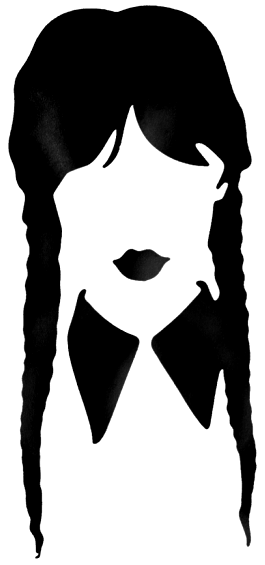
\includegraphics[height=1.35em]{figures/icons/mira-silhouette.png}}{}}}\enspace{\scshape\bfseries\color{black}Scene}\enspace\textperiodcentered\enspace{\bfseries #1}\pdblockheadingend{\itshape #2}}%
    \end{tcolorbox}\par\addvspace{8pt plus 2pt}%
  }%
  \long\def\xrefbox#1{\par\pd@settle\addvspace{4pt}\noindent\pd@marginhead{See also}{\small #1}\par\addvspace{4pt}}%
  % A generic "Thesis" margin label does not identify which claim matters.
  % Keep the prose; use an authored keyidea head only when it adds meaning.
  \long\def\pdthesis#1{\par\pd@settle\addvspace{6pt plus 1pt}\noindent#1\par\addvspace{6pt plus 1pt}}%
  \long\def\pullquote#1{\pdthesis{#1}}%
}
\makeatother

% Shared visual language for the seven analytical papers.
% This file defines marks, not layouts: every figure must still choose a grammar
% from its reader question.  The duplicate under whitepaper/figures is kept in
% lockstep for standalone Chapter I/II builds.
\usetikzlibrary{matrix,patterns.meta,shapes.geometric}

% ===========================================================================
% THE TYPOGRAPHIC LAW
% ===========================================================================
% Companion to the line-weight law in figures/pd-palette.tex (1px texture,
% 1.5px linework, 2px enclosure). Same shape of rule: name the roles, fix the
% values, one place.
%
% ONE SIZE. Every named text role in a figure is \pdfiglabelsize
% (= \footnotesize). Roles separate by WEIGHT, SLOPE, FAMILY and INK -- never
% by size. A fragment never writes a size command of its own; if a distinction
% needs making, it takes the role that makes it.
%
% Where the size comes from. Measured, not chosen:
%   \tiny  \scriptsize  \footnotesize  \small  \normalsize
%   5.23    6.97          8.72           9.55    10.46  pt   Book (10.5pt
%                                                            Pagella, 4.5in
%                                                            column, 7x10in)
%   5.98    7.97          8.97           9.96    10.91  pt   standalone chapter
%                                                            (11pt Latin Modern)
% \scriptsize renders at 6.97pt in the Book -- under figcheck's 7pt T1 floor
% before a single width promotion, so it is illegal by measurement, not taste.
% \footnotesize holds 8.72pt and still clears the floor at the 0.85 \resizebox
% limit craft-rules sets (7.41pt). It is also what the corpus already voted
% for: 78 of the 91 local font= declarations this law replaces were already
% \footnotesize, \footnotesize\bfseries or \footnotesize\itshape.
%
% \pdfigbasesize (= \small) is the tikzpicture's ambient size only, so an
% unstyled node is never SMALLER than a styled one; every named role steps
% down exactly one notch from it and none steps down twice.
%
% ONE FACE, AND IT IS THE DOCUMENT'S. \pdfiglabelfamily is empty by default,
% which means figure type inherits whatever face the document is setting --
% Palatino in the Book, Computer Modern in a standalone chapter. Figures
% agreeing with EACH OTHER is not the goal; figures agreeing with the
% paragraph beside them is. A fragment therefore never names a family. Not
% \sffamily (which resolves to Latin Modern Sans against a Computer Modern
% page and reads as a foreign object on it), not \rmfamily, not
% \fontfamily{...}. P18 in tikz_precheck.py is an error for exactly that.
% An edition MAY substitute a face -- the Swiss and technical editions set
% \pdfiglabelfamily to \pdgrotesk, because grotesk display is their declared
% character -- and it does so in ONE command in ONE file, so the substitution
% is a decision on the record rather than an accident in a fragment. The
% only family a fragment may ask for is the identifier one, and it asks for
% it by role (pd mono label / \pdfiglabelmono), never by \ttfamily.
%
% What the roles are, and what each one is for:
%   pd panel title        bold        the name of a panel
%   pd row label          bold        an actor/row name east of its lane
%   pd reverse row label  bold, cream a row name sitting on a dark band
%   pd axis label         regular     an axis title or a tick numeral
%   pd direct label       regular     a value or name riding its own mark
%   pd reverse label      regular, cream  a direct label on a dark band
%   pd mono label         mono        an identifier, path, or literal
%   pd verdict            bold        a terminal outcome stamp (CLEAR, REJECT)
%   pd note               italic      one aside per figure
%   pd legend             regular     a pgfplots legend entry
%   pd state / terminal / actor / artifact / decision   node text
%   pd axis               the whole pgfplots typographic block, one key
%   \pdfigsub             a gloss line under a heading INSIDE a node
%   \pdfigmath            math carrying a sub/superscript, inside a label
%
% A fragment that needs a compound style of its own composes it from a role
% above (`gate/.style={pd decision,minimum width=2cm}`), or, where no role
% fits, from the \pdfiglabel* handles here. It never writes a raw size
% command: P16 in skills/harbor-chartwork/scripts/tikz_precheck.py is an
% error for exactly that, and P10/P11 have been errors for \tiny and
% \scriptsize since before this law.
%
% What does NOT transfer from the screen rules these roles otherwise follow.
% The dataviz method those rules come from assumes an interactive chart: a
% tooltip carries any value a label could not fit, a filter row rescopes the
% view, hover lifts the hovered mark. A printed page has none of that, and the
% absence is not a defect to design around. The INTENT of the tooltip rule --
% "every value is reachable without gating" -- does transfer, and on this page
% it is discharged somewhere else: the value is in the caption, in the margin
% apparatus, or in the chapter's own worked example. So a label that will not
% fit inside its mark moves outside the mark or is dropped to the caption; it
% is never shrunk to fit, because there is no size below \footnotesize to shrink
% to, and never clipped. Do not add a hover affordance, a legend toggle, or a
% filter to a figure in this book.
%
% IDENTIFIERS GET ONE SPELLING. A key, a cell id, a file name or any other
% literal a reader could type is set in `pd mono label` (or \pdfiglabelmono
% inside a compound style), spelled exactly as the code spells it: sk_A, not
% skA and not sk with a subscript A; card0, not card-nought and not a Unicode
% subscript zero. A figure that shows the same identifier two ways has told
% the reader they are two things. The subscripted form belongs to MATHEMATICS
% ($\kappa_7$, an index into a sequence) and the literal form to CODE -- one
% figure may use both, for different objects, but never both for the same
% one. (A precheck for two spellings of one identifier inside a fragment is
% being added on another branch; this is the convention it will enforce.)
%
% SHAPE IS A CHANNEL, AND IT HAS TO SURVIVE THE PRINT SIZE. pd datum, pd
% focus datum and pd caution datum carry three different forms, because the
% house palette is three low-chroma print inks and every distinction it makes
% has to be doubled by something that is not colour. That only counts if the
% form is still legible at 2.1-2.7 pt: an edition that flattens all three to
% one form has removed the second channel and left the figure separating its
% classes by hue alone, which fails in greyscale and for a colour-blind
% reader. Any edition override that restyles a datum must keep three
% distinguishable forms, and must be checked on a render at 1.0x, not
% reasoned about from the point sizes.
%
% One screen rule that does NOT bind here, and why. "Text never wears the data
% colour" exists because a light categorical hue is illegible as text on a
% light surface. The house figure hues are print inks, not screen hues --
% hhink #1B1712, hhteal #00564C, hhamber #6B4500 -- and all three clear text
% contrast on cream, so a label MAY wear its series' ink to bind itself to a
% curve, which is direct labelling and saves a legend. The rule that survives
% is the reason behind it: text wears one of those three inks at full
% strength, or hhink!80!hhgray for recessive furniture, and nothing else. A
% tint of an ink (text=hhgray, text=hhteal!60) is not a role; it is a fade.
% ===========================================================================

\providecommand{\pdfiglabelfamily}{}            % an edition may set \pdgrotesk
\providecommand{\pdfiglabelsize}{\footnotesize} % every named text role
\providecommand{\pdfigbasesize}{\small}         % the picture's ambient size
\providecommand{\pdfiglabel}{\pdfiglabelfamily\pdfiglabelsize}
\providecommand{\pdfiglabelbold}{\pdfiglabel\bfseries}
\providecommand{\pdfiglabelitalic}{\pdfiglabel\itshape}
\providecommand{\pdfiglabelmono}{\pdfiglabelsize\ttfamily}
% The one role that is not a node style, because it lives INSIDE a node's text:
% the second line under a heading that glosses it ("reviewer role / obligation +
% capability + authority"). Every fragment that needed it reached for \tiny or
% \scriptsize, which is how seven \tiny and twelve \scriptsize survived P10/P11
% as hard errors in the corpus. It steps down by SLOPE and WEIGHT, not size, so
% it stays legible and stays legal, and it touches neither family nor ink --
% which is what lets it sit on a reversed node without vanishing.
\providecommand{\pdfigsub}{\mdseries\itshape}
% The one place the law's own size is not the right size, with the measurement
% that says so. A subscript is set at roughly 70% of its base, so math with a
% subscript inside a \pdfiglabelsize label renders its subscript at 5.98pt in a
% standalone chapter and 6.36pt in the Book -- under figcheck's 7pt T1 floor,
% measured, not estimated. One notch up puts the same subscript at 7.97pt and
% 7.64pt, over the floor, while the base glyph stays close enough to its
% neighbours that the label still reads as one label. Use it ONLY for a math
% group that carries a sub- or superscript; plain math takes the label's own
% size like any other text.
\providecommand{\pdfigmath}{\normalsize}

% ---------------------------------------------------------------------------
% THE GUIDE DASH, IN ABSOLUTE POINTS, IN ONE PLACE.
%
% `pd guide` used to read `line width=.45pt,densely dotted`. `densely dotted`
% expands to `dash pattern=on \pgflinewidth off 1pt`, and \pgflinewidth is read
% when the KEY is processed, not when the path is stroked. So the Swiss
% edition's `pd guide/.append style={draw=hhink!40,line width=.5pt}` widened the
% stroke and left the dash at the .45pt already baked into it. The canonical
% Book therefore shipped a 0.448pt dot on a 0.498pt stroke.
%
% Measured on the Book (Swiss, the built edition) at 1.0x / 150 dpi:
%   on 0.448pt = 0.93 device px -- UNDER ONE PIXEL
%   off 0.996pt = 2.08 px, period 3.01 px
%   peak ink per dot swings 0.173-0.345 (a 2.0x range) purely with where the
%     dot lands on the pixel grid; the line's weight is a rasteriser accident
%   the darkest pixel of the guide (0.30) is DARKER than every pixel of the
%     solid `pd hairline` (0.25/0.19) beside it, while its mean ink (2.3%) is a
%     quarter of the hairline's (8.9%) -- the two lines are not separated on any
%     axis a reader can name
%   declared separation from `pd hairline`: hhink!40 against hhink!45, 4.6% of
%     the grey scale
%
% So a fragment that used `pd guide` to mean "this line is not that line" was
% relying on ink that does not arrive on the page. Twenty-five of the corpus's
% thirty-six guide draws carry exactly that meaning.
%
% The replacement is stated absolutely and measures phase-STABLE: every dot
% renders at the same weight wherever it falls on the grid (peak column ink
% 0.808, invariant across twelve sub-pixel offsets). It is a macro rather than
% three numbers because an edition that restates one of them and not the others
% is how this defect happened. The geometry is a LEGIBILITY FLOOR, not an
% edition's character: an edition may move the guide's ink, and states the
% geometry through these two macros so it cannot half-restate it.
%
% Any dash in this corpus is stated in absolute points. The `dotted` family
% (`dotted`, `densely dotted`, `loosely dotted`) derives its on-length from the
% line width and is therefore banned -- P23 in tikz_precheck.py. `dashed` and
% its relatives are absolute (on 3pt off 3pt) and are fine.
\providecommand{\pdguidewidth}{.7pt}
% Three lengths, not one macro holding the whole key: pgfkeys splits a key list
% on `,` and `=` before expanding anything (so a macro carrying `dash
% pattern=...` is read as one key NAME), and TikZ's dash-pattern scanner reads
% the literal words `on`/`off` without expanding a macro that hides them. A
% dimension after each word does expand, which is the seam that works.
\providecommand{\pdguideon}{1.2pt}
\providecommand{\pdguideoff}{2.0pt}

\tikzset{
  pd figure/.style={font=\pdfiglabelfamily\pdfigbasesize,text=hhink},
  pd hairline/.style={draw=hhgray!78,line width=.5pt},
  pd rule/.style={draw=hhink,line width=.62pt},
  pd focus rule/.style={draw=hhteal,line width=1.05pt},
  pd caution rule/.style={draw=hhamber,line width=1.05pt},
  % Darker per dot than the hairline, lighter in mean ink than it: a guide is a
  % construction line the reader traces from a mark to an axis, so each dot has
  % to be a definite mark, while the line as a whole has to recede behind the
  % data. The hairline is the opposite -- continuous and faint. Those are the
  % two axes that now separate them, instead of 4.6% of the grey scale.
  pd guide/.style={draw=hhink!70,line width=\pdguidewidth,dash pattern=on \pdguideon off \pdguideoff},
  % A LATTICE is the rule work a figure stands on: column separators, row
  % baselines, a time grid. It is NOT dotted, and that is the point. Dotted
  % versus solid is a semantic channel -- it distinguishes a construction line
  % from a drawn edge -- and thirteen fragments were spending it on background
  % grid where it distinguishes nothing. A dash that carries no meaning is the
  % first ink a rasteriser is entitled to lose, and it did. A lattice is
  % continuous and quiet; a guide is discontinuous and definite. Use `pd guide`
  % only where the reader must see that the line is not a drawn edge.
  pd lattice/.style={draw=hhgray!52,line width=.4pt},
  pd arrow/.style={-{Stealth[length=2.0mm,width=1.25mm]},draw=hhink,line width=.68pt},
  pd focus arrow/.style={-{Stealth[length=2.0mm,width=1.25mm]},draw=hhteal,line width=.88pt},
  pd caution arrow/.style={-{Stealth[length=2.0mm,width=1.25mm]},draw=hhamber,line width=.88pt,dashed},
  pd row label/.style={font=\pdfiglabelbold,text=hhink,anchor=east},
  pd panel title/.style={font=\pdfiglabelbold,text=hhink,align=left},
  pd axis label/.style={font=\pdfiglabel,text=hhink!80!hhgray},
  % inner ysep is deliberately larger than inner xsep: at 1.5pt the descenders
  % of a last line (q, y, p, g) reach the bottom of the cream backing under
  % Computer Modern, where they clear it under Palatino. A label should not
  % need its own patch to hold its own tails, and the sensitivity is the
  % face's, not the fragment's.
  pd direct label/.style={font=\pdfiglabel,text=hhink,align=left,
    inner xsep=1.5pt,inner ysep=2.5pt,fill=hhpaper},
  pd note/.style={font=\pdfiglabelitalic,text=hhink!80!hhgray,align=left},
  pd tick/.style={draw=hhgray,line width=.45pt},
  pd datum/.style={circle,fill=hhink,draw=none,inner sep=2.1pt},
  pd focus datum/.style={circle,fill=hhteal,draw=hhpaper,line width=.55pt,inner sep=2.5pt},
  pd caution datum/.style={diamond,fill=hhamber,draw=hhpaper,line width=.55pt,inner sep=2.5pt},
  pd state/.style={draw=hhink,line width=.62pt,fill=hhsand!30,rounded corners=1.5pt,
    font=\pdfiglabel,inner xsep=8pt,inner ysep=6pt,align=center,minimum height=9mm},
  pd terminal/.style={pd state,double,double distance=1.2pt},
  pd actor/.style={draw=hhink,line width=.62pt,fill=hhpaper,rounded corners=1.5pt,
    font=\pdfiglabel,inner xsep=8pt,inner ysep=5pt,align=center},
  pd artifact/.style={draw=hhgray!80,line width=.55pt,fill=hhsand!30,
    font=\pdfiglabel,inner xsep=8pt,inner ysep=5pt,align=center},
  pd boundary/.style={draw=hhgray!70,line width=.55pt,dashed,rounded corners=2pt},
  % These three are pale washes: they are frequently layered on top of `pd
  % state` (directly, or via a compound style like `cell`), whose swiss-edition
  % override (figures/pd-figure-language-swiss.tex) appends text=hhpaper for the
  % common case of a solid, saturated fill. A pale wash is the opposite case --
  % text must stay dark ink regardless of what came before it in the style
  % list, so each one restates text=hhink explicitly rather than relying on
  % whatever was inherited.
  pd focus fill/.style={fill=hhteal!24,draw=hhteal!65,line width=.4pt,text=hhink},
  pd caution fill/.style={fill=hhamber!26,draw=hhamber!70,line width=.4pt,text=hhink},
  pd neutral fill/.style={fill=hhsand!40,draw=hhgray!65,line width=.4pt,text=hhink},
  pd ink fill/.style={fill=hhink,draw=hhink,line width=.4pt,text=hhpaper},
  pd hatch/.style={pattern={Lines[angle=45,distance=4pt,line width=.28pt]},pattern color=hhgray!55},
  % --- roles the corpus was inventing locally, now named -------------------
  % Each is built ON TOP of the role it varies, so an edition's .append style
  % on the parent reaches it without the edition file having to list it.
  pd decision/.style={pd state,diamond,aspect=1.55,font=\pdfiglabelbold,
    minimum height=0pt,inner xsep=3pt,inner ysep=3pt},
  % A shade more side bearing than its parent: a monospace glyph box overhangs
  % its own advance width, so the cream backing at the parent's 1.5pt clipped
  % the last character of a long identifier.
  pd mono label/.style={pd direct label,font=\pdfiglabelmono,inner xsep=2.5pt,inner ysep=2.5pt},
  pd verdict/.style={pd direct label,font=\pdfiglabelbold},
  pd reverse label/.style={pd direct label,text=hhpaper,fill=none},
  pd reverse row label/.style={pd row label,text=hhpaper},
  pd legend/.style={font=\pdfiglabel,text=hhink,draw=none,fill=none},
  % A KIND TAG names what a row or column IS, rather than what it says: an
  % audience ("for the operator"), a category, a running head. craft-rules S6
  % already reserves small caps for exactly this, and small caps is the
  % smallest effective difference that marks a change in kind -- it needs no
  % size drop, no second colour and no box.
  pd kind tag/.style={pd axis label,font=\pdfiglabel\scshape,align=right},
  % A BADGE is a short boxed fact riding beside a row -- a part and chapter
  % range, a version, a count. Hairline edge, no fill: it is a label with a
  % boundary, not a region.
  pd badge/.style={pd hairline,font=\pdfiglabel,text=hhink,align=center,
    inner sep=2.4pt,fill=none},
}

% The pgfplots half of the same law. Before this existed, every plot fragment
% restated title style/label style/tick label style by hand, and they disagreed
% -- four said the tick numerals were hhink!80!hhgray, three said hhgray, and
% the axis rule was drawn four different ways. `pd axis` is the one place now.
% The axis line is `pd hairline` because an axis is reference furniture, not
% data: heavy for data, light for the frame that carries it.
\ifdefined\pgfplotsset
\pgfplotsset{
  pd axis/.style={
    title style={font=\pdfiglabelbold,text=hhink,yshift=-2pt},
    label style={font=\pdfiglabel,text=hhink!80!hhgray},
    tick label style={font=\pdfiglabel,text=hhink!80!hhgray},
    legend style={pd legend},
    axis line style={pd hairline},
    tick style={pd tick},
  },
}
\fi

% Small reusable marks.  They deliberately avoid prose-bearing boxes.
\newcommand{\pdfigaxis}[4]{%
  \draw[pd rule,-{Stealth[length=1.65mm,width=1.05mm]}] (#1,#2) -- (#3,#2);
  \node[pd axis label,anchor=west] at (#3,#2) {#4};
}
\newcommand{\pdfigvaxis}[4]{%
  \draw[pd rule,-{Stealth[length=1.65mm,width=1.05mm]}] (#1,#2) -- (#1,#3);
  \node[pd axis label,anchor=south,align=center] at (#1,#3) {#4};
}

% ---------------------------------------------------------------------------
% Editions. The Book sets \pdedition (maritime | swiss | technical) and the
% matching override file restyles the same names, so one drawing renders in
% each edition's character. Standalone chapters have no edition. An edition
% changes the FAMILY (via \pdfiglabelfamily) and the character of the marks;
% it never changes the size, because the size is the law above.
% ---------------------------------------------------------------------------
\ifdefined\pdedition\IfFileExists{figures/pd-figure-language-\pdedition.tex}{\input{figures/pd-figure-language-\pdedition}}{}\fi


\providecommand{\keyidea}[1]{}
\providecommand{\pitfall}[1]{}
\providecommand{\scene}[2]{}
\providecommand{\xrefbox}[1]{}
\providecommand{\pullquote}[1]{}
\providecommand{\pdchapref}[2]{\textbf{#2}}
\providecommand{\pdmarginfigure}[2]{}
\providecommand{\Cref}[1]{\ref{#1}}
\providecommand{\cref}[1]{\ref{#1}}

\title{\textbf{Chapter 0: Foundations and Prerequisites}\\
\large Pre-LLM Multi-Agent Theory, Transformer Mechanics, and the Kernel Gap}
\author{The Authors}
\date{September 2026}

\begin{document}

\maketitle


\noindent\emph{Express lane: Before constructing an operating kernel for autonomous systems, we must establish the physical and theoretical ground upon which modern AI agents stand. This chapter establishes eight core foundations assumed by the subsequent eight chapters: (i)~the dual lineage of autonomous agency connecting classical symbolic multi-agent systems to generative connectionism; (ii)~classical multi-agent theory, spanning Bratman practical rationality, Rao--Georgeff $BDI_{CTL^*}$ temporal logic, AgentSpeak(L) operational semantics, normative deontic reasoning, Hewitt--Agha actor concurrency versus Hoare CSP, FIPA-00037 speech acts, Smith's Contract Net Protocol, Big Brother dynamic epistemic logic, and game-theoretic mechanism design; (iii)~modern coding agent architectures, contrasting leading systems and formalizing closed-loop POMDP deliberation (ReAct, Tree of Thoughts, Reflexion); (iv)~cognitive control, tool-call SFT, PRMs, and test-time compute; (v)~transformer mechanics, KV-cache memory scaling, and context economics; (vi)~the tool execution hypervisor, MCP protocols, skill progressive disclosure, and Ramadge--Wonham supervisory control hooks; (vii)~multi-agent swarm topologies, durable identity versus ephemeral leases, and zombie salvage; and (viii)~the kernel gap, proving mathematically why generative models cannot act as their own operating system.}

\section{Introduction: The Unit of Account and the Dual Lineage}

\pdmarginfigure{hobbes}{Thomas Hobbes framed the sovereign Commonwealth as an artificial man; autonomous software requires the same institutional structure to prevent destructive races.}%
Agentic software is usually measured by the agent: capability, runtime, tool
access, and parallel copies. That is the wrong unit of account. A process may
disappear, rename itself, summarize its mistakes, or hand work off. The durable
object must be the work: its authorization, permitted effects, evidence, open
obligations, and liability for the outcome.

\subsection{The Dual Lineage of Autonomous Agency}

Autonomous software agents did not begin with large language models. The problem of coordinating multiple independent computational processes, each pursuing distinct local goals under incomplete information and bounded resources, has occupied distributed systems and artificial intelligence research for over four decades.

When a modern coding agent inspects a git repository, evaluates compiler diagnostics, plans a refactoring sequence, and invokes a bash shell, it operates at the intersection of two previously separate research lineages:
\begin{enumerate}[leftmargin=1.8em,itemsep=2pt]
  \item \textbf{Symbolic Multi-Agent Systems (1975--2010):} Mathematical formalisms for practical rationality, intention persistence, asynchronous message passing, contract negotiation, epistemic logic, and social norms.
  \item \textbf{Statistical Connectionism (2017--2026):} Deep autoregressive sequence prediction trained over planet-scale code and natural language corpora, capable of zero-shot semantic reasoning, code synthesis, and tool parameterization.
\end{enumerate}

The tension between these lineages defines the subject of this textbook. Modern frontier models supply unprecedented semantic reasoning, but possess neither persistent state, monotonic capability boundaries, nor physical execution guarantees. When an ungrounded model encounters an unexpected tool error, its probabilistic nature induces intention drift, hallucinatory claims of success, and concurrency hazards. To scale from an isolated interactive coding assistant to a collaborative, multi-agent autonomous engineering fleet, we must place statistical inference inside an authoritative, mathematically verified structural envelope where the unit of account is the work rather than the ephemeral process.

\subsection{Eight Propositions of Accountable Coordination}

This book develops that claim in eight propositions, one per chapter, in the
order the book is read:

\begin{enumerate}[leftmargin=2.1em,itemsep=2pt,topsep=4pt]
  \item \textbf{Prevention begins at the effect boundary (\pdchapref{swk}{The Single-Writer Kernel}).} Rules can be enforced
  before an act only when the system controls the channel through which the act
  occurs. Local effects therefore pass through one serial authority; semantic
  failures that no gate can decide remain matters of detection and remedy.

  \item \textbf{Delegation only narrows (\pdchapref{anchor}{The Anchor Protocol}).} Every child capability is a strict
  subset of its parent's authority and lifetime. Authentication says who signed;
  attenuation says what the signature may authorize. Both are needed at every
  hop.

  \item \textbf{Confinement is a property of the room, not of the tenant (\pdchapref{sealed}{The Sealed Harbor}).}
  Two owners who trust neither each other nor the venue can still take one
  answer out of a sealed room when its only exit is a metered slot: silence
  except through the slot, a gate on the only enforceable boundary, a budget
  that conserves, and canaries for what the gate cannot prove. What the room
  cannot promise is stated as a limit, at the same prominence as the claims.

  \item \textbf{Supervision has an information cost (\pdchapref{ls}{Attention and Supervision}).} \pdmarginfigure{shannon}{Claude Shannon derived the mathematical bounds on information transmission; human supervision cannot compress fleet telemetry below its entropy rate.}%
  A digest cannot guarantee
  that a human will notice any one of many relevant events unless it spends
  enough bits, attention, or artifact openings to distinguish them. A summary
  is therefore an index into evidence, not a substitute for it.

  \item \textbf{Accountability must outlive the process (\pdchapref{spawn}{Spawn-to-Person}).} A task acquires a
  durable principal, capability history, evidence record, obligations, and
  outcome. Restarting an agent or choosing a new name must not erase that case
  file or refill the resources it already consumed.

  \item \textbf{Exchange requires separated instruments (\pdchapref{tx}{Agent Transactions}).} Payment rewards the
  requested work. Collateral prices a bounded failure. Evidence supports a
  claim. Settlement closes it exactly once. Combining those functions in one
  score or token makes each of them less trustworthy.

  \item \textbf{Uncertainty needs an institution (\pdchapref{econ}{The Harbor Economy}).} Some harms cannot be
  prevented and some outcomes cannot be judged mechanically. Witnesses,
  randomized audits, bounded bonds, appeals, and conservation rules turn that
  residual uncertainty into a process that can be inspected and contested.

  \item \textbf{Federation relays evidence, not sovereignty (\pdchapref{fed}{Federated Harbors}).} Mutually
  distrustful machines may exchange signed capabilities, revocations, witness
  roots, and settlement claims without sharing a database or accepting a global
  ruler. Transport can carry evidence; it cannot decide what either machine is
  permitted to do with it.
\end{enumerate}

Read these as a dependency chain: each chapter uses earlier mechanisms and
states what they cannot guarantee.

\subsection{What Counts as Knowing: Epistemic Bounds and Evidence Channels}
\pdmarginfigure{lovelace}{Ada Lovelace observed that analytical engines have no pretensions to originate anything; they execute what we know how to order them to perform.}%
Every consequential statement in this volume has a status and a boundary. Derivations establish
relations under named assumptions. Finite checks exhaust a stated state space,
not every deployment. Simulations estimate behavior under a stated generator;
repository tests exercise named paths; running code proves availability, not
universal mediation. Counterexamples remain in the record because they mark
claims the research killed rather than conclusions it merely failed to prove.

Evidence is typed as well. When a chapter reports what a harbor observed, it
names the channel that produced the observation, and each channel has a blind
spot that no amount of volume removes:
\begin{itemize}[leftmargin=1.8em,itemsep=2pt]
  \item A \emph{deterministic verifier} (a test, a type checker, a model checker) shows that a stated property holds of the artifact it examined, and nothing about properties it did not state.
  \item A \emph{provenance witness} (a signature, a hash, a Merkle inclusion, an append-only log) shows attribution and tamper-evidence relative to a commitment, never that every event was logged or that a description is true.
  \item A \emph{protected meter} (a counter its subject cannot rewrite) shows a quantity, not its cause.
  \item \emph{Expert judgment} shows an assessment under a named rubric and carries the assessor's error rate.
  \item \emph{Buyer preference} shows what was chosen, not that the choice was right.
  \item A \emph{delayed outcome} shows what happened, and arrives too late to prevent it.
\end{itemize}
The reader should ask the same question of any dashboard: which channel, and what can it not show.

\Cref{app:volume-status} gives the implementation boundary;
\cref{app:result-atlas} records the results and their limits. The companion
\path{docs/harbor-research/mega-volume-epistemic-manifest.yaml} preserves each
result's source, status, conditions, boundary, chapter home, and verification
artifact. The chapters stand alone; the book's claim is the chain they make.

\section{Classical Multi-Agent Systems Foundations}

Before analyzing neural coding agents, we formalize the foundational frameworks developed during the classical era of multi-agent systems.

\subsection{Intentional Agency and Practical Rationality}

Classical decision theory models an agent as an expected utility maximizer balancing subjective beliefs $\mathcal{B}$ and desires $\mathcal{D}$. In his seminal 1987 work \emph{Intention, Plans, and Practical Reason}, philosopher Michael Bratman demonstrated that this two-component model is computationally inadequate for resource-bounded agents operating in dynamic environments~\cite{bratman1987intention}.

A resource-bounded agent cannot continuously compute optimal policies from first principles at every millisecond. Practical rationality requires a third mental attitude: \textbf{Intention} ($\mathcal{I}$). Intentions are not merely desires with high utility; they represent \emph{conduct-controlling pro-attitudes to which the agent has actively committed}.

Bratman established four defining functional roles of intentions:
\begin{enumerate}[leftmargin=1.8em,itemsep=2pt]
  \item \textbf{Drive Means-End Reasoning:} An intention to achieve goal $\phi$ obligates the agent to formulate sub-plans and allocate computational cycles until $\phi$ is satisfied.
  \item \textbf{Filter of Admissibility:} Once an intention $\phi$ is adopted, candidate options inconsistent with $\phi$ (given current beliefs $\mathcal{B}$) are ruled inadmissible without evaluating their cost-benefit payoff.
  \item \textbf{Stability and Commitment:} Intentions resist reconsideration in the absence of relevant environmental interrupts or belief updates, preventing computational paralysis.
  \item \textbf{Coordination Scaffolding:} Intentions enable interpersonal coordination: other agents can safely form expectations regarding an agent's future actions based on its declared commitments.
\end{enumerate}

\subsection{The Rao--Georgeff BDI Temporal Logic (\texorpdfstring{$BDI_{CTL^*}$}{BDI-CTL*})}

Rao and Georgeff~\cite{rao1991modeling,rao1995bdi} formalized Bratman's theory into a multimodal branching-time temporal logic ($BDI_{CTL^*}$). A temporal world model $\mathcal{M}$ is defined as an 8-tuple:
\begin{equation}
\mathcal{M} \;=\; \langle W, T, \prec, U, \mathcal{B}, \mathcal{D}, \mathcal{I}, \Phi \rangle
\end{equation}
where $W$ is a set of possible worlds, $T$ is a discrete set of time points ordered by tree-branching relation $\prec$, $U$ is the universe of discourse, $\Phi$ interprets predicates across worlds and times, and $\mathcal{B}, \mathcal{D}, \mathcal{I} \subseteq W \times T \times W$ are accessibility relations for Beliefs, Desires, and Intentions.

For world $w \in W$ at time $t \in T$:
\begin{align}
\mathcal{B}_t(w) &= \{ w' \in W \mid (w, t, w') \in \mathcal{B} \} \\
\mathcal{D}_t(w) &= \{ w' \in W \mid (w, t, w') \in \mathcal{D} \} \\
\mathcal{I}_t(w) &= \{ w' \in W \mid (w, t, w') \in \mathcal{I} \}
\end{align}

Semantics of the mental modalities at state $\langle w, t \rangle$:
\begin{align}
\mathcal{M}, w, t \models \mathrm{Bel}(\phi) &\iff \forall w' \in \mathcal{B}_t(w), \; \mathcal{M}, w', t \models \phi \\
\mathcal{M}, w, t \models \mathrm{Des}(\phi) &\iff \forall w' \in \mathcal{D}_t(w), \; \mathcal{M}, w', t \models \phi \\
\mathcal{M}, w, t \models \mathrm{Int}(\phi) &\iff \forall w' \in \mathcal{I}_t(w), \; \mathcal{M}, w', t \models \phi
\end{align}

Beliefs satisfy the $KD45$ axiom system (deductive closure $\mathbf{K}$, consistency $\mathbf{D}$, positive introspection $\mathbf{4}$, and negative introspection $\mathbf{5}$). Desires and Intentions satisfy seriality ($\mathbf{D}$), ensuring an agent never desires or intends logical contradictions ($\neg\mathrm{Des}(\bot)$ and $\neg\mathrm{Int}(\bot)$).

\subsubsection{Compatibility and Weak Realism}
In rational agency, an agent's desires and intentions must be constrained by its beliefs. Under the \textbf{Weak Realism} axiom, an agent cannot intend what it believes to be impossible:
\begin{equation}
\forall w \in W, \; \mathcal{I}_t(w) \cap \mathcal{B}_t(w) \neq \emptyset
\end{equation}
Syntactically, for temporal achievement goals:
\begin{equation}
\mathrm{Int}(\mathbf{A}\lozenge \phi) \;\to\; \neg\mathrm{Bel}(\neg\mathbf{E}\lozenge \phi)
\end{equation}
where $\mathbf{A}\lozenge \phi$ denotes ``$\phi$ holds eventually on all future paths,'' and $\mathbf{E}\lozenge \phi$ denotes ``$\phi$ holds on at least one branch.''

\subsection{Formal Commitment Strategies}

A commitment strategy dictates the precise formal conditions under which an agent drops an intention $\phi$. Rao and Georgeff~\cite{rao1991modeling} formalized three canonical strategies:

\begin{table}[H]
\centering
\small
\begin{tabularx}{\textwidth}{lX}
\toprule
\textbf{Commitment Strategy} & \textbf{Formal Drop Axiom} \\
\midrule
\textbf{Blind (Fanatical)} & Maintains $\mathrm{Int}(\mathbf{A}\lozenge \phi)$ until $\mathrm{Bel}(\phi)$ holds. \\
& $\mathrm{Int}(\mathbf{A}\lozenge \phi) \land \neg\mathrm{Bel}(\phi) \to \mathbf{A}\big(\mathrm{Int}(\mathbf{A}\lozenge \phi) \;\mathcal{U}\; \mathrm{Bel}(\phi)\big)$. \\
& \emph{Pathology:} Induces infinite loops if $\phi$ becomes physically impossible. \\
\addlinespace[3pt]
\textbf{Single-Minded} & Drops $\phi$ if achieved \emph{or} believed impossible. \\
& $\mathrm{Int}(\mathbf{A}\lozenge \phi) \land \neg\mathrm{Bel}(\phi) \land \mathrm{Bel}(\mathbf{E}\lozenge \phi) \to \mathbf{A}\big(\mathrm{Int}(\mathbf{A}\lozenge \phi) \;\mathcal{U}\; (\mathrm{Bel}(\phi) \lor \neg\mathrm{Bel}(\mathbf{E}\lozenge \phi))\big)$. \\
& \emph{Standard:} Balances persistence with dynamic feasibility. \\
\addlinespace[3pt]
\textbf{Open-Minded} & Drops $\phi$ if achieved, impossible, \emph{or no longer desired}. \\
& $\mathrm{Int}(\mathbf{A}\lozenge \phi) \land \dots \land \mathrm{Des}(\mathbf{A}\lozenge \phi) \to \mathbf{A}\big(\mathrm{Int}(\mathbf{A}\lozenge \phi) \;\mathcal{U}\; (\mathrm{Bel}(\phi) \lor \neg\mathrm{Bel}(\mathbf{E}\lozenge \phi) \lor \neg\mathrm{Des}(\mathbf{A}\lozenge \phi))\big)$. \\
\bottomrule
\end{tabularx}
\caption{Canonical commitment strategies in BDI agent architectures.}
\label{tab:commitment-strategies}
\end{table}

\begin{pdclaim}{Design invariant}{Commitment Persistence}\label{inv:commitment-persistence}
An agent's intention $\iota \in \mathcal{I}$ must not be abandoned merely because a single step incurs a transient tool failure. Intention reconsideration is an explicit state transition triggered by invariant failure or objective discharge, not an accidental consequence of context window truncation.
\end{pdclaim}

\subsection{Operational Semantics of AgentSpeak(L) and Normative Extensions}

AgentSpeak(L)~\cite{bordini2007agentspeak} provides structural operational semantics (SOS) for executing BDI agents. An agent configuration is a tuple $C = \langle bs, ps, is, \mathcal{E}, A \rangle$, where $bs$ is the belief base, $ps$ is the plan library, $is$ is the set of active intention stacks, $\mathcal{E}$ is the event queue, and $A$ is the action history.

The operational execution cycle is governed by three deterministic or priority-driven selection functions:
\begin{enumerate}[leftmargin=1.8em,itemsep=2pt]
  \item $S_E(\mathcal{E}) = \langle te, i \rangle$: Selects an event from $\mathcal{E}$ (e.g., belief change $+b$, goal addition $+!g$).
  \item $S_O(\mathrm{App})$: Selects a plan $(p, \theta)$ from the applicable plans whose context is entailed by $bs\theta$.
  \item $S_I(is) = i$: Selects which intention stack advances its execution step in the current cycle.
\end{enumerate}

When an action $a$ in plan $p$ fails during host execution, AgentSpeak semantics do not silently abort the agent; instead, the failure transition posts a failure event $-!g$ to $\mathcal{E}$, popping the failed plan frame and invoking explicit recovery plans:
\begin{equation}
\frac{\epsilon = \langle te, i \rangle, \quad \mathrm{App}(\mathrm{Rel}(te, ps), bs) = \emptyset}{\langle bs, ps, is, \mathcal{E}, A \rangle \;\longrightarrow\; \langle bs, ps, is, \mathcal{E} \cup \{\langle -!g, \mathrm{pop}(i) \rangle\}, A \rangle}
\end{equation}

\subsubsection{Normative Extensions: Deontic Constraints and Regret Minimization}
In institutional multi-agent systems, agents are constrained by external \textbf{norms} (deontic logic). A norm is defined as a 6-tuple $N = \langle \text{id}, \text{Type}, \phi_{\text{act}}, \phi_{\text{tgt}}, d, \text{Sanction} \rangle$, where $\text{Type} \in \{\mathcal{O}, \mathcal{F}, \mathcal{P}\}$ (Obligation, Prohibition, Permission), $\phi_{\text{act}}$ is the activation context, $\phi_{\text{tgt}}$ is the target state, $d$ is the deadline, and $\text{Sanction}$ is the penalty for violation.

To reconcile institutional norms with internal intentions, agents maintain an \textbf{Abstract Norm Base} ($ANB$) and evaluate instantiated norms in the \textbf{Norm Instance Base} ($NIB$). When norm instances conflict with active goals ($Plans(is \cup \mathcal{N}) = \emptyset$), the agent resolves the normative conflict by partitioning candidate norms into \textbf{Maximal Non-Conflicting Subsets} (MNCS), selecting the subset that minimizes maximum penalty under a \textbf{minimax regret} criterion:
\begin{equation}
S^* \;=\; \arg\min_{S \in \Omega} \;\max_{n_v \in \mathcal{N} \setminus S} \;\mathrm{Cost}(\mathrm{Sanction}(n_v))
\end{equation}
This ensures that any deliberate norm violation is recorded in an immutable ledger alongside its formal justification.

\subsection{Concurrency: Hewitt--Agha Actor Model vs. Hoare CSP}

Multi-agent coordination requires formal concurrency models. Classical computer science produced two foundational, mathematically rigorous paradigms for message-passing concurrency:

\begin{table}[H]
\centering
\small
\begin{tabularx}{\textwidth}{lXX}
\toprule
\textbf{Dimension} & \textbf{Hewitt--Agha Actor Model~\cite{hewitt1973actor,agha1986actors}} & \textbf{Hoare's CSP (1978)~\cite{hoare1978csp}} \\
\midrule
\textbf{Primitive} & Autonomous Actor with private state & Sequential Process and Named Channel \\
\textbf{Synchronization} & Asynchronous (non-blocking send) & Synchronous (rendezvous handshake) \\
\textbf{Addressing} & First-class Mailbox addresses & Explicit Channel identifiers \\
\textbf{Buffering} & Unbounded mailbox queue & Zero buffer (unbuffered channels) \\
\textbf{State Evolution} & Replacement behavior ($\mathtt{become}(B')$) & Sequential instruction trace \\
\textbf{Failure Mode} & Mailbox overflow; unhandled messages & Circular rendezvous deadlock \\
\textbf{Modern Descendant} & Erlang/OTP, Akka, Ray, agentsd & Go channels, Rust crossbeam \\
\bottomrule
\end{tabularx}
\caption{Message-passing concurrency: Hewitt--Agha actors versus Hoare CSP.}
\label{tab:concurrency-models}
\end{table}

In the Actor model, an actor processes one message from its mailbox by executing a bounded 3-tuple:
\begin{equation}
\mathrm{Actor}(S, m) \;\xrightarrow{\text{atomic}}\; \big( S',\; \{m_1, \dots, m_k\},\; \{\alpha_{\mathrm{new},1}, \dots, \alpha_{\mathrm{new},j}\} \big)
\end{equation}
where $S'$ is the designated replacement behavior, $\{m_k\}$ are asynchronous outbound messages, and $\{\alpha_{\mathrm{new}}\}$ are newly spawned actors. This share-nothing encapsulation provides the blueprint for sandboxed agent processes.

\clearpage
\subsection{Communicative Action and Speech Acts (FIPA-00037)}

Standard computer networks exchange raw data packets; autonomous agents exchange \textbf{speech acts}. Grounded in Austin's distinction between locutionary (syntactic utterance), illocutionary (communicative intent), and perlocutionary (consequential effect) acts~\cite{austin1962how}, and Searle's taxonomy of illocutionary forces~\cite{searle1969speech}, the Foundation for Intelligent Physical Agents standardized the \textbf{FIPA ACL Communicative Act Library} (FIPA-00037)~\cite{fipa2002acl}.

Every communicative act $a(s, r, \phi)$ between sender $s$ and receiver $r$ is formally defined by its \textbf{Feasibility Preconditions} ($FP$) and intended \textbf{Rational Effect} ($RE$):

\begin{table}[H]
\centering
\footnotesize
\setlength{\tabcolsep}{3pt}
\begin{tabularx}{\textwidth}{l l >{\raggedright\arraybackslash}X >{\raggedright\arraybackslash}X}
\toprule
\textbf{Act} & \textbf{Category} & \textbf{Feasibility Precondition ($FP$)} & \textbf{Rational Effect ($RE$)} \\
\midrule
\texttt{inform} & Assertive & $\mathrm{Bel}_s(\phi) \land \neg\mathrm{Bel}_s(\mathrm{Bel}_r(\phi))$ & $\mathrm{Bel}_r(\phi)$ \\
\texttt{request} & Directive & $\mathrm{FP}(\alpha)[s\backslash r] \land \mathrm{Bel}_s(\mathrm{Agent}(r, \alpha))$ & $\mathrm{Done}(\alpha)$ \\
\texttt{query-if} & Directive & $\neg\mathrm{Bel}_s(\phi) \land \neg\mathrm{Bel}_s(\neg\phi)$ & $\mathrm{Bel}_s(\mathrm{Bel}_r(\phi) \lor \mathrm{Bel}_r(\neg\phi))$ \\
\texttt{propose} & Commissive & $\mathrm{Bel}_s(\mathrm{Int}_s(\mathrm{Done}(\alpha, \phi)))$ & $\mathrm{Bel}_r(\mathrm{Int}_s(\mathrm{Done}(\alpha, \phi)))$ \\
\texttt{agree} & Commissive & $\mathrm{Bel}_s(\mathrm{Int}_s(\mathrm{Done}(\alpha)))$ & $\mathrm{Bel}_r(\mathrm{Int}_s(\mathrm{Done}(\alpha)))$ \\
\texttt{refuse} & Directive & $\mathrm{Bel}_s(\neg\mathrm{Int}_s(\mathrm{Done}(\alpha)))$ & $\mathrm{Bel}_r(\neg\mathrm{Int}_s(\mathrm{Done}(\alpha)))$ \\
\texttt{failure} & Assertive & $\mathrm{Bel}_s(\mathrm{Failed}(\alpha, \psi))$ & $\mathrm{Bel}_r(\mathrm{Failed}(\alpha, \psi))$ \\
\bottomrule
\end{tabularx}
\caption{FIPA-00037 communicative performatives with mental-state preconditions and rational effects.}
\label{tab:fipa-performatives}
\end{table}

In an autonomous agent operating kernel, performatives cease to be informal text; they are cryptographically signed, immutable protocol events backed by content-addressed receipts.

\subsection{Task Allocation: Smith's Contract Net Protocol (1980)}

Reid G. Smith's (1980) \textbf{Contract Net Protocol (CNP)}~\cite{smith1980cnp} formalized bilateral market-inspired negotiation between a Manager and distributed Contractor agents:
\begin{enumerate}[leftmargin=1.8em,itemsep=2pt]
  \item \textbf{Task Announcement:} Manager broadcasts an announcement $\langle \text{task\_id}, \text{eligibility}, \text{spec}, t_{\text{expire}} \rangle$.
  \item \textbf{Bidding:} Eligible contractors evaluate local capacity and submit bids $\langle \text{bid\_id}, \text{cost}, \text{eta}, \text{quality} \rangle$.
  \item \textbf{Bid Evaluation and Award:} Manager ranks bids by utility $\mathcal{U}_M(b)$, issuing an $\mathtt{accept\text{-}proposal}$ to the winner and $\mathtt{reject\text{-}proposal}$ to others.
  \item \textbf{Execution and Receipt:} Contractor executes the task and returns signed execution receipts or formal failure disclosures.
\end{enumerate}

\subsection{Dynamic Epistemic Logic and Big Brother Logic}

In multi-agent swarms, coordination requires reasoning about higher-order knowledge: what agent $i$ knows about what agent $j$ knows. In modal epistemic logic ($S5_n$), Kripke relations $R_i$ represent epistemic indistinguishability.

Public Announcement Logic (PAL) models communication as epistemic model restriction: when proposition $\psi$ is announced, worlds where $\psi$ is false are eliminated ($W' = \{ w \in W \mid \mathcal{M}, w \models \psi \}$), establishing common knowledge $C_G \psi$.

Charrier et al.~\cite{charrier2014bigbrother} developed \textbf{Big Brother Logic (BBL)}, formalizing epistemic reasoning over embodied agents equipped with directed observation cones (vision sets $V(a)$). If agent $a_1$ observes agent $a_2$ ($a_2 \in V(a_1)$), $a_1$ knows what $a_2$ observes, yielding $K_{a_1} K_{a_2}(\phi)$. By inverting verification into a planning problem, BBL proves that multi-agent systems can achieve target epistemic goals $\Phi$ by autonomously reconfiguring observation cones and network routes.

\subsection{Game-Theoretic Foundations and Mechanism Design}

When agents have independent objective functions, coordination cannot assume altruism. Shoham and Leyton-Brown~\cite{shoham2009multiagent} systematized the algorithmic and game-theoretic foundations of multi-agent systems.

\subsubsection{Social Choice Impossibilities}
Arrow's Impossibility Theorem (1951) and the Gibbard--Satterthwaite Theorem (1973/1975) establish that in ordinal voting environments with three or more alternatives, every strategy-proof (dominant-strategy incentive compatible) social choice rule is necessarily a dictatorship. Consequently, in multi-agent engineering swarms without monetary transfers, strategic manipulation of priority rankings is mathematically unavoidable.

\subsubsection{The VCG Mechanism and Dominant-Strategy Incentive Compatibility}
In quasi-linear environments where agents have private valuations $v_i(o, \theta_i)$ and make monetary transfers $p_i$, the \textbf{Vickrey--Clarke--Groves (VCG)} mechanism aligns private incentives with global social welfare $W(o) = \sum_{i} v_i(o, \theta_i)$.

Under VCG, the mechanism determines the socially optimal outcome:
\begin{equation}
o^* \;=\; \arg\max_{o \in O} \sum_{j} v_j(o, \hat{\theta}_j)
\end{equation}
and charges each agent $i$ its Clarke pivot payment:
\begin{equation}
p_i(\hat{\theta}) \;=\; \max_{o \in O} \sum_{j \neq i} v_j(o, \hat{\theta}_j) \;-\; \sum_{j \neq i} v_j(o^*, \hat{\theta}_j)
\end{equation}
The Clarke payment equals the exact negative externality agent $i$'s presence imposes on all other participants. Under VCG, truth-telling ($\hat{\theta}_i = \theta_i$) is a strictly dominant strategy (DSIC).

\subsubsection{The Myerson--Satterthwaite Boundary}
The Myerson--Satterthwaite Theorem (1983) proves that no bilateral trade mechanism can simultaneously achieve: (1)~Dominant-strategy incentive compatibility; (2)~Ex-post Pareto efficiency; (3)~Individual rationality; and (4)~Budget balance without an external subsidy. In local agent economies (Chapter 6), resource clearing must explicitly trade off budget balance against exact allocative efficiency.

\section{Modern Coding Agent Architectures}

We now transition from classical multi-agent foundations to contemporary coding agents, examining how modern LLM-based harnesses interface with host execution environments.

\subsection{The Contemporary Landscape: Systems Comparison}

Contemporary coding agents bridge unstructured natural language reasoning with deterministic host tools (shells, AST parsers, compilers, git checkouts). Table~\ref{tab:coding-agents} compares the five leading production architectures:

\begin{table}[H]
\centering
\footnotesize
\setlength{\tabcolsep}{2.5pt}
\begin{tabularx}{\textwidth}{l >{\raggedright\arraybackslash}X >{\raggedright\arraybackslash}X >{\raggedright\arraybackslash}X >{\raggedright\arraybackslash}X}
\toprule
\textbf{Agent} & \textbf{Isolation Boundary} & \textbf{Context Strategy} & \textbf{Tool Interface} & \textbf{Rollback Engine} \\
\midrule
\textbf{Claude Code} & Subprocess + Seatbelt & Progressive disclosure & File edit, bash, MCP & Git commit checkpoint \\
\textbf{Codex CLI} & Container sandbox & History compaction & Sandboxed patch apply & Ephemeral container reset \\
\textbf{Gemini CLI} & Local / Cloud Run & 1M--2M token window & POSIX CLI, GCP SDK & Workspace rewind \\
\textbf{Aider} & Host process & Repo-map (Tree-sitter) & Git-backed diff engine & Automatic git commit undo \\
\textbf{Devin} & MicroVM (Firecracker) & Multi-buffer browser/shell & Full root pseudo-terminal & Snapshot restoration \\
\bottomrule
\end{tabularx}
\caption{Architectural comparison of contemporary production coding agents.}
\label{tab:coding-agents}
\end{table}

\subsection{Closed-Loop Deliberation vs. Open-Loop Sampling}

Stateless code generation evaluates an autoregressive distribution $Y \sim P_\theta(Y \mid X)$ in an open loop. Any syntactic, semantic, or environmental error compounds irreversibly:
\begin{equation}
\mathrm{ErrorRate}_{\text{open-loop}}(T) \;=\; 1 - \prod_{t=1}^T (1 - \epsilon_t)
\end{equation}

In contrast, an agent harness operates as a Partially Observable Markov Decision Process (POMDP):
\begin{equation}
\mathcal{M} \;=\; \langle \mathcal{S}, \mathcal{A}, \mathcal{T}, \mathcal{R}, \Omega, \mathcal{O}, \gamma \rangle
\end{equation}
where $\mathcal{S}$ is the true environment state (filesystem, git index, running processes), $\mathcal{A}$ is the action space (tool invocations), $\Omega$ is the observation space (stdout, stderr, exit codes), and $\mathcal{O}$ generates observations. The agent maintains a belief state $b_t = \mathrm{Pr}(s_t \mid h_t)$ conditioned on history $h_t = (a_0, o_0, \dots, a_{t-1}, o_{t-1})$.

\subsubsection{Deliberation Frameworks}
Four primary frameworks govern closed-loop agent reasoning:
\begin{enumerate}[leftmargin=1.8em,itemsep=2pt]
  \item \textbf{ReAct (Reasoning and Acting)~\cite{yao2022react}:} Interleaves natural language reasoning traces (``Thoughts'') with structured tool executions (``Actions'') and environment feedback (``Observations''). When factual uncertainty is encountered, reasoning halts and an exploratory tool is invoked.
  \item \textbf{Tree of Thoughts (ToT)~\cite{yao2023tree}:} Explores search trees over candidate thought steps using BFS, DFS, or MCTS, evaluating intermediate node viability via self-critique rubrics and backtracking upon failure.
  \item \textbf{Reflexion~\cite{shinn2023reflexion}:} Employs verbal reinforcement learning. Upon task failure, the model generates linguistic self-reflections that are stored in an episodic memory buffer and prepended to subsequent execution prompts.
  \item \textbf{Plan-and-Solve:} Divides execution into a macro-planning phase (generating ordered subgoals) followed by iterative sub-task execution with explicit replanning interrupts.
\end{enumerate}

\subsection{Cognitive Control, Training, and Fine-Tuning}

Coding agents are trained across a three-stage continuum:
\begin{enumerate}[leftmargin=1.8em,itemsep=2pt]
  \item \textbf{Pre-Training:} Self-supervised next-token autoregressive modeling over trillions of tokens of source code, version history, documentation, and technical literature:
  \begin{equation}
  \mathcal{L}_{\mathrm{PT}}(\theta) \;=\; -\mathbb{E}_{x \sim \mathcal{D}}\left[ \sum_t \log P_\theta(x_t \mid x_{<t}) \right]
  \end{equation}
  \item \textbf{Tool-Use Supervised Fine-Tuning (SFT):} Training over multi-turn trajectories with \emph{loss masking}: loss gradients are computed strictly over model-generated tool calls and arguments, masking prompt context and tool output tokens.
  \item \textbf{Reinforcement Learning Alignment (RLHF / DPO):} Direct Preference Optimization optimizes policy weights over paired trajectories without training an explicit reward model:
  \begin{align}
  \mathcal{L}_{\mathrm{DPO}}(\theta; \theta_{\mathrm{ref}}) \;&=\; -\mathbb{E}_{(x, y_w, y_l)}\Big[ \log \sigma \Big( \beta \log \frac{\pi_\theta(y_w \mid x)}{\pi_{\mathrm{ref}}(y_w \mid x)} \nonumber \\
  &\qquad\qquad\qquad\quad -\; \beta \log \frac{\pi_\theta(y_l \mid x)}{\pi_{\mathrm{ref}}(y_l \mid x)} \Big) \Big]
  \end{align}
\end{enumerate}

\subsubsection{Test-Time Compute and Process Reward Models}
Reasoning-focused frontier models shift compute to inference time. Instead of sampling greedily, inference search trees explore alternative reasoning chains scored by \textbf{Process Reward Models (PRMs)} that evaluate correctness at each logical derivation step:
\begin{equation}
\mathrm{Score}(\tau) \;=\; \prod_{t=1}^T \mathrm{PRM}(c_t \mid c_{<t}, x)
\end{equation}
When an intermediate verification score falls below a threshold $\tau_{\mathrm{cut}}$, the search beam backtracks to a previous checkpoint.

\subsection{Instruction Hierarchy and Context Economics}

A fundamental vulnerability of LLM architectures is the absence of hardware-enforced privilege separation between instructions and data. An agent that reads an untrusted file or issue comment is susceptible to \textbf{indirect prompt injection}, where malicious text commandeers model control flow. Production harnesses enforce strict instruction hierarchies: system prompts occupy privileged framing, while user inputs and tool outputs are quarantined in escaped delimitations.

\subsubsection{The KV-Cache Asymptotics}
During autoregressive decoding, key and value activations for preceding tokens are stored in high-bandwidth memory (HBM). For a model with $L$ layers, $N_h$ KV-heads, dimension $d_h$, and precision bytes $b_p$, the memory footprint for a context of length $T$ is:
\begin{equation}
\mathrm{Memory}_{\mathrm{KV}} \;=\; 2 \times L \times N_h \times d_h \times T \times b_p \quad \text{bytes}
\end{equation}
For a 70-billion parameter model ($L=80, N_h=8, d_h=128, b_p=2$), each context token consumes $\approx 320\text{ KB}$. At $T = 128{,}000$ tokens, the KV-cache consumes $\approx 40.96\text{ GB}$ of VRAM per concurrent agent.

\begin{pdclaim}{Theorem}{The Ephemeral Memory Limit}\label{thm:ephemeral-memory}
The context window of a transformer is volatile, expensive, and subject to attention dilution (effective information retrieval degrades with sequence depth~\cite{liu2024lost}). Consequently, long-term system state cannot be maintained by continuously appending tool execution logs to the prompt. Durable state must reside in an external, indexed, and ACID-compliant storage engine.
\end{pdclaim}

\section{Tools, Protocols, Skills, and Hooks}

To interact safely with the host environment, an agent harness must govern tool dispatch, encapsulate domain knowledge, and enforce runtime invariants.

\subsection{Tool Dispatch and the Model Context Protocol (MCP)}

The Model Context Protocol (MCP) standardizes agent-to-tool communication using JSON-RPC 2.0. MCP defines four core primitives:
\begin{itemize}[leftmargin=1.8em,itemsep=2pt]
  \item \textbf{Tools:} Executable actions with strict JSON-Schema input validation and structured result payloads.
  \item \textbf{Resources:} URI-addressable read-only context (files, database rows, logs).
  \item \textbf{Prompts:} Parametric prompt templates engineered for specific operational workflows.
  \item \textbf{Sampling:} Protocol affordances enabling servers to request nested LLM inference through the client harness under client permission boundaries.
\end{itemize}

\subsection{Skill Architectures and Progressive Disclosure}

A critical architectural challenge in agent design is \emph{context bloat}. Injecting complete documentation for hundreds of tools into the system prompt exhausts context limits and induces attention dilution.

Modern harnesses resolve this via \textbf{Progressive Disclosure}:
\begin{enumerate}[leftmargin=1.8em,itemsep=2pt]
  \item \textbf{Level 1 (Metadata Discovery):} The system prompt contains only lightweight index entries (name and a one-line description per skill).
  \item \textbf{Level 2 (On-Demand Activation):} When an agent identifies a relevant skill, it invokes a read tool to load the detailed instructions (\path{SKILL.md}) into its context buffer only for the duration of that task.
\end{enumerate}

\subsection{Lifecycle Hooks and Supervisory Control}

Harness lifecycle hooks (e.g., \texttt{PreToolUse}, \texttt{PostToolUse}, \texttt{SessionStart}) intercept agent control flow. Formally, lifecycle hooks operate as a \textbf{Ramadge--Wonham Supervisory Controller} ($S / G$).

Let the unconstrained agent execution be modeled as a discrete-event generator $G = \langle X, \Sigma, \delta, x_0, X_m \rangle$, where events $\Sigma = \Sigma_c \cup \Sigma_u$ are partitioned into controllable events $\Sigma_c$ (tool invocations) and uncontrollable events $\Sigma_u$ (model token generation, host hardware interrupts). A supervisory hook $S: L(G) \to \mathcal{P}(\Sigma)$ dynamically disables tool invocations that violate safety invariants:
\begin{equation}
L(S / G) \;\subseteq\; K \;\subset\; L(G)
\end{equation}
where $K$ is the formal language of safe execution traces (e.g., preventing writes to protected branches or unauthenticated network egress).

\section{Multi-Agent Swarm Topologies and Interaction Patterns}

When multiple agents collaborate on a codebase, their interaction follows standard topological patterns:

\begin{table}[H]
\centering
\small
\begin{tabularx}{\textwidth}{l >{\raggedright\arraybackslash}X}
\toprule
\textbf{Topology} & \textbf{Coordination Characteristics} \\
\midrule
\textbf{Hierarchical Orchestrator} & A primary agent decomposes goals, spawns specialized subagents, aggregates findings, and enforces review gates. Single point of failure; prone to orchestrator context saturation. \\
\addlinespace[3pt]
\textbf{Peer-to-Peer Gossip} & Agents communicate directly via broadcast or targeted channels. Highly resilient, but vulnerable to message explosion ($O(N^2)$) and consensus divergence. \\
\addlinespace[3pt]
\textbf{Tuple Space (Blackboard)} & Agents coordinate asynchronously through an associative shared memory (Linda model). Writes, reads, and takes are atomic; enables loose temporal and spatial coupling. \\
\addlinespace[3pt]
\textbf{Market-Based Clearing} & Tasks and resources are allocated through sealed-bid or English auctions under budget constraints. Prevents resource hoarding and aligns allocation with task priority. \\
\bottomrule
\end{tabularx}
\caption{Taxonomy of multi-agent swarm interaction topologies.}
\label{tab:swarm-topologies}
\end{table}

\subsection{Durable Identity vs. Ephemeral Execution Bodies}

A fundamental architectural principle of robust swarms is the strict decoupling of \textbf{Durable Identity} from \textbf{Ephemeral Execution Bodies}:
\begin{itemize}[leftmargin=1.8em,itemsep=2pt]
  \item An \emph{Identity} represents the persistent persona, cryptographic keypair, credit balance, and accountability record of an agent. Identity survives machine reboots and process terminations.
  \item A \emph{Body} is a temporary OS subprocess or container leased to execute a specific work slice.
\end{itemize}

When a subprocess crashes or hangs, the kernel reclaims the ephemeral body via \textbf{Zombie Salvage} (\S\ref{pre:sec:kernel-gap}), returning unfinished task claims to the work register and assigning a fresh body to resume the durable identity's mission.

\section{The Agent Harness Lifecycle}

An LLM is a stateless mathematical function mapping an input sequence of tokens to a probability distribution. An \emph{Agent} is formed only when this stateless sampler is wrapped in a stateful execution loop known as the \textbf{Agent Harness}.

Figure~\ref{fig:pre-agent-loop} illustrates the closed agentic loop, stratified into three architectural tiers: the probabilistic Deliberation Layer, the confined Execution Layer, and the deterministic Governance Layer.

\begin{figure}[htbp]
\centering
\begin{tikzpicture}[pd figure,x=1cm,y=1cm,
  pd box/.style={draw=pdink!70,line width=0.6pt,fill=white,rounded corners=0pt,align=center,inner xsep=4pt,inner ysep=4pt},
  pd focus box/.style={draw=pdcobalt,line width=1.1pt,fill=pdcobalt!6,rounded corners=0pt,align=center,inner xsep=4pt,inner ysep=4pt},
  pd layer panel/.style={draw=pdink!20,line width=0.5pt,fill=pdinkmuted!3,rounded corners=0pt},
  pd edge/.style={draw=pdink!80,line width=0.7pt,-{Stealth[length=4pt,width=3pt]}},
  pd focus edge/.style={draw=pdcobalt,line width=0.9pt,-{Stealth[length=4pt,width=3pt]}}
]
  % Modular Grid (Josef Müller-Brockmann discipline)
  % Total Width = 10.6cm (fits inside 11.43cm textblock with generous margins)
  % Col 1: center x = 1.75, width = 2.30cm ([0.60, 2.90])
  % Col 2: center x = 5.70, width = 2.40cm ([4.50, 6.90])
  % Col 3: center x = 9.65, width = 2.30cm ([8.50, 10.80])
  % Inter-column Gaps: 1.60cm

  % =============================================================
  % LAYER 1: DELIBERATION (y: 6.80 to 9.50)
  % =============================================================
  \draw[pd layer panel] (0.4, 6.80) rectangle (11.0, 9.50);
  \node[anchor=north west, pd title] at (0.6, 9.32) {\textbf{DELIBERATION LAYER}};
  \node[anchor=north east, pd kind] at (10.8, 9.32) {Probabilistic Reasoning Engine};

  \node[pd box, text width=2.30cm] (ctx) at (1.75, 7.75) {
    \textbf{Context Buffer}\\[2pt]
    {\color{pdinkmuted}\pdfigsub Prompt \& History}
  };
  \node[pd box, text width=2.40cm] (llm) at (5.70, 7.75) {
    \textbf{Reasoning Engine}\\[2pt]
    {\color{pdinkmuted}\pdfigsub Autoregressive LLM}
  };
  \node[pd box, text width=2.30cm] (parse) at (9.65, 7.75) {
    \textbf{Tool Validation}\\[2pt]
    {\color{pdinkmuted}\pdfigsub Schema \& Bounds}
  };

  \draw[pd edge] (ctx) -- (llm) node[midway, above=1pt, pd kind] {tokens};
  \draw[pd edge] (llm) -- (parse) node[midway, above=1pt, pd kind] {tool call};

  % =============================================================
  % LAYER 2: EXECUTION & ACTUATION (y: 3.50 to 6.20)
  % =============================================================
  \draw[pd layer panel] (0.4, 3.50) rectangle (11.0, 6.20);
  \node[anchor=north west, pd title] at (2.05, 6.02) {\textbf{EXECUTION LAYER} \quad {\color{pdinkmuted}\normalfont\textperiodcentered \quad Confined OS Runtime}};

  \node[pd box, text width=2.40cm] (host) at (5.70, 4.45) {
    \textbf{Host}\\[1pt]\textbf{Environment}\\[2pt]
    {\color{pdinkmuted}\pdfigsub POSIX Processes}
  };
  \node[pd box, text width=2.30cm] (sandbox) at (9.65, 4.45) {
    \textbf{Sandboxed}\\[1pt]\textbf{Runtime}\\[2pt]
    {\color{pdinkmuted}\pdfigsub Coast Guard}
  };

  % Descent from Layer 1 to Layer 2 at x = 9.65
  \draw[pd edge] (parse) -- (sandbox) node[midway, right=3pt, pd kind] {invoke};
  % Horizontal confinement in Layer 2
  \draw[pd edge] (sandbox) -- (host) node[midway, above=1pt, pd kind] {confine};

  % =============================================================
  % LAYER 3: COORDINATION & GOVERNANCE (y: 0.20 to 2.90)
  % =============================================================
  \draw[pd layer panel] (0.4, 0.20) rectangle (11.0, 2.90);
  \node[anchor=north west, pd title] at (2.05, 2.72) {\textbf{GOVERNANCE LAYER}};
  \node[anchor=north east, pd kind] at (10.8, 2.72) {Kernel Authority};

  \node[pd box, text width=2.30cm] (hook) at (1.75, 1.15) {
    \textbf{Hook Interceptor}\\[2pt]
    {\color{pdinkmuted}\pdfigsub Sanitize \& Format}
  };
  \node[pd focus box, text width=2.40cm] (kernel) at (5.70, 1.15) {
    \textbf{Supervisory}\\[1pt]\textbf{Kernel}\\[2pt]
    {\color{pdinkmuted}\pdfigsub agentsd $\cdot$ Mutex $\cdot$ TCB}
  };
  \node[pd box, text width=2.30cm] (ledger) at (9.65, 1.15) {
    \textbf{Evidence Ledger}\\[2pt]
    {\color{pdinkmuted}\pdfigsub Outcome Receipts}
  };

  % Descent from Layer 2 to Layer 3 at x = 5.70
  \draw[pd edge] (host) -- (kernel) node[midway, right=3pt, pd kind] {syscall / lock};
  % Layer 3 horizontal flows
  \draw[pd edge] (kernel) -- (hook) node[midway, above=1pt, pd kind] {witness};
  \draw[pd edge] (kernel) -- (ledger) node[midway, above=1pt, pd kind] {audit log};

  % =============================================================
  % LOOP CLOSURE: Hook -> Context Buffer (Straight up at x = 1.75)
  % =============================================================
  \draw[pd focus edge] (hook.north) -- (ctx.south)
    node[midway, right=3pt, pd kind, align=left] {observation\\[1pt]{\color{pdinkmuted}\pdfigsub(sanitized)}};

\end{tikzpicture}
\caption{The closed agentic architecture loop: three-layer Swiss stratification separating probabilistic deliberation from deterministic kernel coordination.}
\label{fig:pre-agent-loop}
\end{figure}

The harness operates as a deterministic finite-state machine driving an indeterminate generator:
\begin{enumerate}[leftmargin=1.8em,itemsep=2pt]
  \item \textbf{Pre-Invocation Assembly:} The harness compiles system instructions, tool schemas, retrieved repository symbols, and recent conversation turns into the token buffer.
  \item \textbf{Inference:} The prompt is transmitted to the inference engine. Tokens stream autoregressively until a function-call termination token is detected.
  \item \textbf{Validation and Policy Gate:} The parser extracts tool arguments. The supervisor validates types against JSON-Schema definitions and verifies authority against local capability policies.
  \item \textbf{Sandboxed Execution:} The command executes inside an isolated runtime container (macOS Seatbelt, Linux Bubblewrap) under strict egress caps.
  \item \textbf{Kernel Witnessing:} Mutations, locks, and file reservations are submitted to the local kernel, appending a receipt to the audit log.
  \item \textbf{Observation Injection:} Raw output is sanitized, truncated to preserve token budget, and appended to the context buffer for the next deliberation step.
\end{enumerate}

\section{Compute Topology: Frontier Cloud vs. Edge Actuation}

Autonomous agent fleets are split across a fundamental physical asymmetry:

\begin{table}[H]
\centering
\small
\begin{tabularx}{\textwidth}{lXX}
\toprule
\textbf{Attribute} & \textbf{Frontier Cloud Reasoning} & \textbf{Local Kernel / Host Edge} \\
\midrule
\textbf{Workload} & Multi-step decomposition, code synthesis & Deterministic ordering, file I/O, compilation \\
\textbf{Latency} & $500\text{ ms} - 10\text{ s}$ per deliberation step & $< 1\text{ ms}$ (POSIX locks, SQLite WAL writes) \\
\textbf{Cost} & \$1.00 -- \$15.00 per million tokens & Local CPU cycles (effectively zero marginal cost) \\
\textbf{Trust Boundary} & Third-party cloud datacenter & Operator-controlled workstation / secure enclave \\
\textbf{Failure Mode} & Hallucination, semantic drift, timeout & Crash-stop, lock contention, disk exhaustion \\
\bottomrule
\end{tabularx}
\caption{Asymmetry between cloud inference engines and local host execution surfaces.}
\label{tab:pre-compute-topology}
\end{table}

Because cloud reasoning is high-latency and probabilistic, it is physically incapable of resolving local race conditions. If two cloud agents concurrently attempt to edit line 42 of the same file, relying on their internal world models to avoid collisions guarantees data corruption. The resolution must be executed locally by a synchronous, zero-latency authority.

\section{The Kernel Gap: Why LLMs Cannot Be Their Own OS}\label{pre:sec:kernel-gap}

A seductive but fatal fallacy in modern AI engineering is the belief that an LLM can serve as its own operating system kernel---that prompts such as ``\emph{Please do not modify files currently being edited by other agents}'' are sufficient to preserve system integrity.

We term this discrepancy the \textbf{Kernel Gap}. Language models fail as operating systems across four fundamental dimensions:

\subsection{1. Non-Determinism vs. Invariant Regimentation}
An operating system kernel must enforce \emph{regimented invariants}: physical guarantees that cannot be bypassed by any user process (e.g., memory page protection via MMU hardware). Prompts are mere suggestions. Even fine-tuned models exhibit a non-zero probability of instruction failure, hallucination, or adversarial prompt injection. A security policy enforced solely by a prompt is an advisory boundary, not an invariant.

\subsection{2. Concurrency and the Mutual Exclusion Anomaly}
In any concurrent system with two or more uncoordinated writers, atomic mutual exclusion is required to prevent race conditions. Without an external serialized lock broker, concurrent LLM agents exhibit the classic lost-update anomaly: Agent A reads version $v_0$, Agent B reads $v_0$, Agent A writes $v_A$, and Agent B subsequently overwrites with $v_B$, silently destroying Agent A's work without compiler or runtime warning.

\subsection{3. Attenuation and Privilege Escalation}
In classical capability-based operating systems (e.g., KeyKOS, EROS, Capsicum), authority flows monotonically downward: a child process can never possess more capability than its parent. When an LLM delegates sub-tasks by synthesizing new prompt instructions, authority frequently inflates due to broad, imprecise system instructions. True privilege containment requires cryptographically unforgeable, attenuated tokens (Harbor Cards, Chapter 2).

\subsection{4. Mortality and Economic Accountability}
Subprocesses are transient. An agent can crash, get SIGKILLed, or reset its context, discarding all local history. If reputation, debt, and liability exist only in process RAM, defecting agents face zero consequence for bad actions. Accountability requires persistent outcome ledgers, Merkle-backed event histories, and economic escrows that survive the death of the acting process (Chapters 5--7).

\section{Chapter Map and Structure of the Book}

The remainder of this textbook is organized into eight cumulative chapters across four distinct operational levels:

\begin{itemize}[leftmargin=1.8em,itemsep=4pt]
  \item \textbf{Chapter 1: The Single-Writer Kernel (Ground Truth).} We construct the minimal deterministic local kernel using SQLite WAL mode, establishing serializability, synchronous state decidability, and crash durability across process failures.
  \item \textbf{Chapter 2: The Anchor Protocol (Capability Delegation).} We design cryptographically verifiable capability tokens (Harbor Cards) and prove that delegated authority can only narrow at every hop.
  \item \textbf{Chapter 3: The Sealed Harbor (Confinement \& Leakage).} We construct isolated execution harbors that bound information leakage between distrustful principals under strict egress quotas.
  \item \textbf{Chapter 4: The Legible Swarm (Human Supervision).} We derive the information-theoretic cost of supervisory attention, proving how digests must retain evidence paths without drowning the operator in raw telemetry.
  \item \textbf{Chapter 5: From Spawn to Person (Durable Agency).} We define persistent agent identity, append-only outcome ledgers, and reputation mechanisms that survive process restarts.
  \item \textbf{Chapter 6: The Harbor Economy (Markets \& Clearing).} We establish bilateral clearing, underwriting reserves, and dynamic pricing for scarce host resources.
  \item \textbf{Chapter 7: The Bonded Commons (Game-Theoretic Governance).} We formalize claim signaling as an incentive-compatible repeated game, proving when cooperation is sustained under bonded escrow.
  \item \textbf{Chapter 8: The Federated Harbor (Cross-Machine Consensus).} We extend governance across distrustful host boundaries via witness logs and sheaf-theoretic consistency without central sovereignty.
\end{itemize}

\bibliographystyle{plain}
\begin{thebibliography}{10}

\bibitem{agha1986actors}
G.~Agha.
\newblock {\em Actors: A Model of Concurrent Computation in Distributed Systems}.
\newblock MIT Press, Cambridge, MA, 1986.

\bibitem{austin1962how}
J.~L. Austin.
\newblock {\em How to Do Things with Words}.
\newblock Oxford University Press, 1962.

\bibitem{bordini2007agentspeak}
R.~H. Bordini, J.~F. H{\"u}bner, and M.~Wooldridge.
\newblock {\em Programming Multi-Agent Systems in AgentSpeak using Jason}.
\newblock John Wiley \& Sons, 2007.

\bibitem{bratman1987intention}
M.~E. Bratman.
\newblock {\em Intention, Plans, and Practical Reason}.
\newblock Harvard University Press, Cambridge, MA, 1987.

\bibitem{charrier2014bigbrother}
T.~Charrier, F.~Ouchet, and F.~Schwarzentruber.
\newblock Big Brother logic: Reasoning about agents equipped with surveillance cameras in the plane.
\newblock In {\em Proc. 13th International Conference on Autonomous Agents and Multiagent Systems (AAMAS)}, pages 421--428, 2014.

\bibitem{fipa2002acl}
{Foundation for Intelligent Physical Agents}.
\newblock {FIPA ACL Communicative Act Library Specification}.
\newblock Technical Report SC00037J, FIPA, 2002.

\bibitem{hewitt1973actor}
C.~Hewitt, P.~Bishop, and R.~Steiger.
\newblock A universal modular {ACTOR} formalism for artificial intelligence.
\newblock In {\em Proc. 3rd International Joint Conference on Artificial Intelligence (IJCAI)}, pages 235--245, 1973.

\bibitem{hoare1978csp}
C.~A.~R. Hoare.
\newblock Communicating sequential processes.
\newblock {\em Communications of the ACM}, 21(8):666--677, 1978.

\bibitem{liu2024lost}
N.~F. Liu, K.~Lin, J.~Hewitt, A.~Paranjape, M.~Bevilacqua, F.~Petroni, and P.~Liang.
\newblock Lost in the middle: How language models use long contexts.
\newblock {\em Transactions of the Association for Computational Linguistics}, 12:157--173, 2024.

\bibitem{rao1991modeling}
A.~S. Rao and M.~P. Georgeff.
\newblock Modeling rational agents within a {BDI}-architecture.
\newblock In {\em Proc. 2nd International Conference on Principles of Knowledge Representation and Reasoning (KR)}, pages 473--484, 1991.

\bibitem{rao1995bdi}
A.~S. Rao and M.~P. Georgeff.
\newblock {BDI} agents: From theory to practice.
\newblock In {\em Proc. 1st International Conference on Multi-Agent Systems (ICMAS)}, pages 312--319, 1995.

\bibitem{searle1969speech}
J.~R. Searle.
\newblock {\em Speech Acts: An Essay in the Philosophy of Language}.
\newblock Cambridge University Press, 1969.

\bibitem{shinn2023reflexion}
N.~Shinn, F.~Cassin, B.~Labash, A.~Gopinath, P.~Narasimhan, and S.~Yao.
\newblock Reflexion: Language agents with verbal reinforcement learning.
\newblock In {\em Proc. NeurIPS}, 2023.

\bibitem{shoham2009multiagent}
Y.~Shoham and K.~Leyton-Brown.
\newblock {\em Multiagent Systems: Algorithmic, Game-Theoretic, and Logical Foundations}.
\newblock Cambridge University Press, 2009.

\bibitem{smith1980cnp}
R.~G. Smith.
\newblock The {Contract Net Protocol}: High-level communication and control in a distributed problem solver.
\newblock {\em IEEE Transactions on Computers}, C-29(12):1104--1113, 1980.

\bibitem{yao2022react}
S.~Yao, J.~Zhao, D.~Yu, N.~Du, I.~Shafran, K.~Narasimhan, and Y.~Cao.
\newblock {ReAct}: Synergizing reasoning and acting in language models.
\newblock In {\em Proc. ICLR}, 2023.

\bibitem{yao2023tree}
S.~Yao, D.~Yu, J.~Zhao, I.~Shafran, T.~L. Griffiths, Y.~Cao, and K.~Narasimhan.
\newblock Tree of Thoughts: Deliberate problem solving with large language models.
\newblock In {\em Proc. NeurIPS}, 2023.

\end{thebibliography}

\end{document}
